\documentclass[11pt, notitlepage]{report}

\usepackage[margin=0.75in]{geometry}
\usepackage{amssymb}
\usepackage{amsmath}
\usepackage{tensor}
\usepackage{float}
\usepackage{bm}

\usepackage{simpler-wick}

\usepackage{setspace}
\usepackage{braket}
\usepackage[compat=1.1.0]{tikz-feynman}
\usetikzlibrary{patterns, decorations.markings, positioning, patterns.meta}

\usepackage{xcolor}
\usepackage[colorlinks=true, urlcolor=blue, linkcolor=blue]{hyperref}

\usepackage{tocloft}
\renewcommand{\cftsecleader}{\cftdotfill{\cftdotsep}} % for sections, if you really want! (It is default in report and book class (So you may not need it).

\renewcommand{\thesection}{\arabic{section}}

\setstretch{1.3}

\newcommand{\bul}{\(\bullet\)}
\newcommand{\del}{\partial}
\newcommand{\z}{\mathcal{Z}}
\newcommand{\real}{\mathbb{R}}
\newcommand{\complex}{\mathbb{C}}
\newcommand{\e}{\mathrm{e}}
\newcommand{\w}{\omega}
\newcommand{\D}{\mathcal{D}}
\newcommand{\ld}{\mathcal{L}}
\newcommand{\hd}{\mathcal{H}}
\newcommand{\normord}[1]{:\mathrel{#1}:}
\renewcommand{\a}[1]{a_\mathbf{#1}}
\newcommand{\adag}[1]{a^\dagger_\mathbf{#1}}
\renewcommand{\b}[1]{b_\mathbf{#1}}
\newcommand{\bdag}[1]{b^\dagger_\mathbf{#1}}
\renewcommand{\c}[1]{c_\mathbf{#1}}
\newcommand{\cdag}[1]{c^\dagger_\mathbf{#1}}
\newcommand{\sumint}{\mathop{\sum\!\!\!\!\!\!\!\int}}

\numberwithin{equation}{section}


\setlength{\parindent}{0pt}

\title{Quantum Field Theory I}
\author{Instructor: Dr.\ Suvrat Raju\vspace{30pt}\\ Adithya A. Rao}
\date{~}
\begin{document}
    \maketitle

    \pagenumbering{roman}
    This is the lecture notes for Prof.\ Suvrat Raju's course on Quantum Field Theory I, given at ICTS Bangalore in the semester Jan-April 2024.
    The course is available on youtube \href{https://youtu.be/9kqScPIkkRU?si=UH9KUZaF0YiDwxdu}{here}. \\
    There are a few sections in the notes which are in red. These are statements and calculations that I have done and concluded on my own and are not stated or performed in the lecture.\\
    If you find any errors in the text, please send an email to me at \href{mailto:adithyarao3132001@gmail.com}{adithyarao3132001@gmail.com}

    \thispagestyle{empty}
    \tableofcontents
    \newpage
    \setcounter{page}{1}
    \pagenumbering{arabic}

    \addcontentsline{toc}{chapter}{Introduction — The Machinery of QFT}

    
    \section{The Need for Fields}
    Quantum field theory is your normal quantum mechanics generalised to infinite number of degrees of freedom, where the dynamics of interactions between these infinite degrees of freedom is consistent with the postulates of Special Theory of Relativity (STR).\\

    The question is then why these infinite number of degrees of freedom are needed. In non-relativistc classical mechanics, one sees that there is a requirement of only \(6N\) number of degrees of freedom at-most, when describing the dynamics involving \(N\) particles, but when transitioning to QFT, why does describing even \(2\) particles require inifnite degrees of freedom? 

    \subsection{ANY Dynamics Consistent with STR Demand Infinite Degrees of Freedom}
    Consider two particles, at the same time slice \(t\) in some reference frame at positions \(x_1~\&~x_2\) interacting with each other. Consistency with STR requires that the force on particle 1 due to 2 at this instant should depend on the retarded position of the particle 2 and not the position at that instant. 

    \begin{figure}[h]
    \centering
    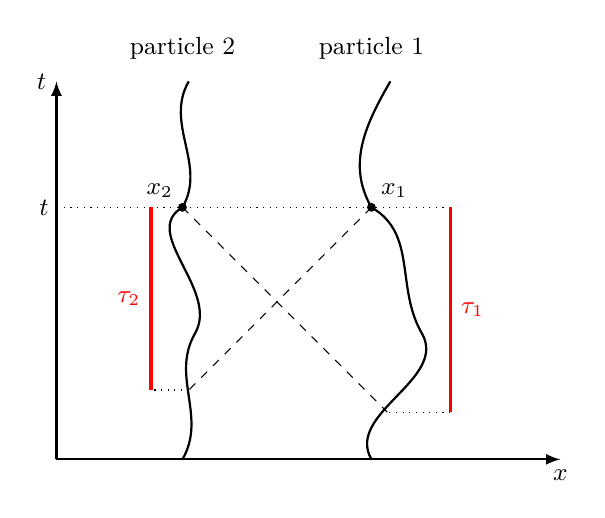
\begin{tikzpicture}[>=latex, every node/.style={font=\small}, scale=0.8]
  % Axes
  \draw[thick, ->](0,0) -- (0,6) node[left] {$t$};
  \draw[thick, ->] (0,0) -- (8,0) node[below] {$x$};

  % Particle 2 worldline (left)
  \coordinate (P2start) at (2,0);
  \coordinate (P2mid)   at (2.2,2);
  \coordinate (P2evt)   at (2,4);
  \coordinate (P2top)   at (2.1,6);
  \draw[thick] (P2start) to[out=60,in=240] (P2mid) 
                to[out=60,in=210] (P2evt) 
                to[out=60,in=240] (P2top);

  % Particle 1 worldline (right)
  \coordinate (P1start) at (5,0);
  \coordinate (P1mid)   at (5.8,2);
  \coordinate (P1evt)   at (5,4);
  \coordinate (P1top)   at (5.3,6);
  \draw[thick] (P1start) to[out=120,in=-60] (P1mid) 
                to[out=120,in=-30] (P1evt) 
                to[out=120,in=-120] (P1top);

  % Events x1 and x2
  \fill (P1evt) circle (2pt) node[above right] {$x_1$};
  \fill (P2evt) circle (2pt) node[above left]  {$x_2$};

  % Dotted equal-time slice
  \draw[dotted] (6.25, 4) -- (0,4);
  \node at (-0.2, 4) {\(t\)};

  \draw[dotted] (6.25, 0.75) -- (5.25,0.75);
  \draw[dotted] (2.1, 1.1) -- (1.5, 1.1);
  

  % Spacelike dashed path
  \draw[dashed] (P1evt) -- (2.1,1.1);
  \draw[dashed] (P2evt) -- (5.25,0.75);


  % Constant-time slices (red)
  \draw[red,very thick] (1.5,1.1) -- (1.5,4)
    node[left,midway] {$\tau_2$};
  \draw[red,very thick] (6.25, 0.75) -- (6.25, 4)
    node[right,midway] {$\tau_1$};

  % Labels for worldlines
  \node at (2,6.2) [above] {particle 2};
  \node at (5,6.2) [above] {particle 1};
\end{tikzpicture}
\end{figure}
    
    \begin{equation}
        F_{12} = F(x_2(t-\tau_2), \dot{x_2}(t-\tau_2), \dots, x_1(t), \dot{x_1}(t), \dots)
    \end{equation}
    and similarly
    \begin{equation}
        F_{21} = F'(x_1(t-\tau_1), \dot{x_1}(t-\tau_1), \dots, x_2(t), \dot{x_2}(t), \dots)
    \end{equation}
    In such an equation, the \(\tau_1\) and \(\tau_2\) themselves are dynamically determined, and depend on the entire past history of the two particles, and therefore in order to determine the dynamics of the particles, one needs to keep track of functions, which have infinite degrees of freedom. \\

    That said, even in classical dynamics, imposing STR postulates demands infinite number of degrees of freedom. 

    \subsection{Quantizing the STR Dynamics}
    In dealing with such systems, we encounter \textit{retarded differential equations}, or also called as \textit{functional differential equations}. And nobody knows how to quantize the system starting from the functional differential equations.\\

    Passage from CM to QM relies strongly on the idea that we are given an initial surface and we have a Hamiltonian/Lagrangian on it.\\
    In a Hamiltonian system we have a phase space and we see how stuff evolves in that space. In the above discussed case, we have to deal with an infinite number of degrees of freedom and these degrees of freedom are not in the form that is convenient to put in the Hamiltonian formalism.\\

    Fields solve this problem by rather than saying that particle 1 interacts with particle 2, we say particle 1 interacts with a field, and particle 2 too interacts with the field. The field and the particles influence each other only locally. In introducing this formalism we paid a price, we introduced infinite number of degrees of freedom in the form of fields, at the effect of removing the necessity of having to track all particle histories. The field can be thought of as keeping track of the history of the particles. In the language of fields, nothing depends on retarded times. \\

    With the introduction of fields, we now have everything in the language of phase space. We are given an initial surface, and data on it, and we can evolve everything into future. But rather than having only finite degrees of freedom we still need to keep track of infinite degrees of freedom of the fields, but they are now in a form convenient to quantize.\\

    \subsection{Another Reason Why We Need Infinite DOFs}
    Heisenberg's uncertainity principle — \(\Delta x \Delta p \ge1 \)\\
    If we have small \(\Delta x\), then \(\Delta p \) becomes large, such that \(\Delta E \ge m\). In this case we are now uncertain if we are dealing with the original particle, or if we have created a new particle. It is convenient therefore, to discuss the particles as excitations of fields, using which one can describe variable number of particles.\\

    ALSO fields explain why all electrons are identical.\\

    \subsection{Regular QM Breaks Causality}
    This is a very generic calculation that can be found in almost all lectures/texbooks. But still included here for completeness. \\

    The regular, single particle quantum mechanics that we all know of and are familiar with breaks causality. Causality requires that a particle can never move faster than the speed of light, i.e.\ a particle initially localised around the position \(\textbf{x}\) should not have any amplitude to move out of the future light cone. Now in the case of single particle QM, consider a particle localised about \(\textbf{x}\), described by state \(\ket{\textbf{x}}\).\\

    Suppose the particle follows the relativistic Hamiltonian, \(\hat H = \sqrt{\hat{\textbf{p}}^2 + m^2}\), the state of the particle after time \(t\) would be \(\exp(-i H t) \ket{\textbf{x}}\). Relativity requires that this state should have zero overlap with \(\ket{\textbf{x}'}\) where \((t, \textbf{x})\) and \((t, \textbf{x}')\) are spacelike separated.\\

    Let \(G(\textbf{x},\textbf{x}') = \braket{\textbf{x}' | \exp(-iHt) \textbf{x}}\). The explicit value of \(G\) can be calculated by inserting the identity in \(\ket{\textbf{p}}\) as follows.

    \begin{equation}
        G(\textbf{x}, \textbf{x}', t) = \int \frac{d^3\textbf{p}}{(2\pi)^3} \braket{\textbf{x}' | \exp(-i\sqrt{\hat{\textbf{p}}^2 + m^2} t) | \textbf{p}} \braket{\textbf{p}|\textbf{x}} = \int \frac{d^3\textbf{p}}{(2\pi)^3} \exp(-i\sqrt{\textbf{p}^2 + m^2} t)\braket{\textbf{x}'| \textbf{p}} \braket{\textbf{p}|\textbf{x}}
    \end{equation}
    \begin{equation}
        G(\textbf{x},\textbf{x}', t) = \int \frac{d^3\textbf{p}}{(2\pi)^3}  \exp(-i\sqrt{\textbf{p}^2 + m^2} t) \exp(-i \textbf{p}\cdot(\textbf{x}-\textbf{x}'))
    \end{equation}
    Write \(\textbf{x} - \textbf{x}' = \textbf{r}\), and align the \(z\) axis to be about \(\textbf{r}\). Then we can convert the above integral into polar coordinates as (where we use \(p = |\textbf{p}|\) and \(r = |\textbf{r}|\))
    \begin{align}
        G(\textbf{r}, t) &= \int \frac{p^2}{(2\pi)^2} \exp(-i\sqrt{p^2 + m^2} t) \exp(-i p r \cos\theta)~ dp d(\cos\theta)\\
        &= \int \frac{p^2}{(2\pi)^2} \exp(-i\sqrt{p^2 + m^2} t) \left( \frac{\exp(-ipr) - \exp(ipr)}{pr} \right)dp\\
        &= \frac{2}{(2\pi)^2}\frac{1}{r}\int \exp(-i\sqrt{p^2 + m^2} t)~ p ~\sin(pr)~dp
    \end{align}
    You can look up this integral in some Russian textbook and find out that this is equal to 
    \begin{equation}
        G \propto K_2 (m\sqrt{r^2 + t^2}) 
    \end{equation}
    This is some finite non-zero number (although it might be small for some values) for all \(r\) and \(t\). Since we require causality to be exactly held, and not approximately held, single particle quantum mechanics breaks causality.

    \newpage
    \section{Classical Field Theory}
    Everything we discussed previously does not logically conclude that the \textit{only} candidates are fields, but fields provide a convenient formalism, and end up solving the problems we were facing. \\

    In general, field is something associated with spacetime. That is, for every spacetime point, it spits out some mathematical entity. For the field, we would like to write a Lagrangian, as an integral of some Lagrangian density over all space. 
    \begin{equation}
        L = \int\ld ~d^3\textbf{x}
    \end{equation}
    We consider Lagrangian densities of the form 
    \begin{equation}
        \ld(\del_\mu \phi(x), \phi(x))
    \end{equation}
    (where we assume the notation \(x = (t, \textbf{x})\)). In principle, the Lagrangian density can be anything, but mostly we consider the most simple forms. We usually start with something that is quadratic in fields and their derivatives. Linear term is ignored since it can be absorbed into the quadratic term by considering a shift by constant factor of the fields leading to the a quadratic Lagrangian.\\
    Example — suppose
    \begin{equation}
        \ld = \frac{1}{2} (\del_\mu \phi)^2 - \frac{1}{2}m^2 \phi^2 - \alpha \phi
    \end{equation}
    consider the transformation \(\phi(x) \to \phi(x) + \displaystyle\frac{\alpha}{m^2}\), with \(\alpha\) being some spacetime independent constant. 
    \begin{equation}
        \ld' = \frac{1}{2} \left( \del_\mu \left(\phi' - \frac{\alpha}{m^2}\right)\right)^2 - \frac{1}{2} m^2 \left(\phi'^2 - 2\frac{\alpha}{m^2} \phi' + \left(\frac{\alpha}{m^2}\right)^2\right) - \alpha \phi = \frac{1}{2} (\del_\mu \phi')^2 - \frac{1}{2}m^2 \phi'^2
    \end{equation}
    (dynamics doesn't change when a constant term is added to the Lagrangian) which is a Lagrangian density with only quadratic terms. 

    \subsection{Dynamics in Classical Field Theory}
    \subsubsection{Lagrangin Dynamics}
    Action — \(S = \int \ld~d^4x\)
    \begin{center}
        \fbox{Nature is lazy}
    \end{center}
    Classical equations of motion — field configurations such that variation of \(S\) under \(\phi \to \phi + \delta\phi\) is zero. \\
    Under such change, 
    \begin{equation*}
        \delta S = \int \frac{\delta \ld}{\delta \del_\mu \phi}\delta(\del_\mu \phi) + \frac{\delta \ld}{\delta \phi}\delta(\phi) ~d^4x
    \end{equation*}
    \begin{equation}
        = \int -\delta\phi \del_\mu\frac{\delta \ld}{\delta \del_\mu \phi} + \delta\phi\frac{\delta \ld}{\delta \phi} + \del_\mu \left( \delta\phi \frac{\delta \ld}{\delta \del_\mu \phi} \right)~d^4x  
    \end{equation}
    Considering variations which vanish at infinity, the last term (which is only a boundary term) vanishes. The other two functions also should vanish for every possible values of \(\delta \phi\), therefore we get the equations of motions to be 
    \begin{equation}
        \del_\mu\frac{\delta \ld}{\delta \del_\mu \phi} - \frac{\delta \ld}{\delta \phi} = 0
    \end{equation}

    \subsubsection{Hamiltonian Dynamics}
    In order to make a passage to QFT, we need a Hamiltonian formulation. In going to Hamiltonian formulation, we trade the \textit{time derivative} with the \textit{conjugate momentum}.\\

    The basic degrees of freedom in classical mechanics were the spatial points \(\textbf{x}\). In the case of the field theory, the basic degrees of freedom are just the fields at a certain instant of time (which we conveniently call \(t=0\)) \(\psi(\textbf{x})\). The \(\del_i \phi(\textbf{x})\) are nothing but linear combinations of the \(\phi(\textbf{x})\), and in going to the Hamiltonian formulation, we treat the time derivative as a different degree of freedom.

    \begin{equation}
        \Pi(t=0, \textbf{x}) = \dot{\phi}(t=0, \textbf{x})
    \end{equation}

    The Hamiltonian is then 
    \begin{equation}
        H(t) = \int \Pi \dot{\phi} - \ld ~d^3\textbf{x} = \int \hd~d^3\textbf{x}
    \end{equation}
    and one can write equations similar to the Hamiltonian equations of motion for the field and its conjugate momenta.

    \subsection{Parameterizing the Phase Space}
    \label{sec:solution-freescalar}
    Given the phase space, the usual parameterization is using \(\Pi\) and \(\Phi\). But we can also parameterize the phase space using different variables — the set of solutions to the equations of motion. This is true because given a point in phase space, we can use it as initial conditions and obtain a solution to the equations of motion. Therefore, there is a one-to-one map between points in phase space and solutions to the equations of motion, and we can see the set of solutions to the equations of motion as parameterizing the phase space. That is, a point corresponds to a solution, and a solution provided a section corresponds to a point.\\
    In other words, the \textit{parameterization} of all solutions to the equations of motion is the same as parameterization of the whole phase space. \\

    For concreteness, let us start considering a specific theory — the scalar free field theory. 
    \begin{equation}
        \ld = \frac{1}{2}\left((\del_\mu \phi)^2 - m^2\phi^2\right)
    \end{equation}
    The equation of motion arising from this lagrangian is simply 
    \begin{equation}
        (\del_\mu \del^\mu + m^2)\phi(x) = (\del_t^2 - \nabla^2 + m^2)\phi(x) = 0
    \end{equation}
    We want to find all possible solutions to this equations of motion in order to parameterize the phase space. To find a parameterization for the solution of the equations of motion, the easiest way is to go to the fourier space. \\
    Writing \(\phi(t, \textbf{x}) = \int d^3\textbf{p} \phi(t, \textbf{p})\exp(i\textbf{p}\cdot\textbf{x})\), we get 
    \begin{equation}
        \int (\del_t^2 + \textbf{p}^2 + m^2)\phi(t, \textbf{p}) d^3\textbf{p} = 0
    \end{equation}
    We are keeping time as it is because in Hamiltonian formulation we require solutions at a given slice of time. \\
    The solutions to the above equation of motion is (with \(\w_\textbf{p} = \sqrt{\textbf{p}^2 + m^2}\))
    \begin{equation}
        \phi(t,\textbf{p}) = a(\textbf{p})\exp(-i \w_\mathbf{p} t) + b(\textbf{p}) \exp(i \w_\mathbf{p} t)
    \end{equation}
    Since we require \(\phi(t, \textbf{x})^* = \phi(t, \textbf{x})\), we need 
    \(\phi(t, \textbf{p})^* = \phi(t, -\textbf{p})\), meaning
    \begin{equation*}
        a^*(\textbf{p})\exp(i \w_\mathbf{p} t) + b^*(\textbf{p}) \exp(-i \w_\mathbf{p} t) = a(-\textbf{p})\exp(-i \w_\mathbf{p} t) + b(-\textbf{p}) \exp(i \w_\mathbf{p} t)
    \end{equation*}
    Comparing, we get \(b(\textbf{p}) = a^*(-\textbf{p})\), therefore, the solutions are 
    \begin{equation}
        \phi(t, \textbf{p}) = a(\textbf{p}) \exp(-i\w_\textbf{p} t) + a^*(-\textbf{p}) \exp(i\w_\textbf{p} t)
    \end{equation}
    and 
    \begin{equation}
        \phi(t, \textbf{x}) = \int a(\textbf{p}) \exp(-i\w_\textbf{p} t + i\textbf{p}\cdot \textbf{x}) + a^*(\textbf{p}) \exp(i\w_\textbf{p} t - i\textbf{p}\cdot \textbf{x}) ~ \frac{1}{\sqrt{2\w_\textbf{p}}} \frac{d^3 \textbf{p}}{(2\pi)^3} 
    \end{equation}
    where in second term, we did the change \(\textbf{p}\to -\textbf{p}\) since the integral is invarient under this change, and \(\displaystyle\frac{1}{\sqrt{2\w_\textbf{p}}}\) is simply a choice of normalisation.\\

    We can also write this as 
    \begin{equation}
        \phi(x) = \int a(p) \exp(-ip.x) + a^*(p) \exp(ip.x) ~\frac{1}{\sqrt{2\w_\textbf{p}}} \frac{d^3 \textbf{p}}{(2\pi)^3} 
    \end{equation}
    where now \(p\) and \(x\) are 4-vectors.\\

    The coordinates on the phase space are \(\phi(t=0, \textbf{x})\) and \(\Pi(t=0, \textbf{x})\), and in this case the parameterization is very clear that 
    \begin{equation}
        \phi(t=0, \textbf{x}) = \int a(\textbf{p}) \exp(i\textbf{p}\cdot \textbf{x}) + a^*(\textbf{p}) \exp(- i\textbf{p}\cdot \textbf{x}) ~ \frac{1}{\sqrt{2\w_\textbf{p}}} \frac{d^3 \textbf{p}}{(2\pi)^3}
    \end{equation}
    and 
    \begin{equation}
        \Pi(t=0, \textbf{x}) = \int -i \left(a(\textbf{p}) \exp(i\textbf{p}\cdot \textbf{x}) - a^*(\textbf{p}) \exp(- i\textbf{p}\cdot \textbf{x}) \right)~ \sqrt{\frac{\w_\textbf{p}}{2}} \frac{d^3 \textbf{p}}{(2\pi)^3}
    \end{equation}
    Rather than parameterizing the phase space using the field and conjugate momentum, we can parameterize using the \(a(\textbf{p})\) and \(a^*(\textbf{p})\). We can also invert these relations to write \(a\) and \(a^*\) in terms of field and momenta.
    \begin{equation}
        a(\textbf{p}) = \sqrt{\frac{\w_\textbf{p}}{2}}\int\phi(0, \textbf{x}) \e^{-i \textbf{p}. \textbf{x}}d^3\textbf{x} + \frac{i}{\sqrt{2\w_\textbf{p}}}\int \Pi(0, \textbf{x})\e^{-i \textbf{p}.\textbf{x}} d^3\textbf{x} 
    \end{equation}
    \begin{equation}
        a^*(\textbf{p}) = \sqrt{\frac{\w_\textbf{p}}{2}}\int\phi(0, \textbf{x}) \e^{i \textbf{p}. \textbf{x}}d^3\textbf{x} - \frac{i}{\sqrt{2\w_\textbf{p}}}\int \Pi(0, \textbf{x})\e^{i \textbf{p}.\textbf{x}} d^3\textbf{x} 
    \end{equation}\\

    \textcolor{red}{
        In order to understand this better, let us do the same analysis for the simpler classical mechanical system of a harmonic oscillator. The equation of motion is 
        \begin{equation*}
            ( \del_t^2 + \w^2 )x = 0
        \end{equation*} This is solved simply by 
        \begin{equation*}
            x(t) = \frac{1}{\sqrt{2\w}}\left(A\exp(-i\w t) + A^*\exp(i\w t)\right) ~~~\because~x\text{ is real}
        \end{equation*}
        where the prefactor is simply a choice of normalisation, and 
        \begin{equation*}
            p(t) = -i\sqrt{\frac{\w}{2}} (A\exp(-i\w t) - A^* \exp(i \w t))
        \end{equation*}
        The coordinates on the phase space are \(x(t=0)\) and \(p(t=0)\), which in this case are 
        \begin{equation*}
            x = \frac{1}{\sqrt{2\w}}(A + A^*)~~\&~~p = -i\sqrt{\frac{\w}{2}} (A - A^*)
        \end{equation*}
        For every \(x, p\), there is a solution \(A\) (where \(A\) is complex) that has \((x,p)\) as its initial conditions, and therefore the set of \(A\) can be thought of as parameterizing the entire phase space. This is exactly what is done in introducing the ladder operators for quantizing the harmonic oscillator. Instead of imposing the quantization condition on the usual coordinates \(x\) and \(p\), one uses the coordinates \(A\) and \(A^*\) and quantizes these degrees of freedom. \\
        Important! — There can be confusion in what one calls a solution to the equation of motion. One might be tempted to assume that, for example in this case, the set of ellipses in the phase space to be the set of solutions to the equations of motions. This is wrong, in the sense that the solutions for motion with initial state \(x_1, p_1\) and with initial state \(x_2, p_2\), even if both lie on the same ellipse, are different. Therefore, given an initial point in phase space, we determine a unique equation that governs this initial point's evolution and this equation is termed a solution. Therefore, corresponding to every point on the phase space, there is a unique solution, and therefore a bijection.  \\      
        }

        \textcolor{red}{
            We can further extend the above discussion by looking at the commutator relations of \(A\) and \(A^*\), which is given by 
            \begin{equation*}
                \{x,p\} = 1 \implies \{A^*, A\} = -i, ~\{A, A\}=0,\{A^*, A^*\} = 0 
            \end{equation*}
            We can also construct the Hamiltonian in terms of the variables \(A\) and \(A^*\), which is given as 
        \begin{equation*}
            H = \frac{1}{2}(p^2 + \w^2x^2) = \frac{1}{2}\w(A^*A+ AA^*) \tag{\(\star\)}
            \label{eq:ham_in_class}
        \end{equation*}
        This reduces to 
        \begin{equation*}
            H = \w A^* A
        \end{equation*}
        The commutators of Hamiltonian with the variables \(A^*\) and \(A\) are 
        \begin{equation*}
            \{H, A^*\} = \w A^*,~~~\{H, A\} = -\w A 
        \end{equation*}
        Notice that all of these are classical calculations, and invokes no quantum mechanics. 
        }
    
    \newpage
    \section{Quantizing the Fields}
    To quantize a theory, we take a set of \textit{coordinates} on phase space, and promote them to operators and impose the commutation relations.\\
    In case of multiple particles in the regular quantum mechanics, the commutation relation that we used to impose was 
    \begin{equation*}
        [x_i, p_j] = i\delta_{ij}
    \end{equation*}
    Similarly, the \(\phi(0, \textbf{x})\) and \(\Pi(0, \textbf{x})\) behave like multiple degrees of freedom, this time instead of labeled by a discrete index \(i\), they are labeled by a continous index \(x\). Therefore, we impose a similar commutation relation
    \begin{equation}
        [\phi(t, \textbf{x}), \Pi(t, \textbf{y})] = i\delta^3(\textbf{x} - \textbf{y})
    \end{equation} 
    \textcolor{red}{
    Notice that these are equal time commutation relations, i.e., this is imposed on one time slice. This is true even in the single particle quantum mechanics, where the canonical commutation relations hold only at equal times, i.e. 
    \begin{equation*}
        [x(t), p(t')] \ne i,~[x(t), x(t')] \ne 0,~[p(t), p(t')]\ne 0
    \end{equation*}
    As an example, consider the harmonic oscillator, 
    \begin{equation*}
        x(t) = \frac{1}{\sqrt{2\w}}(A\exp(-i\w t) + A^*\exp(i\w t))
    \end{equation*}
    \begin{equation*}
        p(t) = -i\frac{\sqrt{\w}}{2}(A\exp(-i\w t) - A^*\exp(i\w t))
    \end{equation*}
    The equal time commutation relation implies 
    \begin{equation*}
        [x(0), p(0)] = i[A, A^*] = i \implies [A, A^*] = 1\text{,~~ and } [A, A] = [A^*,A^*] = 0 
    \end{equation*}
    Using this, 
    \begin{equation*}
        [x(t), x(t')] = \frac{1}{2\w}\left(\e^{i\w(t'-t)}[A, A^*] + \e^{i\w(t-t')}[A^*, A]\right) = \frac{1}{2\w}\cos(\w(t'-t)) \ne 0
        \tag{\(\diamondsuit\)}
        \label{eq:time_comm}
    \end{equation*}
    }

    In terms of \(a(\textbf{p})\) and \(a^\dagger(\textbf{p})\) (where we are now calling \(a^* \equiv a^\dagger\) since we have promoted it to an operator), the commutation relations are 
    \begin{equation*}
        [a(\mathbf{p_1}), a^\dagger(\mathbf{p_2})] = \frac{-i}{2}\int[\phi(0, \mathbf{x_1}), \Pi(0, \mathbf{x_2})]\e^{-i\mathbf{p_1}\cdot \mathbf{x_1}}\e^{i\mathbf{p_2}\cdot \mathbf{x_2}} d^3\mathbf{x_1} d^3\mathbf{x_2} + \frac{i}{2}\int [\Pi(0, \mathbf{x_1}), \phi(0, \mathbf{x_2})]\e^{-i\mathbf{p_1}\cdot \mathbf{x_1}}\e^{i\mathbf{p_2}\cdot \mathbf{x_2}} d^3\mathbf{x_1} d^3\mathbf{x_2}
    \end{equation*}
    \begin{equation}
        = \int \delta^3(\mathbf{x_1} - \mathbf{x_2}) \e^{-i\mathbf{p_1}\cdot \mathbf{x_1}}\e^{i\mathbf{p_2}\cdot \mathbf{x_2}} d^3\mathbf{x_1} d^3\mathbf{x_2} = (2\pi)^2\delta^3(\mathbf{p_1} - \mathbf{p_2})
    \end{equation}
    It also holds that
    \begin{equation}
        [a(\textbf{p}), a(\textbf{q})] = [a^\dagger(\textbf{p}), a^\dagger(\textbf{q})] = 0
    \end{equation}
    \subsection{Hamiltonian in terms of the creation and annihilation operators}
    The expression for Hamiltonian of the theory is 
    \begin{equation}
        H = \frac{1}{2}\int \Pi(0,\textbf{x})^2 + (\nabla \phi(0, \textbf{x}))^2+ m^2\phi(0, \textbf{x})^2 ~d^3\textbf{x}
    \end{equation}
    Calculating this term wise (note that for brevity, we are now calling \(a(\textbf{p}) \equiv a_\textbf{p}\). See that \(a_\textbf{p}\) is not a number, but a function of \(\textbf{p}\)).
    \begin{equation*}
        \frac{1}{2}\int \Pi(0,\textbf{x})^2~d^3\textbf{x} =\frac{1}{2}\int d^3\textbf{x}\frac{d^3\textbf{p}d^3\textbf{q}}{(2\pi)^6}\frac{\sqrt{\w_\textbf{p}\w_\textbf{q}}}{2}\left(-a^\dagger_\textbf{p}a^\dagger_\textbf{q}\e^{i(\textbf{p}+\textbf{q})\cdot \textbf{x}}    
        +a^\dagger_\textbf{p}a_\textbf{q}\e^{i(\textbf{p}-\textbf{q})\cdot \textbf{x}} 
        + a_\textbf{p}a^\dagger_\textbf{q}\e^{-i(\textbf{p}-\textbf{q})\cdot \textbf{x}}   
        - a_\textbf{p}a_\textbf{q}\e^{-i(\textbf{p}+\textbf{q})\cdot \textbf{x}}  
           \right)  
    \end{equation*}
    The integral over \(\textbf{x}\) gives delta functions, and then we can perform an integral over \(\textbf{q}\) to remove the delta function, leading to the simplification
    \begin{equation}
        \frac{1}{2}\int \Pi(0,\textbf{x})^2~d^3\textbf{x} = \frac{1}{2}\int \frac{d^3\textbf{p}}{(2\pi)^3}\frac{\w_\textbf{p}}{2}(-a_\textbf{p}^\dagger a_{-\textbf{p}}^\dagger + a_\textbf{p}^\dagger a_\textbf{p} + a_\textbf{p}a_\textbf{p}^\dagger - a_\textbf{p}a_{-\textbf{p}})
    \end{equation}

    \begin{equation*}
        \frac{1}{2}\int (\nabla \phi(0, \textbf{x}))^2 d^3\textbf{x} = \frac{1}{2} \int d^3\textbf{x}\frac{d^3\textbf{p}d^3\textbf{q}}{(2\pi)^6}\frac{\textbf{p}\cdot \textbf{q}}{2\sqrt{\w_\textbf{p}\w_\textbf{q}}}\left(  
            - a^\dagger_\textbf{p}a^\dagger_\textbf{q}\e^{-i(\textbf{p} + \textbf{q})\cdot \textbf{x}} + a^\dagger_\textbf{p} a_\textbf{q} \e^{i(\textbf{p} - \textbf{q})\cdot \textbf{x}} + a_\textbf{p} a^\dagger_\textbf{q} \e^{-i(\textbf{p} - \textbf{q})\cdot \textbf{x}} - a_\textbf{p} a_\textbf{q} \e^{i(\textbf{p} + \textbf{q})\cdot \textbf{x}}
        \right)
    \end{equation*}
    which again simplifies to 
    \begin{equation}
        \frac{1}{2}\int (\nabla \phi(0, \textbf{x}))^2 d^3\textbf{x} = \frac{1}{2} \int \frac{d^3\textbf{p}}{(2\pi)^3}\frac{\textbf{p}^2}{2\w_\textbf{p}}(a_\textbf{p}^\dagger a_{-\textbf{p}}^\dagger + a_\textbf{p}^\dagger a_\textbf{p} + a_\textbf{p}a_\textbf{p}^\dagger + a_\textbf{p}a_{-\textbf{p}})
    \end{equation}
    and similarly
    \begin{equation}
        \frac{1}{2}\int m^2 \phi(0, \textbf{x})^2 d^3\textbf{x} = \frac{1}{2} \int \frac{d^3\textbf{p}}{(2\pi)^3}\frac{m^2}{2\w_\textbf{p}}(a_\textbf{p}^\dagger a_{-\textbf{p}}^\dagger + a_\textbf{p}^\dagger a_\textbf{p} + a_\textbf{p}a_\textbf{p}^\dagger + a_\textbf{p}a_{-\textbf{p}})
    \end{equation}
    Adding the above three equations, using the fact that \(\w^2_\textbf{p} = \textbf{p}^2 + m^2\), we get 
    \begin{equation}
        H = \frac{1}{2}\int  \frac{d^3\textbf{p}}{(2\pi)^3} \w_\textbf{p} (a_\textbf{p}^\dagger a_\textbf{p} + a_\textbf{p}a_\textbf{p}^\dagger ) 
        \label{eq:hamiltonian}
    \end{equation}

    \subsection{Momentum of Fields}
    Claim — Momentum (not the conjugate momentum, but rather the physical momentum) has the form 
    \begin{equation}
        \textbf{P} = -\int d^3\textbf{x}\Pi(0, \textbf{x}) \mathbf{\nabla} \phi(0, \textbf{x}) 
    \end{equation}
    Why?\\
    We can see that  
    \begin{equation*}
        [\textbf{P}, \phi(0, \textbf{x})] = -i\mathbf{\nabla}\phi(0, \textbf{x})
    \end{equation*}
    Given this commutation relation, we can write, therefore, that 
    \begin{equation}
        \phi(0, \textbf{x} + \mathbf{\epsilon}) = \e^{-i\textbf{P}\cdot\mathbf{\epsilon}}\phi(0, \textbf{x})\e^{i\textbf{P}\cdot\mathbf{\epsilon}} = \phi(0, \textbf{x}) - i[\mathbf{\epsilon}\cdot\textbf{P}, \phi(0, \textbf{x})] = \phi(0, \textbf{x}) + \mathbf{\epsilon}\cdot \mathbf{\nabla}\phi(0, \textbf{x})
    \end{equation}
    Therefore the operator \(\textbf{P}\) generates translations.\\

    In terms of \(a\) and \(a^\dagger\) (the calculation is simple, except that at the end we drop some terms owing to \textit{normal ordering} which will be discussed later) 
    \begin{equation}
        \textbf{P} = \int \frac{d^3\textbf{p}}{(2\pi)^3} \textbf{p}a^\dagger_\textbf{p} a_\textbf{p}
    \end{equation}

    \subsection{Why \(a^\dagger\) and \(a\) are Creation and Annihilation Operators}
    Given the form of Hamiltonian in terms of \(a\) and \(a^\dagger\), we immediately see that 
    \begin{equation}
        [H, a^\dagger_\textbf{p}] = \w_\textbf{p}a^\dagger_\textbf{p},~~~[H, a_\textbf{p}] = -\w_\textbf{p}a_\textbf{p}
    \end{equation}
    which means that for a stationary state \(\ket{E}\) with energy \textbf{E} the operators \(a^\dagger_\textbf{p}\) and \(a_\textbf{p}\) map it to another state with energy \(E+\w_\textbf{p}\) and \(E-\w_\textbf{p}\)
    \begin{equation}
        H(a^\dagger_\textbf{p}\ket{E}) = (E + \omega_p)(a^\dagger_\textbf{p}\ket{E}),~~~ H(a_\textbf{p}\ket{E}) = (E - \omega_p)(a_\textbf{p}\ket{E})
    \end{equation}
    This behavior is exactly the same as that of a harmonic oscillator, and therefore the free Klein-Gordon theory is exactly a decoupled set of infinite harmonic oscillators. 

    \subsection{Constructing the Hilbert Space}
    \subsubsection{Vacuum}
    In order to construct the Hilbert space, we need to start with a vacuum, which is the state with the lowest energy. \\
    Since vacuum has the lowest energy, operating on it with any \(a_\textbf{p}\) should annihilate the state. Therefore, the state vacuum is defined as the state 
    \begin{equation*}
        a_\textbf{p}\ket{0} = 0 ~~\forall \textbf{p}
    \end{equation*}
    The energy of vacuum is 
    \begin{equation*}
        H\ket{0} = \frac{1}{2}\int \frac{d^3\textbf{p}}{(2\pi)^3}\w_\textbf{p} a_\textbf{p} a^\dagger_\textbf{p}\ket{0} =  \frac{1}{2}\int  d^3\textbf{p} \delta^3(0) \w_\textbf{p} \ket{0}
    \end{equation*}
    where we picked the \(\delta(0)\) by commuting the \(a\) and \(a^\dagger\). The result states that the vacuum has infinite energy, which is expected since there are infinite number of harmonic oscillators and each of the oscillator contribute to a finite zero-point energy.\\

    We don't have to worry about this so much because we are able to physically measure only the energy differences, in which case we can set, by-hand, the energy of vacuum to be 0. Another reason why we need not worry is because we are not even sure if the expression for the Hamiltonian is right. This is because when going from classical to quantum theory, there is an inherent ambiuity in operator ordering, and it is upto us to choose what ordering we use. 
    As an example, consider a term \(xp\) in classical physics. How do you write the corresponding operator? There is an ambiguity in whether it will be \(\hat x \hat p\) or \(\hat p \hat x\) or even \(\displaystyle\frac{\hat x \hat p + \hat p \hat x}{2}\) or any other combination. For an example in the case of harmonic oscillator see equation (\ref{eq:ham_in_class}), where the classical variables in the Hamiltonian commute, but there will be an ambiguity in the ordering when promoting the variables to operators. \\

    One convenient choice is to place all the annihilation operator to the right and all the creation operators to the left, and it is called normal ordering, and is denoted as \(\normord{\hat{O}}\). \\

    The normal ordered Hamiltonian is 
    \begin{equation}
        \normord{H} = \int \frac{d^3\textbf{p}}{(2\pi)^3} \w_\textbf{p} a^\dagger_\textbf{p} a_\textbf{p}
    \end{equation}
    and with this choice of \(H\), we get 
    \begin{equation*}
        \normord{H}\ket{0} = 0
    \end{equation*}
    
    \subsubsection{First Excited States} 
    There are an infinite number of first excited states given by 
    \begin{equation*}
        a^\dagger_\textbf{p}\ket{0}
    \end{equation*}
    The energy of these states is \(\w_\textbf{p}\) (since \(\ket{0}\) has energy 0), and momentum
    \begin{equation*}
        \textbf{P}(a^\dagger_\textbf{p}\ket{0}) = \int \frac{d^3\textbf{q}}{(2\pi)^3} \textbf{q}a^\dagger_\textbf{q}a_\textbf{q}a^\dagger_\textbf{p}\ket{0} = \int \frac{d^3\textbf{q}}{(2\pi)^3} \textbf{q}a^\dagger_\textbf{q}(a^\dagger_\textbf{p}a_\textbf{q} + \delta^3(\textbf{p} - \textbf{q}))\ket{0} = \textbf{p}a^\dagger_\textbf{p}\ket{0}
    \end{equation*}
    The energy and momentum indeed satisfy the dispersion relation \(\w_\textbf{p}^2 = \textbf{p}^2 + m^2\), and therefore these are to be interpreted as single particle states. \\

    The normalisation of these states is given as 
    \begin{equation}
        \braket{\textbf{p}|\textbf{q}} = \braket{0|a_\textbf{p}a^\dagger_\textbf{q}|0} = \braket{0|a^\dagger_\textbf{q}a_\textbf{p} + (2\pi)^3\delta^3(\textbf{p}-\textbf{q})|0} = (2\pi)^3\delta^3(\textbf{p}-\textbf{q})
    \end{equation}
    Delta function normalisation does not make any sense physically. Therefore in order to produce a normalisable state, we need to smear the operator, i.e. create a wavepacket
    \begin{equation*}
        \ket{f} = \int f(\textbf{p}) \ket{\textbf{p}} \frac{d^3\textbf{p}}{(2\pi)^3}
    \end{equation*}
    and for this state the normalisation is given by 
    \begin{equation*}
        \braket{f'|f} = \int f'(\textbf{q}) \ket{\textbf{q}} f'(\textbf{p}) \ket{\textbf{p}} \frac{d^3\textbf{p}d^3\textbf{q}}{(2\pi)^6} = \int f'(\textbf{p})f(\textbf{p}) \frac{d^3\textbf{p}}{(2\pi)^3}
    \end{equation*}
    These are not the only states in the Hilbert space of the system, there are other states too.

    \subsubsection{Higher Excited States}
    We can act with multiple creation operators to create higher excited states which can also be interpreted as \(n\)-particle states. As an example, let us check the state \(a^\dagger_\textbf{q}a^\dagger_\textbf{p}\ket{0}\). 
    \begin{equation*}
        H(a^\dagger_\textbf{q}a^\dagger_\textbf{p}\ket{0}) = \w_\textbf{q} + \w_\textbf{p}
    \end{equation*}
    and 
    \begin{align*}
        P(a^\dagger_\textbf{q}a^\dagger_\textbf{p}\ket{0}) &= \int \frac{d^3\textbf{r}}{(2\pi)^3}\textbf{r}a^\dagger_\textbf{r}a_\textbf{r}a^\dagger_\textbf{q}a^\dagger_\textbf{p}\ket{0} \\
        &=\int \frac{d^3\textbf{r}}{(2\pi)^3}\textbf{r}a^\dagger_\textbf{r}( a^\dagger_\textbf{q}a_\textbf{r} +\delta^3(\textbf{q} - \textbf{r}) )a^\dagger_\textbf{p}\ket{0} \\
        &=\int \frac{d^3\textbf{r}}{(2\pi)^3}\textbf{r}a^\dagger_\textbf{r}\delta^3(\textbf{q} - \textbf{r})a^\dagger_\textbf{p}\ket{0}  + \int \frac{d^3\textbf{r}}{(2\pi)^3}\textbf{r}a^\dagger_\textbf{r}a^\dagger_\textbf{q}(a^\dagger_\textbf{p} a_\textbf{r} + \delta^3(\textbf{p} - \textbf{r}))\ket{0} \\
        &= (\textbf{p} + \textbf{q})(a^\dagger_\textbf{q}a^\dagger_\textbf{p}\ket{0} )
    \end{align*}
    Therefore this state has total energy equal to the sum of the energies of one particle states with momentum \(\textbf{p}\) and \(\textbf{q}\), and total momentum equal to the vector sum of the two momenta. Therefore this state can be interpreted as a two particle state with the two particles having the same mass \(m\) and different momenta \(\textbf{p}\) and \(\textbf{q}\).\\

    The two particle states obey bosonic statistics. We can see this by noticing that \(a^\dagger_\textbf{p}\) commutes with \(a^\dagger_\textbf{q}\), and therefore the states \(\braket{\textbf{q}, \textbf{p}}\equiv a^\dagger_\textbf{q}a^\dagger_\textbf{p}\ket{0}\) and \(\braket{\textbf{p}, \textbf{q}} \equiv a^\dagger_\textbf{p}a^\dagger_\textbf{q}\ket{0}\) are the same states. Therefore, these particles automatically satisfy Bose-Einstein statistics, and there is no need to introduce these statistics by hand.\\

    The normalisation of the two particle states can be found as 
    \begin{align*}
        \braket{\mathbf{p_2}, \mathbf{q_2} | \mathbf{p_1}, \mathbf{q_1}} &= \braket{0|\a{p_2}\a{q_2} \adag{p_1}\adag{q_1}|0}\\
        &= \braket{0|\a{p_2} \adag{p_1} \a{q_2} \adag{q_1}|0} + (2\pi)^3\delta^3(\mathbf{q_2} - \mathbf{p_1})\braket{0|\a{p_2}\adag{q_1}|0} \\
        &= \braket{0|\a{p_2} \adag{p_1}|0} (2\pi)^3\delta^3(\mathbf{q_2} - \mathbf{q_1})+ (2\pi)^6\delta^3(\mathbf{q_2} - \mathbf{p_1})\delta^3(\mathbf{p_2} - \mathbf{q_1}) \\
        &= (2\pi)^6\delta^3(\mathbf{q_2} - \mathbf{q_1})\delta^3(\mathbf{p_2} - \mathbf{p_1})+ (2\pi)^6\delta^3(\mathbf{q_2} - \mathbf{p_1})\delta^3(\mathbf{p_2} - \mathbf{q_1}) 
    \end{align*}

    For proper normalisation, we can look at states of the kind 
    \begin{equation*}
        \ket{f} = \int f(\textbf{p}, \textbf{q}) \ket{\textbf{p}, \textbf{q}} \frac{d^3\textbf{p}d^3\textbf{q}}{(2\pi)^6} 
    \end{equation*}
    The smearing function should be symmetric in \(\textbf{p}\) and \(\textbf{q}\), because if there were an antisymmetric part, the bosonic statistics of the state will lead to a zero under the integral.\\
    
    Similarly we can construct \(n\) particle states, with \(n\) going all the way to \(\infty\), by repeated application of creation operators of the respective momenta.\\

    \subsubsection{The Fock Space}    
    With this, we have done all the possible things we could have done on the vacuum, and have generated all the possible states of the theory. Therefore the Hilbert space of the theory is the direct sum 
    \begin{equation}
        \mathbb{H} = \oplus_{n=0}^{\infty}\mathbb{H}_n
    \end{equation}
    where \(\mathbb{H}_n\) is the Hilbert space with \(n\) particles.This is called a Fock Space. In this we are summing over spaces which are orthogonal to each other. \\
    
    \textcolor{red}{
        Check that the one particle states are orthogonal to two particle states.
        \begin{equation*}
            \braket{\textbf{p}, \textbf{q} | \textbf{r}} = \braket{0| \a{p}\a{q}\adag{r}|0} = \braket{0|\a{p}\adag{r}\a{p}|0} + (2\pi)^3\delta^3(\textbf{q} - \textbf{r})\braket{0|\a{p}|0} = 0
        \end{equation*}
        Similarly one can show that the individual spaces are orthogonal to each other.\\
    }

    We can therefore write projectors onto different spaces. 
    \begin{equation*}
        P_0 = \ket{0}\bra{0}
    \end{equation*}
    \begin{equation*}
        P_1 = \int  \frac{d^3\textbf{p}}{(2\pi)^3} \ket{\textbf{p}}\bra{\textbf{p}}
    \end{equation*}
    Why is this a projector? \\
    \begin{equation*}
        P_1^2 = \int  \frac{d^3\textbf{p}d^3\textbf{q}}{(2\pi)^6} \ket{\textbf{p}}\bra{\textbf{p}} \ket{\textbf{q}}\bra{\textbf{q}} = \int  \frac{d^3\textbf{p}}{(2\pi)^3} \ket{\textbf{p}}\bra{\textbf{p}} = P_1
    \end{equation*}
    The projector on 2-particle states is naively
    \begin{equation*}
        P_2 = \int  \frac{d^3\textbf{p}d^3\textbf{q}}{(2\pi)^6} \ket{\textbf{p}, \textbf{q}}\bra{\textbf{p}, \textbf{q}} 
    \end{equation*}
    This is not the complete picture since, 
    \begin{equation*}
        P_2 \ket{\mathbf{k_1}, \mathbf{k_2}} = 2\ket{\mathbf{k_1}, \mathbf{k_2}}
    \end{equation*}
    (use the normalisation derived above, and the fact that the particles are bosons.)\\
    Therefore, we need a prefactor 
    \begin{equation*}
        P_2 = \frac{1}{2!}\int  \frac{d^3\textbf{p}d^3\textbf{q}}{(2\pi)^6} \ket{\textbf{p}, \textbf{q}}\bra{\textbf{p}, \textbf{q}} 
    \end{equation*}
    and therefore, the projector to \(n\)-particle state would be 
    \begin{equation*}
        P_n = \frac{1}{n!}\int  \frac{d^3\mathbf{p_1}\cdots d^3\mathbf{p_n}}{(2\pi)^{3n}} \ket{\mathbf{p_1},\cdots, \mathbf{p_n}}\bra{\mathbf{p_1},\cdots, \mathbf{p_n}} 
    \end{equation*}

    The identity therefore would be 
    \begin{equation*}
        \mathbb{I} = \sum_{i=0}^\infty P_i
    \end{equation*}
    
    \newpage
    \section{Detour — Schrodinger Representation}
    So far we discussed \textit{one} representation of the Hilbert Space. Here we will discuss another representation called the Schrodinger representation. (Hattfeld — QFT of particles and strings, and Polchinski — String theory).

    \subsection{The Schrodinger Equation}

    Initially we told that field theory is not different from QM, but so far we have not discussed any wavefunctions or Schrodinger equation governing the evolution of the wavefunction. It is indeed possible to do so, just that it is not a convenient picture to speak about the fields in terms of. Here we discuss the picture a bit.\\

    We started our quantization procedure through the commutation relations
    \begin{equation}
        [\phi(0, \textbf{x}), \Pi(0, \textbf{x}')] = i\delta^3(\textbf{x} - \textbf{x}')
    \end{equation}
    There is also a natural way to also represent states, which is to think of wavefunctions on the different degrees of freedom, i.e. in this case it will become a wavefunctional 
    \begin{equation}
        \psi[\phi(0,\textbf{x})]
    \end{equation}
    In normal QM, if you give a value of \(\textbf{x}\) at an instant of time, it spits out a c-number. In the case of QFT, when you give a field configuration in space at an instant of time, the wavefunctional gives a c-number. \\

    An example of such a wavefunction is 
    \begin{equation}
        \psi[\phi] = \e^{-\int \phi(0, \textbf{x})^2d^3\textbf{x}}
    \end{equation}
    The constraint on the possible functionals is that it should be normalisable.\\

    How does the momentum acts on the wavefunction?\\
    Claim — The momentum operator is given by the following operator on the wavefunction 
    \begin{equation}
        \Pi(0, \textbf{x}) = -i\frac{\delta}{\delta\phi(0, \textbf{x})}
    \end{equation}
    To check that this is indeed the form of momentum operator, check
    \begin{align*}
        [\phi(0, \textbf{x}), \Pi(0, \textbf{y})]\psi &= -i\left( \phi(0, \textbf{x}) \frac{\delta}{\delta \phi(0, \textbf{y})} \psi - \frac{\delta}{\delta \phi(0, \textbf{y})}(\phi(0, \textbf{x}) \psi)  \right)\\
        &=i \delta^3(\textbf{x} - \textbf{y})\psi       
    \end{align*}
    as required.\\

    \textcolor{red}{
        We can also check that the momentum operator acts as translation operator on the wavefunctional when we perform a shift on the field configuration. An infinitesimal shift in the field configuration is of the form 
        \begin{equation}
            \phi(0, \textbf{x}) \to \phi(0, \textbf{x}) + \epsilon \varphi(0, \textbf{x})
        \end{equation}
        Under such a transformation, the wavefunctional transforms as 
        \begin{equation}
            \psi[\phi(0, \textbf{x}) + \epsilon \varphi(0, \textbf{x})] \approx \psi[\phi(0, \textbf{x})] + \epsilon \varphi(0, \textbf{x})\frac{\delta }{\delta  \phi(0, \textbf{x})}\psi[\phi(0, \textbf{x})] = \e^{i\epsilon\varphi(0, \textbf{x}) \left( -i\frac{\delta}{\delta \phi(0, \textbf{x})} \right)}\psi[\phi(0, \textbf{x})]
        \end{equation}
        If we require momentum operator to generate these translations, then the momentum operator must be indeed of the form 
        \begin{equation}
            \Pi(0, \textbf{x}) = -i\frac{\delta}{\delta \phi(0, \textbf{x})}
        \end{equation}
        Therefore, the theory has three momentums which one can talk about — the conjugate momentum to \(\textbf{x}\) - \(\textbf{p}\) which generates translations in space, the physical momentum operator \(\textbf{P}\) which generates translations of fields in space, i.e. \(\phi(0, \textbf{x}) \to \phi(0, \textbf{x} + \textbf{a})\), and has as eigenvalues the total momentum of the excitations, and the momentum conjugate to the fields, \(\Pi\) which generates the translations of wavefunctional under shifts in field configurations, i.e. \(\psi[\phi] \to \psi[\phi + \varphi]\).\\
        In a similar language as QM, we can also write wavefunctions in other spaces such as momentum space in configuration space, by making a fourier transformation of \(\psi[\phi]\) with respect to \(\Pi\) and converting to \(\psi[\Pi]\) given as 
        \begin{equation}
            \psi[\Pi] = \int \D \phi ~\psi[\phi] \e^{-i\int \phi \Pi d^3\textbf{x}}
        \end{equation}
        but at this point, such a fourier transform has no use to it in our disccussions.\\
    }

    We can also write a Schrodinger equation given as 

    \begin{equation}
        i\frac{\del}{\del t}\psi[\phi] = \int -\frac{\delta^2}{\delta \phi^2} \psi[\phi] + (\nabla \phi)^2\psi[\phi]+ m^2\phi^2\psi[\phi]  ~~d^3\textbf{x}
    \end{equation}
    which governs the time evolution of the wavefunctional.

    \subsection{The Vacuum in Schrodinger Formulation}
    The defining property of vacuum is that the annihilation operators annihilate the vacuum. 
    It is convenient to introduce the fourier transform 
    \begin{equation}
        \phi(0, \textbf{p}) = \int \phi(0, \textbf{x}) \e^{-i\textbf{p}\cdot \textbf{x}}d^3\textbf{x}
    \end{equation}
    \begin{equation}
        \Pi(0, \textbf{p}) = \int \Pi(0, \textbf{x}) \e^{-i\textbf{p}\cdot \textbf{x}}d^3\textbf{x}
    \end{equation}
    In terms of these, the commutation relation is 
    \begin{equation}
        [\phi(0, \textbf{p}), \Pi(0, \textbf{q})] = \int [\phi(0, \textbf{x}), \Pi(0, \textbf{y})]\e^{-i\textbf{p}\cdot\textbf{x}}\e^{-i\textbf{q}\cdot \textbf{y}} d^3\textbf{x}d^3\textbf{y} = i(2\pi)^3\delta^3(\textbf{p}+\textbf{q})
    \end{equation}
    The action of \(\Pi(0, \textbf{p})\) on \(\psi\) is given by 
    \begin{equation}
        \Pi(0, \textbf{p})\psi[\phi(0, \textbf{q})] = -i(2\pi)^3\frac{\delta}{\delta \phi(0, -\textbf{p})}\psi[\phi(0, \textbf{q})]
    \end{equation}

    \textcolor{red}{
        To check that this is true, see that
        \begin{equation}
            [\psi(0, \textbf{p}), \Pi(0, \textbf{q})]\psi = -i(2\pi)^3 \left( \phi(0, \textbf{p}) \frac{\delta}{\delta \phi(0,-\textbf{q})}\psi - \frac{\delta}{\delta(\phi(0, -\textbf{q}))} (\phi(0, \textbf{p})\psi)\right) = i(2\pi)^3\delta^3(\textbf{p}-~(-\textbf{q}))
        \end{equation}
        which is indeed the required relation.\\
    }

    We had 
    \begin{equation}
        a_\textbf{p} = \sqrt{\frac{\w_\textbf{p}}{2}}\int\phi(0, \textbf{x}) \e^{-i \textbf{p}. \textbf{x}}d^3\textbf{x} + \frac{i}{\sqrt{2\w_\textbf{p}}}\int \Pi(0, \textbf{x})\e^{-i \textbf{p}.\textbf{x}} d^3\textbf{x} 
    \end{equation}
    which now becomes 
    \begin{equation}
        a_\textbf{p} = \sqrt{\frac{\w_\textbf{p}}{2}}\phi(0, \textbf{p}) + \frac{i}{\sqrt{2\w_\textbf{p}}}\Pi(0,\textbf{p})
    \end{equation}
    The vacuum is the state that is annihilated by \(a_\textbf{p}\) which gives the equation
    \begin{equation}
        \sqrt{\frac{\w_\textbf{p}}{2}}\phi(0, \textbf{p}) \psi_0[\phi] -i(2\pi)^3 \frac{i}{\sqrt{2\w_\textbf{p}}}\frac{\delta}{\delta \phi(0, -\textbf{p})}\psi_0[\phi] = 0
    \end{equation}
    This is solved by 
    \begin{equation}
        \psi_0 = \displaystyle\e^{-\frac{1}{2}\int \w_\textbf{p} \phi(0, \textbf{p})\phi(0, -\textbf{p})\frac{d^3\textbf{p}}{(2\pi)^3}}
    \end{equation}
    Since \(\phi(0, \textbf{x})\) is real field, we need that \(\psi(0, -\textbf{p}) = \psi(0, \textbf{p})^*\). Therefore the solution is an exponential of squares, which means it is a Gaussian, as was in the case of harmonic oscillator. Notice that this ground state is not normalised. In such a formalism, the expectation values are to be written as 
    \begin{equation}
        \braket{A} = \displaystyle \frac{\int \D \phi ~ \psi[\phi]^2 A[\phi] }{\int \D \phi ~ \psi[\phi]^2}
    \end{equation}
    and therefore the normalisation doesn't matter as it gets cancelled when taking the ratios.\\

    Similarly we can also write the wavefunctionals for higher excited states by acting upon with \(a^\dagger_\textbf{p}\)s.

    \newpage
    \section{Causality}
    Before discussing causality, we need a notion of what are the observables in a QFT. 

    \subsection{Observables in QFT}
    In quantum mechanics all Hermitian operators are observables. When transitioning to QFT, we need to modify our notion of the observables. In QFT, observables are tied to spacetime points.\\

    Observables are of the form \(O(x)\) (where \(x\) is now a spacetime point). We can define observables in a region \(R\) as 
    \begin{equation}
        \int_R O(x) f(x) d^4x
    \end{equation}
    We can also construct operator like 
    \begin{equation}
        \int_{\bar{R}} O(x) g(x) d^4x
    \end{equation}
    where \(\bar{R}\) is the region complement to \(R\), and this operator is NOT an observable in \(R\).\\

    \subsection{Does QFT Preserve Causality}

    Suppose \(R\) and \(R'\) are spacelike separated regions. Then causality requires that observations in \(R\) should be independent of observations in \(R'\). What this means is that observations in \(R\) should not affect, and should not be affected by observations in \(R'\). What this implies is that 
    \begin{equation}
        [O(R) , \tilde O(R')] = 0
    \end{equation}
    This doesn't mean that observation in \(R\) should be uncorrelated with observations in \(R'\). They can be correlated as in entanglement, but they should not be able to affect each other. Notice that we have always used this notion in our regular quantum mechanics, where we say that when measuring one observable does not affect the value of another should imply that they have a simultaneous set of eigenvalues and therefore the operators must commute. Here we are running a similar argument. \\

    All observables in our theory are polynomials in \(\phi\). Therefore causality requires that 
    \begin{equation}
        [\phi(x), \phi(y)] = 0\text{, if }(x-y)^2 <0
    \end{equation}
    On a single time slice, this is true and is a canonical commutation relation, since every \(\textbf{y}\) is disconnected from \(\textbf{x}\). But causality requires this to be true also for any \(x\) and \(y\) at different times, but spacelike separated. (The commutator relation above being satisfied at \(t=0\) doesn't guarentee that it will be satisfied at some other \(t\) as can be seen in the example (\ref{eq:time_comm}))\\

    Is this criteria satisfied in our theory?\\
    We can explicitly calculate this commutator as follows 
    \begin{equation*}
        \phi(x) = \int \a{p}\e^{-ip\cdot x} + \adag{p}\e^{ip\cdot x} \frac{d^3\textbf{p}}{(2\pi)^3\sqrt{2\w_\textbf{p}}}
    \end{equation*}
    \begin{equation*}
        \implies [\phi(x), \phi(y)] = \int [\a{p}, \adag{q}]\e^{-ip\cdot x + iq\cdot y} + [\adag{q}, \a{p}]\e^{ip\cdot x - iq\cdot y}\frac{d^3\textbf{p}d^3\textbf{q}}{(2\pi)^62\sqrt{\w_\textbf{p}\w_\textbf{q}}}
    \end{equation*}
    \begin{equation*}
        = \int \e^{-ip\cdot(x-y)} - \e^{ip\cdot(x-y)}\frac{d^3\textbf{p}}{(2\pi)^32\w_\textbf{p}}~~
    \end{equation*}
    The LHS is Lorentz invarient, but on RHS, we see that the integral is over \(d^3\textbf{p}\). The RHS should still be Lorentz invarient. To see how we can write the integral in a covariant form, consider the following integral first
    \begin{equation}
        \int d^4p \delta^4(p^2 - m^2) \theta(p^0)
        \label{eq:lor_inv_meas}
    \end{equation}
    Now this integral is manifestly Lorentz invarient, because it has an integral over \(d^4p\), a \(\delta\) function in \(p^2 - m^2\) and a \(\theta\) function in \(p^0\). The \(\theta\) function is also Lorentz invarent since \(\delta\) function fixes that \(p^2 = m^2 >0\), making \(p\) a timelike vector, and there is no Lorentz transformation that can change the sign of the time component of a timelike vector. The \(theta\) function is also needed since we initially started with a specific sign of \(\w\), that is \(\w_p >0\). If we choose the other sign, then the result will not be that of the integral we are trying to evaluate.\\
    We can do this integral as 
    \begin{align*}
        &\int d^3\textbf{p}dp^0 \delta(p_0^2 - \textbf{p}^2 - m^2)\delta(p^0)\\
        =& \int d^\textbf{p}dp^0 \frac{\delta(p_0 - \w_p)}{2p_0}\\
        =& \int \frac{d^3\textbf{p}}{2\w_p}
    \end{align*}
    Therefore, the commutator can be written as a Lorentz invarient integral 
    \begin{equation}
        [\phi(x), \phi(y)] = \int \e^{-ip\cdot(x-y)} - \e^{ip\cdot(x-y)}\frac{1}{(2\pi)^3}d^4p \delta^4(p^2 - m^2) \theta(p^0)
    \end{equation}
    When \(x\) and \(y\) are spacelike separated, there is a Lorentz transformation that takes \(x-y\) to \(-(x-y)\). An explicit example would be to first boost to a frame where \(x\) and \(y\) are simultaenous, making \(x-y = (0, \mathbf{\Delta})\), and then a rotation of the \(3-\)vector by 180 degree taking it to \((0.-\mathbf{\Delta}) = -(x-y)\). Notice that this is not possible when \(x\) and \(y\) are timelike separated, since there is no frame of reference where they are simultaneous. Therefore, when \(x\) and \(y\) are timelike separated, the second integral can be Lorentz transformed to match the first integral, and therefore the difference between them, which gives the commutator, is zero.\\

    We also need to check that the commutator is not identically zero when the separation is timelike. To check this, we need to explicitly evaluate the integral by converting it into polar coordinates.  \\
    Consider the integral 
    \begin{align*}
        f(q) &= \int e^{-ip\cdot q} \frac{d^3\textbf{p}}{(2\pi)^3{2\w_\textbf{p}}} = \e^{-i\w_p q^0} \int \e^{i\textbf{p}\cdot \textbf{q}} \frac{d^3\textbf{p}}{(2\pi)^3{2\w_\textbf{p}}}\\
        &= \e^{-i\w_p q^0} \int \e^{ipq\cos\theta} p^2 dp d\cos\theta\frac{1}{(2\pi)^2{2\w_\textbf{p}}} \text{where now }p~\&~q\text{ stand for } |\textbf{p}|~\&~|\textbf{q}|\\
        &= \e^{-i\w_p q^0}\int_0^\infty \frac{1}{iq}\left(  \e^{ipq} - \e^{-ipq}  \right) pdp \frac{1}{(2\pi)^2{2\w_\textbf{p}}}
    \end{align*}
    Since the integral is invarient under the transformation \(p\to-p\), we can do the transformation for the second piece, and then flip the integration limits, to obtain 
    \begin{align*}
        f(q) &= \e^{-i\w_p q^0}\int_0^\infty \frac{1}{iq} \e^{ipq} pdp \frac{1}{(2\pi)^2{2\w_\textbf{p}}} + \e^{-i\w_p q^0}\int_{-\infty}^0 \frac{1}{iq} \e^{ipq} pdp \frac{1}{(2\pi)^2{2\w_\textbf{p}}}\\
        &=\e^{-i\w_p q^0}\int_{-\infty}^\infty \frac{1}{iq} \e^{ipq} pdp \frac{1}{(2\pi)^2{2\w_\textbf{p}}}\\
        &= \frac{-i}{4\pi q} \frac{\del}{\del q} \int_{-\infty}^{\infty} \e^{-i\w_p q^0+ipq} \frac{dp}{2\pi\w_p} 
    \end{align*}
    Now, we can make the substitutions 
    \begin{align*}
        \w_p = m\cosh\phi ~~&\&~~ p = m\sinh \phi \implies \frac{dp}{\w_p} = d\phi\\
        q^0 = \alpha \cosh\phi_0 ~~&\&~~ q = \alpha\sinh \phi_0 
    \end{align*}
    This substitution also preserves the relations between \(\w_p\) \& \(p\) and \(q^0\) \& \(q\). Also we are taking \(q^0\) with \(\cosh\) because we are looking at the case where \(q^0\) is large compared to \(q\).\\

    With this, we can write the integral as 
    \begin{equation*}
        f(q) = \frac{-i}{4\pi q} \frac{\del}{\del q} \int_{-\infty}^\infty \e^{-im\alpha \cosh(\phi -\phi_0)} \frac{d\phi}{2\pi} 
    \end{equation*}
    This integral has the value 
    \begin{equation*}
        f(q) = \frac{1}{4\pi} \frac{\del}{\del q} \left(-\frac{i}{2} \mathrm{sgn}(q^0) J_0(m\alpha) - N_0(m\alpha)\right)
    \end{equation*}
    (there seems to be some errors in the calculation. If you are able to rectify please send your calculations by email!)\\
    The commutator in the case \(x-y\) is timelike is therefore 
    \begin{equation*}
        [\phi(x), \phi(y)] = \frac{i}{4\pi} \mathrm{sgn}(x^0 - y^0) \frac{m}{\alpha} J_1(m\alpha)
    \end{equation*}
    We get this as, differentiation of \(J_0\) gives \(J_1\) and when taking the Hermitian conjugate of the above integral and subtracting it to get the commutator, the term proportional to \(N_1\) cancels. It should not be surprising that the answer is proportional to \(i\) since the commutator is an antihermitian quantity and therefore should be purely imaginary. \\

    The commutator is finite in timelike separations and exactly zero for spacelike separations. \\
    Therefore, causality is preserved in QFT.
    
    \subsection{Localized Excitations in QFT}
    \textcolor{red}{Before discussing localised excitations, let us first discuss what the action of \(\phi(x)\) on the vacuum is. We called \(\adag{p}\ket{0}\)s as the one particle states of our system. The \(\phi(x)\) is a linear combination of \(\adag{p}\)s, with different \(p\)s given different weights. Therefore, \(\phi(x)\ket{0}\) is a superposition of infinite number of one particle states with different momenta, and therefore is itself a one particle state. To create higher particle states, one needs to operate by more \(\phi(x)\)s \\}

    Now let us discuss how can one define localised excitations in some region \(R\)?\\
    Suppose we have a region \(R\), and an operator \(O\) in \(\bar{R}\) which is spacelike to \(R\)
    \begin{figure}[h]
        \centering 
        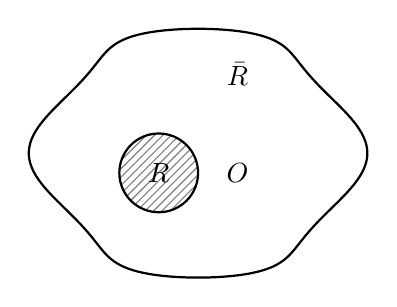
\begin{tikzpicture}
            \draw[thick]
                plot [domain=0:360, samples=200, smooth, variable=\t]
                    (
                        {0.5 + 2*cos(\t) + 0.15*cos(5*\t)},
                        {0.25 + 1.5*sin(\t) + 0.08*sin(1*\t)}
                    )
                    -- cycle;
            \fill[pattern=north east lines, pattern color=black!50] (0,0) circle (0.5);
            \draw[thick] (0,0) circle (0.5);
            \node at (0,0) {\(R\)};
            \node at (1,1.25) {\(\bar R\)};
            \node at (1, 0) {\(O\)};
        \end{tikzpicture}
    \end{figure}

    For an excitation \(\ket{\psi(R)}\) to be local in \(R\), we require that 
    \begin{equation*}
        \braket{\psi(R)|O(\bar{R}) | \psi(R)} = \braket{0|O(\bar{R})|0} ~~\forall~O \text{ in region spacelike to }R
    \end{equation*} 
    That is, the expectation values of operators in regions spacelike separated from \(R\) should be the same as their vacuum expectation values.  \\

    How can we create such a state?\\
    Our first guess would be 
    \begin{equation*}
        \ket{\psi(R)} = \int_R d^4x f(x) \phi(x) \ket{0} 
    \end{equation*}
    We can check if this is indeed a localised expectation, 
    \begin{equation*}
        \braket{\psi(R)|O(\bar{R})|\psi(R)} = \int f(x) f(y) \braket{0|\phi(x) O \phi(y) | 0}
    \end{equation*}
    since \(\phi\) in \(R\) and \(O\) in \(\bar{R}\) must commute, the above should be equal to 
    \begin{equation*}
        \braket{\psi(R)|O(\bar{R})|\psi(R)} = \int f(x) f(y) \braket{0|O\phi(x)  \phi(y) | 0}
    \end{equation*}
    which is not equal to the vacuum expectation value of \(O\). See that even \(\phi(z)\) does not produce a local excitation \textbf{at \(z\)}, since \(\phi(z)\) is obtained by simply setting \(f(x) = \delta(x-z), ~f(y) = \delta(z-y)\) in the above integral.  \\

    What do we need to create a localized excitation?\\
    In order for \(\ket{\psi(R)} = U(R)\ket{0}\) to be a localised excitation, we need 
    \begin{equation*}
        \braket{\psi(R)|O(\bar{R})|\psi(R)} = \braket{0|U^\dagger(R)O(\bar{R})U(R)|0} = \braket{0|O(\bar{R})U^\dagger(R)U(R)|0} = \braket{0|O(\bar{R})|0}
    \end{equation*}
    What this implies is that the operator \(U\) should satisfy \(U^\dagger U = I\), i.e.\ it should be unitary. Therefore 
    \begin{equation*}
        U(R) = \e^{i\int_R f(x)\phi(x) dx}\ket{0}
    \end{equation*}
    is a localised excitation in \(R\). There is no unique localised excitation, there can be many unitary operators in \(R\) that can produce localised excitations. One can also see that since \(\phi\) are Hermitian, the only way to create unitary operators is by exponentiating the \(\phi\)s with a factor of \(i\). If you produce an excitation in a region of space \(\textbf{R}\), it propagates outwards at the speed of light, such that all the region which is timelike to \(\textbf{R}\) is affected, while regions spacelike to \(\textbf{R}\) are not at all affected. \\
    
    Now these localised excitations can never be single particle states. Since the exponential can be written as 
    \begin{equation*}
        \e^{i\int_R f(x)\phi(x) dx}\ket{0} = \left(1 + i\int_R f(x)\phi(x) dx + \frac{1}{2}i\iint_R f(x)f(y)\phi(x)\phi(y) dxdy + \cdots \right)\ket{0}
    \end{equation*}
    the localised excitation is always a superposition of states of all possible particle numbers. 

    \newpage
    \section{Interlude — Symmetries}

    What we mean when we say that the action has symmetry is that when we make a change in the fields \(\phi_i(x) \to \phi_i(x) + \lambda D\phi_i(x)\), (where \(D\phi_i\) is just a notation and can denote any function, but is usually a function of original \(\phi_i\)s and \(\lambda\) is a parameter to keep track of order of terms), the action remains invariant. \\
    For this to be true, the Lagrangian density should transform as 
    \begin{equation*}
        \ld \to \ld + \del_\mu K^\mu
    \end{equation*}
    Now this invariance should hold for all the field configurations, and not just some special ones, i.e.\ the configurations which satisfy the equations of motion. For the configurations which satisfy the equations of motion, the requirement is identically satisfied, since we define the equations of motion as those configurations for which the small variations of fields do not change the action.\\ 

    \subsection{Noether's Theorem}
    When \(\ld\) has a symmetry, there is a conserved current of the form
    \begin{equation*}
        \del_\mu j^\mu = 0
    \end{equation*} 
    \textit{only for the solutions of the equations of motion}.\\

    Proof —\\
    Under the above transformation,
    \begin{align*}
        &\delta \ld = \left( \frac{\delta \ld}{\delta \phi_i} D\phi_i  + \frac{\delta \ld}{\delta \del_\mu \phi_i} \del_\mu D\phi_i \right) = \del_\mu K^\mu \\
        \implies & \left( \frac{\delta \ld}{\delta \phi_i} D\phi_i  -\del_\mu \frac{\delta \ld}{\delta \del_\mu \phi_i} D\phi_i + \del_\mu \left( \frac{\delta \ld}{\delta \del_\mu \phi_i} D\phi_i \right)  \right) = \del_\mu K^\mu 
    \end{align*}
    When we are on-shell (i.e. when \(\phi\) satisfies the equation of motion), the first two term sum to 0, and we are left with 
    \begin{equation*}
        \del_\mu \left( \frac{\delta \ld}{\delta \del_\mu \phi_i} D\phi_i \right) = \del_\mu K^\mu
    \end{equation*}
    which implies that  
    \begin{equation*}
        \del_\mu j^\mu(x) =0, ~\text{ where  } j^\mu = \frac{\delta \ld}{\delta \del_\mu \phi_i} D\phi_i  - K^\mu 
    \end{equation*}

    Noether's current is not something new, it is just re-expressing the equations of motion. Noether's current has inherent ambiguity in definition, because we can always add a divergence free \(4-\)vector to it, i.e.\ we can add terms of the form \(\epsilon^{\mu\nu} \del_\nu \phi\) where \(\epsilon\) is antisymmetric tensor, since \(\del_\mu \epsilon^{\mu\nu} \del_\nu \phi = 0\). But nevertheless this is a powerful statement and allows us to derive conclusions without having to do tedious calculations.\\

    When we have a conserved current, we have a conserved charge.
    \begin{equation*}
        \del_0 \int j^0 d^3\textbf{x} + \int d^3\textbf{x} \del_i j^i = 0 \implies \del_t \int j^0 d^3\textbf{x} = 0
    \end{equation*}
    since the second term is a total divergence. What this tells is that the quantity 
    \begin{equation*}
        Q = \int j^0 d^3\textbf{x}
    \end{equation*} 
    is conserved. All conservation of laws that we have known so far arise in this very fashion, and are consequences of the Noether's theorem.\\

    There is another derivation of the Noether's theorem, which is at the level of action. Suppose we have a symmetry under 
    \begin{equation*}
        \phi \to \phi + \lambda D\phi
    \end{equation*}
    which does not change \(S\).\\
    Now imagine a spacetime dependent variation, 
    \begin{equation*}
        \phi \to \phi + \lambda(x) D\phi
    \end{equation*}
    The action is not invarient under this transformation. The Lagrangian, upto first order in \(\lambda\) changes as 
    \begin{equation*}
        \ld \to \ld + \lambda(x) \del_\mu(K^\mu) + \del_\mu(\lambda(x)) P^\mu
    \end{equation*}
    since these are the only terms that are Lorentz invariant and first order in \(\lambda\).\\
    The action transforms as 
    \begin{align*}
        S \to &S + \int d^4x~ \lambda(x) \del_\mu(K^\mu) + \del_\mu(\lambda(x)) P^\mu\\
        = & S + \int d^4x ~ \lambda(x) \del_\mu (K^\mu - P^\mu)
    \end{align*}
    On solutions to equations of motions, the action should be invariant under these transformations too. Therefore 
    \begin{equation*}
        \del_\mu (K^\mu - P^\mu) = 0
    \end{equation*}
    Now what is \(P^\mu\)? \\
    Under the given transformation, the Lagrangian changes as 
    \begin{equation*}
        \ld \to \ld + \left( \frac{\delta \ld}{\delta \phi}\lambda(X) D\phi +  \frac{\delta \ld}{\delta \del_\mu \phi} \del_\mu(\lambda(x) D\phi) \right)
    \end{equation*}
    from which we can see that \(P^\mu\) is simply the part that multiplies to \(\del_\mu \lambda(x)\), which is 
    \begin{equation*}
        P^\mu = \frac{\delta \ld}{\delta \del_\mu \phi} D\phi
    \end{equation*}

    % We can also ask how the conserved charge transform under Lorentz transformation.\\

    % The conserved current is a \(4-\)vector, and therefore under Lorentz transformation transforms as
    % \begin{equation*}
    %     J^\mu(x) \to J'^{\mu}(x') = \Lambda\indices{^\mu_\nu}J^\nu (\Lambda^{-1} X)
    % \end{equation*}
    % The conserved charge is given by 
    % \begin{equation*}
    %     Q(t) = \int d^3\textbf{x} J^0(t, \textbf{x})
    % \end{equation*}
    % Now since this is conserved, we can choose one specific time to evaluate this, and for convenience we choose \(t=0\).\\
    % \begin{equation*}
    %     Q = \int d^3\textbf{x} J^0(0, \textbf{x})
    % \end{equation*}
    % We can also write this as the \(4-\)integral
    % \begin{equation*}
    %     Q = \int d^4x \delta(\eta\cdot x) \eta \cdot J(x)
    % \end{equation*}
    % where \(\eta = (1,0,0,0)\). This \(4-\)integral can be written as 
    % \begin{equation*}
    %     Q = \int d^4x \del_\mu \theta(\eta\cdot x)  J^\mu(x)
    % \end{equation*}
    % by noticing that the space-derivative of theta function is simply zero, and the time derivative gives the delta function multiplied by \(\eta_\mu\)
    

    \subsection{Applications}
    Let us look at some applications of the Noether's theorem
    \subsubsection{Spacetime translations}
    Consider \(x^\mu \to x^\mu + a^\mu\).\\
    When \(\ld\) doesn't explicitly depend on position, this is a symmetry. In the language of fields, this transformation is 
    \begin{equation*}
        \phi \to \phi + \lambda \del_\mu \phi^\mu 
    \end{equation*}
    where \(\lambda\) is just to keep track of orders.\\

    Since \(\ld\) is a Lorentz scalar, 
    \begin{equation*}
        \ld \to \ld + \lambda a^\mu \del_\mu \ld \implies K^\mu =  a^\mu \ld
    \end{equation*}

    Therefore, the conserved current is 
    \begin{equation*}
        j^\mu = \frac{\delta \ld}{\delta \del_\mu \phi}a^\nu  \del_\nu \phi  - a^\nu \delta_\nu^\mu \ld
    \end{equation*}
    Now this current is conserved for all possible \(a^\mu\) which means that 
    \begin{equation*}
        T_\nu^\mu = \frac{\delta \ld}{\delta \del_\mu \phi} \del_\nu \phi  -  \delta_\nu^\mu \ld \implies T^{\mu\nu} = \frac{\delta \ld}{\delta \del_\mu \phi} \del^\nu \phi  -  \eta^{\mu\nu} \ld
    \end{equation*}
    must be conserved. This is called stress-energy tensor and this is conserved. Let us check what this is for few cases 
    \begin{equation*}
        T^{00} = \frac{\delta \ld}{\delta \dot{\phi}}  \dot{\phi} - \ld = \mathcal{H}
    \end{equation*}
    which is the Hamiltonian density. Integrating this over all space gives the Hamiltonian which is the energy, and this shows that energy is conserved.
    \begin{equation*}
        T^{0i} = \frac{\delta \ld}{\delta \dot{\phi}} \del^i \phi
    \end{equation*}
    the corresponding conserved charge is 
    \begin{equation*}
        P^i =  \int d^3\textbf{x} \frac{\delta \ld}{\delta \dot{\phi}} \del^i \phi
    \end{equation*}
    which is nothing but the spatial momentum in \(i\)th direction as we had defined previously. The stress tensor therefore gives \(4\) conserved charges (we need to keep \(\mu = 0\) and integrate, and there are \(4\) choice of \(\nu\)) which are energy and the three components of momentum.\\ 

    The formula for stress-tensor is not manifestly symmetric in \(\mu\) and \(\nu\), but we can use the ambiguity that we discussed to subtract the antisymmetric part and make it symmetric. But in most cases of physical interest, stress-tensor is explicitly symmetric.

    \subsubsection{Lorentz transformation}
    Lorentz transformation 
    \begin{equation*}
        \tilde{x}^\mu = \Lambda\indices{^\mu_\nu} x^\nu
    \end{equation*}
    The requirement is that the transformation preserves vector inner products 
    \begin{equation*}
        \tilde{x}^\mu\tilde{y}^\nu \eta_{\mu\nu} = x^\mu y^\nu \eta_{\mu\nu} \implies \Lambda\indices{^\rho_\mu} \Lambda\indices{^\sigma_\nu} \eta_{\rho\sigma} =\eta_{\mu\nu} 
    \end{equation*}

    An infinitesimal transformation of \(x\) would be 
    \begin{equation*}
        x^\mu \to x^\mu + \lambda \epsilon\indices{^\mu_\nu} x^\nu
    \end{equation*}
    For this to be a Lorentz transformation 
    \begin{align*}
        &(x^\mu + \lambda \epsilon\indices{^\mu_\nu} x^\nu)(y_\mu + \lambda \epsilon\indices{_\mu_\nu} y^\nu) = x^\mu y_\mu \\
        \implies & x^\mu y_\mu + \lambda \epsilon\indices{^\mu_\nu} x^\nu y_\mu + \lambda\epsilon_{\mu\nu}x^\mu y^\nu + O(\lambda^2) = x^\mu y_\mu\\
        \implies & \epsilon_{\mu\nu}x^\nu y^\mu + \epsilon_{\mu\nu} x^\mu y^\nu = 0
    \end{align*}
    Now since in the first term, \(\mu\) and \(\nu\) are dummy indices, we can interchange them to get 
    \begin{equation*}
        \left(\epsilon_{\nu\mu}+ \epsilon_{\mu\nu}\right) x^\mu y^\nu = 0\implies  \epsilon_{\nu\mu}= - \epsilon_{\mu\nu}
    \end{equation*}
    Which implies that the \(\epsilon_{\mu\nu}\) is an antisymmetric tensor. (Notice that this would not work if we compare tensors with one upper and one upper index). There are 6 components to the antisymmetric tensor, and therefore 6 conserved currents — three for boosts and three for rotations. As an example consider \(\epsilon_{01} = 1,~\epsilon_{10} = -1\) rest all 0. Under this 
    \begin{equation*}
        \delta x^0 = \lambda x^1,~~\delta x^1 = \lambda x^0
    \end{equation*}
    which are infinitesimal boosts. If \(\epsilon_{12} = 1,~\epsilon_{21} = -1\), then 
    \begin{equation*}
        \delta x^1 = -\lambda x^2,~~\delta x^2 = \lambda x^1
    \end{equation*}
    This is an infinitesimal rotation. \\

    Under Lorentz transformation, the fields transform as 
    \begin{equation*}
        \delta x^\mu = \lambda \epsilon\indices{^\mu_\nu} x^\nu \implies \delta \phi =\lambda \del_\mu \phi \epsilon\indices{^\mu_\nu} x^\nu
    \end{equation*}

    Under this kind of transformation, the lagrangian density also transforms as 
    \begin{equation*}
        \delta \ld = \lambda (\del_\mu \ld) \epsilon\indices{^\mu_\nu} x^\nu 
    \end{equation*}
    Now since \(\del_\mu (\epsilon\indices{^\mu_\nu} x^\nu) = \delta\indices{^\nu_\mu}\epsilon\indices{^\mu_\nu} = \eta^{\mu\nu}\epsilon_{\mu\nu} = 0\) (\(\because\) \(eta\) is symmetric and \(\epsilon\) is antisymmetric) \textcolor{red}{(another way to look at this is that \(\delta\indices{^\nu_\mu}\epsilon\indices{^\mu_\nu} = \mathrm{Tr}\epsilon = 0\))} we can add this term to make the change in lagrangian density a total derivative 
    \begin{equation*}
        \delta ld = \lambda \del_\mu (\ld \epsilon\indices{^\mu_\nu} x^\nu)
    \end{equation*}
    To proceed, let us consider an explicit example of a theory, the lagrangian density we have already considered. For this theory, 
    \begin{equation*}
        \frac{\delta \ld}{\delta \del_\mu \phi} = \del^\mu \phi
    \end{equation*}
    and therefore, 
    \begin{equation*}
        j^\mu = \del^\mu \phi \del_\rho \phi \epsilon\indices{^\rho_\nu}x^\nu - \ld \epsilon\indices{^\mu_\nu} x^\nu
    \end{equation*}
    Since this should be conserved for all \(\epsilon\), we need to pull it out of the equation as 
    \begin{equation*}
        j^\mu = (\del^\mu \phi \del^\rho \phi x^\nu - \ld \eta\indices{^\rho^\mu} x^\nu)\epsilon\indices{_\rho_\nu}
    \end{equation*}
    The conserved current is therefore the antisymmetric part of 
    \begin{equation*}
        \del^\mu \phi \del^\rho \phi x^\nu - \ld \eta\indices{^\rho^\mu} x^\nu
    \end{equation*}
    since the derivative of the symmetric part is identically zero, owing to the presence of \(\epsilon\). Therefore the conserved current is 
    \begin{equation*}
        M^{\mu\nu\rho} = (\del^\mu \phi \del^\rho \phi x^\nu - \ld \eta\indices{^\rho^\mu} x^\nu) - (\rho\leftrightarrow \nu)
    \end{equation*}
    There are 6 possible choices of \(\rho\) and \(\nu\) for the antisymmetric part, and therefore 6 conserved currents. \\

    The above quantity is exactly equal to 
    \begin{equation*}
        M^{\mu\nu\rho} = x^\nu T^{\mu\rho} - x^\rho T^{\mu\nu}
    \end{equation*}
    where \(T\) is the stress tensor. The six conserved charges are 
    \begin{equation*}
        Q^{\nu\rho} = \int  x^\nu T^{0\rho} - x^\rho T^{0\nu} d^3\textbf{x}
    \end{equation*}

    The different cases —\\
    \begin{equation*}
        Q^{ij} = \int  x^i T^{0j} - x^j T^{0i} d^3\textbf{x}
    \end{equation*}
    This is angular momentum associated with the plane of rotation \(ij\).
    \begin{equation*}
        Q^{0i} = \int  x^0 T^{0i} - x^i T^{00} d^3\textbf{x}
    \end{equation*}
    Let us write it in a slightly different way. \(\int T^{01} d^3\textbf{x} = P^i\), meaning 
    \begin{equation*}
        Q^{0i} = tP^i - \int x^i T^{00} d^\textbf{x}
    \end{equation*}
    Differentiating with respect to time (and using momentum is conserved),
    \begin{equation*}
        P^i - \frac{d}{dt} \int x^i T^{tt} d^3\textbf{x} = 0 \implies P^i - \left(\int  T^{tt}d^3\textbf{x} \right)\times \frac{d}{dt} \frac{\int x^i T^{tt} d^3\textbf{x}}{\int  T^{tt} d^3\textbf{x}}
    \end{equation*}
    Since \(T^{tt}\) is simply the mass density, the integral in the brackets is simply the total mass, and the object getting differentiated is the position of the center of mass. That is 
    \begin{equation*}
        P^i = M\frac{d}{dt} x^i_{COM}
    \end{equation*}
    which is just the classical defninition of momentum. 

    \subsubsection{Internal Symmetries}
    So far we discussed transformations in \(\phi\) due to changes to spacetime. Now we will discuss something different. Consider a theory with two fields, 
    \begin{equation*}
        \ld = \frac{1}{2} (\del_\mu \phi_1)^2 + \frac{1}{2} (\del_\mu \phi_1)^2 - \frac{m^2}{2} \phi_1^2-\frac{m^2}{2} \phi_2^2
    \end{equation*} 
    This theory has a continous symmetry under rotations of \(\phi_1\) into \(\phi_2\), i.e. 
    \begin{equation*}
        \phi_1 \to \cos\theta \phi_1 - \sin\theta \phi_2,~~ \phi_2\to \cos\theta \phi_2 + \sin\theta \phi_1
    \end{equation*}
    This transformation leaves the lagrangian density unchanged. \\
    infinitesimally, the above transformation looks like 
    \begin{equation*}
        \delta \phi_1 = - \phi_2,~~\delta \phi_2 = \phi_1
    \end{equation*}
    The associated current is 
    \begin{equation*}
        j^\mu =  \phi_1 \del^\mu \phi_2 - \phi_2 \del^\mu \phi_1
    \end{equation*}
    The associated charge is 
    \begin{equation*}
        Q = \int \phi_1 \del^0 \phi_2 - \phi_2 \del^0 \phi_1 d^3\textbf{x}
    \end{equation*}
    Charges like electric charge etc.\ are of this form. \\

    These fields are real fields. However we can combine these two into one complex object as
    \begin{equation*}
        \chi = (\phi_1 + i\phi_2)\frac{1}{\sqrt{2}},~~\chi^* = (\phi_1 - i\phi_2)\frac{1}{\sqrt{2}}
    \end{equation*}
    With this, 
    \begin{equation*}
        \frac{1}{2}(\phi_1^2 + \phi_2^2) = |\chi|^2
    \end{equation*}
    and 
    \begin{equation*}
        \frac{1}{2} ((\del_\mu \phi_1)^2 + (\del_\mu \phi_2)^2) = |\del_\mu \chi|^2
    \end{equation*}
    Therefore, the Lagrangian density becomes
    \begin{equation*}
        \ld = |\del_\mu \chi|^2 - m^2 |\chi|^2
    \end{equation*}
    In this language, the symmetry is
    \begin{equation*}
        \chi \to \e^{i\alpha} \chi,~~\chi^* \to \e^{-i\alpha}\chi^*
    \end{equation*}
    The corresponding current is 
    \begin{equation*}
        j^\mu = i((\del_\mu \chi^*) \chi - (\del_\mu\chi)\chi^*)
    \end{equation*}
    Since \(phi_1\) and \(\phi_2\) transformed into each other, they are not the fields corresponding to particles of positive and negative charges.\ \(\chi\) and \(\chi^*\) are the fields that correspond to particles of positive and negative charges. This is an example of \(U(1)\) internal symmetry. We can have theories with more elaborate symmetries like \(SU(N), Sp(N)\) etc.

    \newpage 
    \section{Interactions}

    \textcolor{red}{Free field theory — theory whose Lagrangian density has only terms that are quadratic in fields. These are exactly solvable, as we did previously. Interacting theory — introducing any other in the Lagrangian will lead to interactions between the different fields or with itself.}\\

    So far, we discussed free field theories, and we want to extend our discussions interacting theories. Before that, let us discuss what kind of questions can we ask in the presence of interactions. 

    \subsection{The \(S-\)matrix}

    The most general kind of question would be 
    \begin{figure}[h]
        \centering
        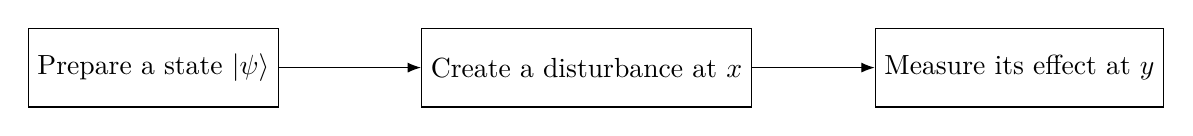
\begin{tikzpicture}[>=Latex,node distance=5.5cm]
            \node[draw, rectangle, minimum width=3cm, minimum height=1cm] (A) {Prepare a state \(\ket{\psi}\)};
            \node[draw, rectangle, right of=A, minimum width=3cm, minimum height=1cm] (B) {Create a disturbance at \(x\)};
            \node[draw, rectangle, right of=B, minimum width=3cm, minimum height=1cm] (C) {Measure its effect at \(y\)};

            % Draw the arrows
            \draw[->] (A) -- (B);
            \draw[->] (B) -- (C);

        \end{tikzpicture}
    \end{figure}
    
    Such questions are answered by computing the correlators of the form — \(\braket{0|\phi(x_1)\cdots\phi(x_n)|0 }\).\\

    However, it turns out that in QFT, although we can ask these questions, a lot of focus is on slightly \textit{simpler} questions.\\
    The simpler question is 
    \begin{figure}[h]
        \centering
        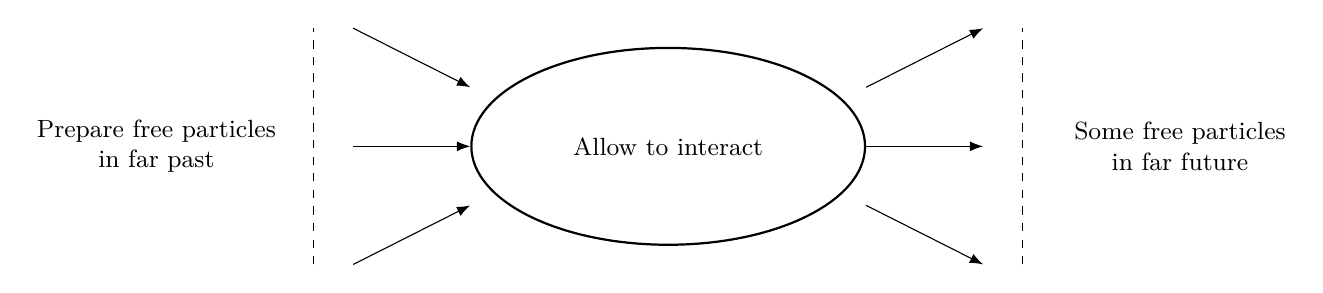
\begin{tikzpicture}[>=Latex, every node/.style={font=\small, align=center}]

            % Left and right text
            \node (in) at (-6.5,0) {Prepare free particles\\in far past};
            \node (out) at ( 6.5,0) {Some free particles \\in far future};

            \draw[dashed] (-4.5, -1.5) -- (-4.5, 1.5);
            \draw[dashed] (4.5, -1.5) -- (4.5, 1.5);

            \node[ellipse, draw, thick,
                minimum width=5cm, minimum height=2.5cm] (proc) 
            at (0,0) {Allow to interact};

            % Converging arrows (left → centre)
            %   start at (-6, +2),(-6,0),(-6,-2)
            %   end at proc.west + (0,+1),(0,0),(0,-1)
            \foreach \sy/\ey in {1.5/0.75, 0/0, -1.5/-0.75} {
                \draw[->] (-4,\sy) -- ($(proc.west)+(0,\ey)$);
            }

            % Diverging arrows (centre → right)
            %   start at proc.east + (0,+1),(0,0),(0,-1)
            %   end at (6,+2),(6,0),(6,-2)
            \foreach \ey/\sy in {0.75/1.5, 0/0, -0.75/-1.5} {
                \draw[->] ($(proc.east)+(0,\ey)$) -- (4,\sy);
            }

        \end{tikzpicture}
    \end{figure}

    That is, we create free particles in far past, let them evolve and interect, and ask what are the free particles and their properties in far future. This kind of question is answered by something called the \(S\) matrix. One might think that this is less general than the other question, but in fact it turns out that it has all the information we want to have about the theory. \\

    Why we talk about \(S\) matrix?
    \begin{enumerate}
        \item Experiments — most physics we learn from experiments is from this kind of experiments. 
        \item Theoretical reasons — two theoretical reasons \begin{itemize}
            \item \(S\) matrix is an unambigously decided observable. That is if we ask the question like what is the correlator 
            \begin{equation*}
                \braket{\psi | \phi(x_1) \cdots \phi(x_n)| \psi}
            \end{equation*}
            this is very ambigous. This is because in interacting theory, there is no unambigous \textit{definition} of field. One can always redefine the fields at the cost of adding interaction terms, without altering the physical content of the theory. When the fields are free and don't interact, there is `a' free field, and field redefinitions do not obey the equations of motions whereas the original field obeys. But in case of interacting theories, no fields obey the equation of motion, and therefore it is not clear how to choose what is the \textit{unique} field that we want to talk about.\\
            There is a class of field theories called conformal field theories, where there are other principles that allows one to uniquely identify field variables even in the case of interactions, and there we can talk about the first type of questions. But in general \(S\) matrix is unambigously defined since all we talk about is free theories in far past and future.
            \item In Quantum Gravity, maybe only the \(S\) matrix makes sense. The reason for that is that the first type of questions involve some local questions about what happens in some local regions of spacetime, and when the metric itself is fluctuating and spacetime itself is fluctuating, such questions are not well defined. But when we ask the second type of questions, in far past and future, where such fluctuations are not present, it is perfectly well defined. 
        \end{itemize}
    \end{enumerate}

    Therefore there are good reasons to consider the \(S\) matrix. Now we develop the machinery needed to calculate these \(S\) matrices. 

    \subsection{The Interaction Hamiltonian}
    For an interacting theory, the Hamiltonian looks like 
    \begin{equation*}
        H = H_0 + H_{\text{int}}
    \end{equation*}
    where \(H_0\) is the free part, and \(H_{\text{int}}\) is the interacting part. \\
    To make the intuition more precise, one can also consider adding a \textit{turning on-off function} \(f(t)\) such that 
    \begin{equation*}
        H = H_0 + f(t) H_{\text{int}}
    \end{equation*}
    and \(f(t)\) is such that it starts at \(0\) at \(-\infty\) and it rapidly rises to \(1\), stays \(1\) for a long time, and then dies off rapidly to \(0\) again at \(\infty\). The purpose of this function is to make the Hamiltonian free in far past and far future, while keeping the interactions turned on in between. It is often not necessary to think of this turning on-off function if we talk about the right initial and final states, i.e.\ if we discuss about particles that separate sufficiently as we go in the far future/past, the \textit{turning off} of interactions automatically happens.\\

    If we call fields in the far past \(\phi_{in}\) and fields in far future \(\phi_{out}\), we can take these fields and act them on the vacuum, we can create free particles in far past and far future. We get two Fock spaces, corresponding to \(\phi_{in}\) and \(\phi_{out}\)
    \begin{align*}
        &\mathbb{H}_{in} = \mathrm{span} \{ \ket{0}, \ket{\textbf{k}}, \ket{\textbf{k}_1, \textbf{k}_2}, \cdots \}\\
        &\mathbb{H}_{out} = \mathrm{span} \{ \ket{0}, \ket{\textbf{k}}, \ket{\tilde{\textbf{k}}_1, \tilde{\textbf{k}}_2}, \cdots \}
    \end{align*}
    The vacuum in both the spaces are the same as they both are the vacuum of the same \(H_0\). The one particle states are also the same, as required by the conservation of momentum. However, the higher particle states are not necessarily the same. That is, if we started with a single particle in the far past with momentum \(\textbf{k}\), it is necessary that in the far future the momentum is still \(\textbf{k}\). But this is not the case in case of multi-particle states, where a state with momentum \((\textbf{k}_1, \textbf{k}_2, \cdots)\) can transform into the state \((\tilde{\textbf{k}}_1, \tilde{\textbf{k}}_2, \cdots)\) as long as the energy-momentum is conserved. \\
    We can immediately see that 
    \begin{equation*}
        \indices{_{in}}\braket{0|0}_{out} = 1
    \end{equation*}
    \begin{equation*}
        \indices{_{in}}\braket{\textbf{k} | \tilde{\textbf{k}}}_{out} = (2\pi)^3\delta(\textbf{k} - \tilde{\textbf{k}})
    \end{equation*} 
    and there the non-trivial matrix elements are 
    \begin{equation*}
       \indices{_{in}}\braket{\textbf{k}_1, \textbf{k}_2, \cdots | \tilde{\textbf{k}}_1, \tilde{\textbf{k}}_2, \cdots}_{out}
    \end{equation*}
    where the number of momenta in the in states need not be equal to the number of momenta in the out space. That is, we can have a one particle state going to a two particle state and so on too. \\

    These two \(\mathbb{H}\) spaces should be related by unitary transformation, since we have one description that describes all degrees of freedom in far past and another description for the far future, it is necessary, for the probabilities to be conserved, that they both are related by a unitary transformation. If we tell all the matrix elements we discussed above, we know what the unitary transformation is. And it is this matrix that is called the \(S-\)matrix. That is, the \(S-\)matrix is the overlaps between the states in far past with the states in far future. The \(S-\)matrix is a particular limit of the correlation functions \(\braket{0|\phi(x_1) \cdots \phi(x_n)|0}\), with some \(t\) taken to \(-\infty\) and some to \(+\infty\), and this limit is given by the LSZ formula. \\

    To compute the \(S-\)matrix, we need the time evolution operator, \(U(-\infty, \infty)\). Obtaining this operator exactly is not possible in most interacting field theories, and therefore we need to resort to a perturbation theory. One tool we use to calculate this is called the interaction picture. 

    \subsection{The Interaction Picture}
    In the Schrodinger picture, the observables do not evolve, but the states evolve. That is 
    \begin{align*}
        \ket{\psi} &\to \e^{-iHt}\ket{\psi}\\
        O &\to O 
    \end{align*}
    In QFT, the observables are the fields, and terefore, we fix a time slice, lets say \(t=0\) and call all the fields \(\phi(0, \textbf{x})\) in this time slice as observables. \\

    In the Heisenberg picture, which is little more natural in field theory, and therefore is the picture in which we had our discussions so far, the states do not evolve, but the operators do. 
    \begin{align*}
        \ket{\psi} &\to \ket{\psi}\\
        O &\to \e^{iHt}O\e^{-iHt}
    \end{align*}
    In this description, as we have already seen, the operators are \(\phi(t, \textbf{x}) \equiv \phi(x)\). This is more natural because we are concerned with observations in different times, and for someone at a later time \(t\), it doesn't make sense to discuss observations in terms of the operators \(\phi(0, \textbf{x})\). \\

    In the interaction picture, we solve exactly for the free part of the Hamiltonian and perturbatively for the interacting part. In this picture, we introduce a new operator 
    \begin{equation*}
        O_I (t) = \e^{iH_0 t}O(0) \e^{-iH_0 t}
    \end{equation*}
    which evolves according to the free Hamiltonian.\\

    To find its relation to the Heisenberg picture operator, we first undo the evolution by free Hamiltonian and then evolve it according to the full Hamiltonian, i.e.
    \begin{equation*}
        O_H(t) =
        \underbrace{e^{i H t} e^{-i H_0 t} }_{U_I^\dagger(t)}
        \;
        \overbrace{e^{i H_0 t}O(0)e^{-i H_0 t}}^{O_I(t)}
        \;
        \underbrace{ e^{i H_0 t} e^{-i H t}}_{U_I(t)}
    \end{equation*}
    \(U_I(t)\) is a unitary operator, but is different from the regular time evolution operator. To see why this is useful, see that the equation of motion it follows is
    \begin{equation*}
        \frac{d}{dt}U_I(t) = \e^{iH_0t}(iH_0)\e^{-iHt} + \e^{iH_0t} (-iH) \e^{-iHt}
    \end{equation*}
    (notice that \(H\) and \(H_0\) do not necessarily commute, also \(H_0\) and \(H_{\text{int}}\) are time independent. It is \((H_0)_I\) and \((H_{\text{int}})_I\) that are time dependent).\\
    This is equal to 
    \begin{align*}
        \frac{d}{dt}U_I(t)&= -i\e^{iH_0t} (H- H_0) \e^{-iHt}\\
        &=-i\e^{iH_0t} (H- H_0) \e^{-iH_0t} \e^{iH_0t}\e^{-iHt}\\
        &=-i(H_{\text{int}})_I(t) U_I(t)
    \end{align*}
    This equation is similar to the one satisfied by the regular time evolution operator, but with \(H_{\text{int}}\) instead of the full Hamiltonian. \\

    To see why this is a very important picture, let us consider adding a term \(\lambda\phi^4(x)\). When we make the split between \(H_0\) and \(H_{\text{int}}\), we need to choose a specific time, since these terms can mix with time when evolved under the full Hamiltonian. Let us therefore consider the splitting at time \(t=0\)
    \begin{equation*}
        H_{\text{int}} = \int d^3\textbf{x} ~\lambda \phi(0, \textbf{x})^4
    \end{equation*}

    For this interaction, 
    \begin{equation*}
        i\frac{d}{dt}U_I(t) = \lambda \e^{iH_0t}  \int d^3\textbf{x} ~\lambda \phi(0, \textbf{x})^4 \e^{-iH_0t} U_I(t)
    \end{equation*}
    But 
    \begin{equation*}
        \e^{iH_0t}  \int d^3\textbf{x} ~\lambda \phi(0, \textbf{x})^4 \e^{-iH_0t} = \int d^3\textbf{x}~\lambda \phi(t, \textbf{x})^4
    \end{equation*}
    where now the fields evolve according to the free Hamiltonian, and we already know the explicit expression for the interaction picture fields at time \(t\). That is, this equation converts everything in terms of interaction picture at time \(t\).\\

    But there is a problem, the equation of motion for the actual time evolution operator depends on \(H\) which is the full Hamiltonian, and is therefore a time independent quantity. But in the above equation \((H_{\text{int}})_I(t)\) is also a time dependent quantity, and therefore we need to treat it carefully.

    \subsection{The Time Evolution Operator}
    In the case of the complete Hamiltonian, the actual time evolution operator also follows
    \begin{equation*}
        \frac{d}{dt}U(t) = -iHU(t)
    \end{equation*}
    In this case, the \(H\) is time independent, and the equation has a solution 
    \begin{equation*}
        U(t) = \e^{-i\int_0^t Hdt'} = \e^{-iHt} \because ~H \text{ is time independent.}
    \end{equation*}
    Let us try to solve the previously discussed equation by (wrongly) assuming that the solution in this case too is an exponential, and seeing where it goes wrong. Let us guess (from now on we simply write \(H_I(t)\) for \((H_\text{int})_I(t)\))
    \begin{equation*}
        U^g(t) = \e^{-i\int_0^{t} H_I(t') dt'}
    \end{equation*} 
    where the superscript \(g\) stands for guess. Expanding this in Taylor series, 
    \begin{equation*}
        U^g(t) = 1 - i\int_0^t H_I(t') dt' - \frac{1}{2} \int_0^t H_I(t') dt' \int_0^t H_I(t'') dt'' + \cdots
    \end{equation*}
    We can now check if this satisfies the above equation by taking the time derivative
    \begin{equation*}
        \frac{d}{dt}U^g(t) = -iH_I(t) - \frac{1}{2} H_I(t) \left(\int_0^t H_I(t')dt'\right) - \frac{1}{2} \left(\int_0^t H_I(t') dt'\right) H_I(t) + \cdots
    \end{equation*}
    Now if \(H_I(t)\) commuted with \(H_I(t')\), we could have moved the \(H_I(t)\) to the left in the third term and add it to the second term to form \(H_I(t) \int_0^t H_I(t')dt'\), and this expression would be the right expression for \(U_I\). But since they do not commute, we cannot do such a manipulation. We face similar problems for all higher order powers, and therefore our guess for the time evolution operator is not the right one.\\

    We can fix this by considering the following expression
    \begin{align*}
        U_I(t) = 1 + (-i)\int_0^t H_I(t') dt' &+ (-i)^2 \int_0^t H_I(t') \int_0^{t'} H_I(t'') dt''dt' \\
        &+ (-i)^3 \int_0^t H_I(t') \int_0^{t'} H_I(t'') \int_0^{t''} H_I(t''')dt'''  dt''dt' \cdots
    \end{align*}
    (The individual integral limits are now changed, they are not all \(t\) anymore. Also there are no \(\frac{1}{n!}\) accompanying each terms). \\
    When differentiating this, we get 
    \begin{align*}
        \frac{d}{dt}U_I(t) &= -i H_I(t) + (-i)^2 H_I(t) \int_0^t H(t'')dt'' + (-i)^3 H_I(t) \int_0^{t} H_I(t'') \int_0^{t''} H_I(t''')dt''' \cdots\\
        &= -iH_I(t) U_I(t)
    \end{align*}
    which is the required equation. \\

    We can rewrite this in a slightly compact way by introducing \textit{time ordering}. The above equation has the property that operators later in time are on the left, i.e. if \(t' > t''\), then in the expansion \(H(t')\) will always be to the left of \(H(t'')\). \\
    
    \textcolor{red}{
        To see this explicitly, consider a discretized version of the double integral of the above form 
        \begin{equation*}
            \sum_0^t H(a) \sum_0^a H(b)
        \end{equation*}
        Upon expanding the series we get 
        \begin{equation*}
            H(0)H(0) + H(1)[H(0) + H(1)] + H(2)[H(0) + H(1) + H(2)] + \cdots + H(t)[H(0) + \cdots + H(t)]
        \end{equation*}
        See that at no point in the entire expansion we had a term of the form \(H(a) H(b)\) with \(a<b\).\\
    }

    It is convenient to introduce the notion of time ordering which is defined as 
    \begin{equation*}
        T(A(t_1, \textbf{x})B(t_2, \textbf{y})) = \begin{cases}
            A(t_1, \textbf{x})B(t_2, \textbf{y}) &: t_1 > t_2\\
            B(t_2, \textbf{y})A(t_1, \textbf{x}) &: t_2 > t_1
        \end{cases}
    \end{equation*}
    Using this, we can write the above expression as 
    \begin{equation*}
        U_I(t) = 1 - i\int_0^t T(H(t')) dt' + (-i)^2 \int_0^t \int_0^{t'} T(H(t')H(t''))dt''dt' + \cdots
    \end{equation*}
    This is the expression we already had above, it was already time ordered, we just made it explicit here, without changing anything. We can see that (considering specifically the double integral), the integral runs \(dt'\) from \(0\) to \(t\), and \(t''\) from \(0\) to \(t'\). That is, we are integrating over the region 
    \begin{figure}[h]
        \centering
        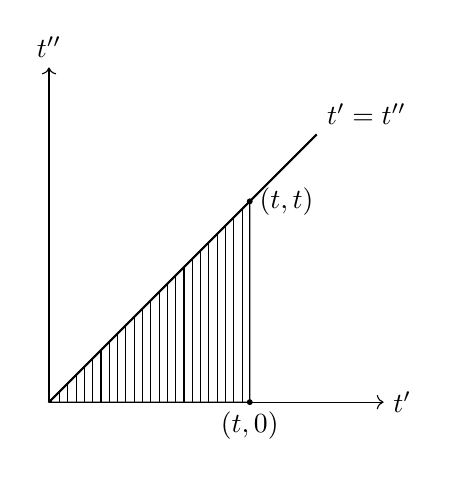
\begin{tikzpicture}[scale=0.85]
            % axes
            \draw[->] (0,0) -- (5,0) node[right] {$t'$};
            \draw[->] (0,0) -- (0,5) node[above] {$t''$};
            % t'=t'' line
            \draw[thick] (0,0) -- (4,4) node[above right] {$t'=t''$};
            % define base length t (adjust as needed)
            \def\t{3}
            % shaded triangle using vertical line pattern
            \draw[pattern=vertical lines,pattern color=black] (0,0) -- (\t,0) -- (\t,\t) -- cycle;
            % optional: mark point at (t,0) and (t,t)
            \filldraw (\t,0) circle (1pt) node[below] {$(t,0)$};
            \filldraw (\t,\t) circle (1pt) node[right] {$(t,t)$};
        \end{tikzpicture}
    \end{figure}

    We can also have the \(t''\) integration to go from \(0\) to \(t\), since we are explicitly enforcing time ordering, we will get the same expression but twice. (Think carefully about this, if there were no time ordering, this manipulation would not be possible, since for the upper triangle, we would be having the products wrongly ordered. The presence of time ordering allows one to extend the integral without altering its value.) Similarly, we can extend all the integrals to \(t\), while being reassured by the time ordering that we are getting consistent results, while dividing by \(n!\) which removes the factor of adding over all the possible arrangements of the \(n\) dummy variables. Therefore, we can write the above also as 
    \begin{equation*}
        U_I(t) = 1 - i\int_0^t T(H(t')) dt' + (-i)^2 \frac{1}{2!}\int_0^t \int_0^t T(H(t')H(t''))dt''dt' + \cdots
    \end{equation*}

    \textcolor{red}{
        Let us again explicitly see this in the case of the discrete sum 
        which now would be rewritten as 
        \begin{equation*}
            \sum_0^t \sum_0^t T(H(a) H(b))
        \end{equation*}
        This would be equal to 
        \begin{align*}
            &\sum_{a>b} H(a)H(b) + \sum_{a<b}H(b)H(a) + \sum_{a=b}H(a)^2
        \end{align*}
        Since the first two sums are equal, we get 
        \begin{equation*}
            2\sum_{a>b} H(a)H(b) + \sum_{a=b}H(a)^2
        \end{equation*}
        In continuum, the diagonal term has zero measure and drops out, and therefore, we will be left with twice the intended integral as expected.\\
    }

    Therefore 
    \begin{equation*}
        U_I(t) = \sum_{n=0}^\infty \frac{(-i)^n}{n!} \left(\int_0^t\right)^n T(H(t_1) H(t_2) \cdots H(t_n)) ~dt_1 dt_2 \cdots dt_n 
    \end{equation*}
    and there is a formal way to write this, called the Dyson's formula
    \begin{equation*}
        U_I(t) = T\left\{ \e^{-i\int_0^t H_I(t')dt'}  \right\}
    \end{equation*}
    What this means is that we expand the exponential in its Taylor series and then apply the time ordering to very term.\\

    Given an operator in terms of the free fields \(\phi_I(t,\textbf{x})\), the above derived \(U_I(t)\) gives us a way to obtain the full Heisenberg picture operators. An inherent advantage is that this formula is already in the form of a power series in \(H_I\), and therefore naturally provides a perturbative series.

    \newpage
    \section{Wick's Theorem}
    In general, what we want to compute is what the matrix elements of the above derived \(U_I(t)\) are, since this gives us the amplitudes for some in states going to some out states. In computing these matrix elements, we have to compute the matrix elements of the kind 
    \begin{equation*}
        \braket{\psi_1 | T[H_I(t_1),\cdots,H_I(t_n)]|\psi_2}
    \end{equation*}
    where \(\ket{\psi_1}\) and \(\ket{\psi_2}\) are the in and out states (we will later formulate these only in terms of vacuum expectation values, but it is more physically relevant to talk about these matrix elements). Once we know all these elements, we can sum them according to the Dyson's formula to get the matrix element of \(U_I\) which gives us the \(S-\)matrix. \\

    The \(H_I(t)\) is some polynomial in \(\phi_I(t, \textbf{x})\), and therefore, the above expectation values reduce to calculating elements of the form 
    \begin{equation*}
        \braket{\psi_1 | T[\phi_I(x_1),\cdots,\phi_I(x_n)]|\psi_2}
    \end{equation*}

    Remember that the interaction picture fields are simply
    \begin{equation*}
        \phi_I(t,\textbf{x}) = \int \a{p}\e^{-ip\cdot x} + \adag{p}\e^{ip\cdot x} \frac{d^3\textbf{p}}{(2\pi)^3 \sqrt{2\w_\textbf{p}}}
    \end{equation*}
    and the above matrix values are simply matrix elements of the time ordered products of the fields of this kind. But see that the time ordered product is going to be a mess, to see why consider a simple case of three field insertions 
    \begin{align*}
        T[\phi(x_1)\phi(x_2)\phi(x_3)] =& ~\theta(x_1^0 - x_2^0)\theta(x_1^0 - x_3^0)\theta(x_2^0 - x_3^0) \phi(x_1)\phi(x_2)\phi(x_3) \\
        &+  \theta(x_2^0 - x_1^0)\theta(x_2^0 - x_3^0)\theta(x_1^0 - x_3^0) \phi(x_2)\phi(x_1)\phi(x_3) \\
        &+ \text{ 4 other terms}
    \end{align*}
    Each of the term above has further \(2^3\) terms since each field insertion has a creation and annihilation operator, and therefore the product of \(n\) such field insertions has \(2^n\) terms. This expression only gets more complicated for polynomials with more field insertions, which is natural in such interaction Hamiltonians, and therefore the entire matrix element is a mess. The tool that is used to simplify this mess is called the Wick's theorem.

    \subsection{Contractions}

    Earlier, we had encountered the normal ordering, which was simply an instruction to place all the annihilation operators on the right. We can extend this definition to the interaction picture field operators by expanding them in terms of creation and annihilation operators and normal order it. That is, 
    \begin{equation*}
        \phi_I(x) = \phi_I^+(x) + \phi_I^-(x)
    \end{equation*}
    where 
    \begin{equation*}
        \phi_I^+(x) = \int \a{p}\e^{-ip\cdot x} \frac{d^3\textbf{p}}{(2\pi)^3 \sqrt{2\w_\textbf{p}}}~~~~\&~~~~\phi_I^-(x) = \int \adag{p}\e^{ip\cdot x} \frac{d^3\textbf{p}}{(2\pi)^3 \sqrt{2\w_\textbf{p}}}
    \end{equation*}
    (which is taken by convention — positive frequency contains the annihilation operators and negative frequency contains the creation operators) then, 
    \begin{align*}
        \normord{\phi_I(x_1) \phi_I(x_2)} &= \normord{\phi_I^+(x_1)\phi_I^+(x_2)} + \normord{\phi_I^+(x_1)\phi_I^-(x_2)} + \normord{\phi_I^-(x_1)\phi_I^+(x_2)} + \normord{\phi_I^-(x_1)\phi_I^-(x_2)}\\
        &= \phi_I^+(x_1)\phi_I^+(x_2) + \phi_I^-(x_2)\phi_I^+(x_1) + \phi_I^-(x_1)\phi_I^+(x_2) + \phi_I^-(x_1)\phi_I^-(x_2)
    \end{align*}
    (where only the second term is different from the regular product)
    Notice that normal ordered product is NOT defined for operators in Heisenberg picture since in Heisrnberg picture in the presence of interactions, there is no splitting of the field into creation and annihilation operators. This ordering is only valid for interactin picture fields\\

    We define a contraction as 
    \begin{equation*}
        \wick{\c \phi_I(x_1) \c \phi_I(x_2)} = T[\phi_I(x_1) \phi_I(x_2)] - \normord{\phi_I(x_1) \phi_I(x_2)}
    \end{equation*}
    The normal ordered product and time ordered product are operators, but contraction is just a number. We know that 
    \begin{equation*}
        T[\phi_I(x_1) \phi_I(x_2)] = \theta(x_1^0 - x_2^0) \phi_I(x_1) \phi_I(x_2) + \theta(x_2^0 - x_1^0) \phi_I(x_2) \phi_I(x_1)
    \end{equation*}
    and the normal ordered product is 
    \begin{equation*}
        \normord{\phi_I(x_1) \phi_I(x_2)} = \phi_I^+(x_1)\phi_I^+(x_2) + \phi_I^-(x_2)\phi_I^+(x_1) + \phi_I^-(x_1)\phi_I^+(x_2) + \phi_I^-(x_1)\phi_I^-(x_2)
    \end{equation*}
    we can simply insert a \(\theta\) function in the normal ordered product without altering it as 
    \begin{align*}
        \normord{\phi_I(x_1) \phi_I(x_2)} =& \theta(x_1^0 - x_2^0)\left[ \phi_I^+(x_1)\phi_I^+(x_2) + \phi_I^-(x_2)\phi_I^+(x_1) + \phi_I^-(x_1)\phi_I^+(x_2) + \phi_I^-(x_1)\phi_I^-(x_2) \right] \\
         &+ \theta(x_2^0 - x_1^0)\left[ \phi_I^+(x_1)\phi_I^+(x_2) + \phi_I^-(x_2)\phi_I^+(x_1) + \phi_I^-(x_1)\phi_I^+(x_2) + \phi_I^-(x_1)\phi_I^-(x_2) \right]
    \end{align*}
    Then the difference in the two products would be (noticing that the only different term is the second term in the normal ordering)
    \begin{align*}
        \wick{\c \phi_I(x_1) \c \phi_I(x_2)} &= \theta(x_1^0 - x_2^0)\left( \phi_I^+(x_1)\phi_I^-(x_2) - \phi_I^-(x_2)\phi_I^+(x_1) \right) + \theta(x_2^0 - x_1^0) \left(  \phi_I^+(x_2)\phi_I^-(x_1) - \phi_I^-(x_1)\phi_I^+(x_2)  \right)\\
        &=\theta(x_1^0 - x_2^0) [\phi_I^+(x_1), \phi_I^-(x_2)] + \theta(x_2^0 - x_1^0) [\phi_I^+(x_2), \phi_I^-(x_1)] 
    \end{align*}
    These commutators are only numbers, and not operators.

    \subsection{The theorem}

    Wick's theorem simply tell that 
    
    \begin{equation}
            \begin{split}
                T[\phi_I(x_1) \phi_I(x_2)& \cdots \phi_I(x_n)] = \normord{\phi_I(x_1) \phi_I(x_2) \cdots \phi_I(x_n)} + \normord{\wick{\c \phi_I(x_1) \c \phi_I(x_2)} \cdots \phi_I(x_n)} \\
                &+ \normord{\wick{\c \phi_I(x_1) \phi_I(x_2)\c \phi_I(x_3)} \cdots \phi_I(x_n)} + \text{ other terms with 1 contraction}\\
                &+ \normord{\wick{\c1 \phi_I(x_1) \c1 \phi_I(x_2) \c1 \phi_I(x_3) \c1 \phi_I(x_4)} \cdots \phi_I(x_n)} + \text{ other terms with 2 contractions}\\
                &+ \cdots \text{ terms with 3 and more contractions}\\
                &+ \begin{cases}
                    \normord{\wick{\c1 \phi_I(x_1) \c1 \phi_I(x_2) \cdots \c1 \phi_I(x_{n-2}) \c1 \phi_I(x_{n-1})} \phi_I(x_n)} + \text{terms with only one uncontracted field } : n \text{ odd}\\
                    \normord{\wick{\c1 \phi_I(x_1) \c1 \phi_I(x_2) \cdots \c1 \phi_I(x_{n-1}) \c1 \phi_I(x_{n})}} + \text{terms with no uncontracted field } : n \text{ even}
                \end{cases}
            \end{split}
            \label{eq:wick}
    \end{equation}
    As an example, 
    \begin{align*}
        T[\phi_I(x_1) \phi_I(x_2) \phi_I(x_3)\phi_I(x_4)] =& \normord{\phi_I(x_1) \phi_I(x_2) \phi_I(x_3)\phi_I(x_4)} + \normord{\wick{\c\phi_I(x_1) \c\phi_I(x_2) \phi_I(x_3)\phi_I(x_4)}}\\
        &+\normord{\wick{\c\phi_I(x_1) \phi_I(x_2)\c \phi_I(x_3)\phi_I(x_4)}} + \normord{\wick{\c\phi_I(x_1)\phi_I(x_2) \phi_I(x_3)\c\phi_I(x_4)}}\\
        &+\normord{\wick{\phi_I(x_1) \c\phi_I(x_2) \c\phi_I(x_3)\phi_I(x_4)}}+\normord{\wick{\phi_I(x_1) \c\phi_I(x_2) \phi_I(x_3)\c\phi_I(x_4)}}\\
        &+\normord{\wick{\phi_I(x_1) \phi_I(x_2) \c\phi_I(x_3) \c\phi_I(x_4)}} + \normord{\wick{\c \phi_I(x_1) \c \phi_I(x_2) \c\phi_I(x_3) \c\phi_I(x_4)}} \\
        &+\normord{\wick{\c\phi_I(x_1) \c2\phi_I(x_2) \c\phi_I(x_3) \c2\phi_I(x_4)}}
    \end{align*}

    \underline{Proof}\\
    We prove the theorem by induction.\\
    For \(n=2\), the theorem is definitely true, by the definition of contraction.\\
    Suppose the theorem is true for some \(n\). That is 
    \begin{equation*}
        T[\phi_I(x_1)\cdots\phi_I(x_n)] = W(x_1, \cdots, x_n)
    \end{equation*}
    where we used \(W\) as the shorthand for the RHS in equation (\ref{eq:wick})\\
    For \(n+1\), let us assume without loss of generality that \(x_1^0\) is the latest time. We can do this because inside the \(T\) all operators commute, since at the end \(T\) rearranges them according to their time ordering, and therefore, we can bring the field with the latest time to the first and call it \(\phi_I(x_1)\). Then 
    \begin{equation*}
        T(\phi_I(x_1)\phi_I(x_2) \cdots \phi_I(x_{n+1})) = \phi_I(x_1)T(\phi_I(x_2) \cdots \phi_I(x_{n+1})) 
    \end{equation*}
    From our assumption that the theorem is true for \(n\), \(T(\phi_I(x_2) \cdots \phi_I(x_{n+1}) )= W(x_2, \cdots x_{n+1})\). Now 
    \begin{equation*}
        \phi_I(x_1) = \phi_I^+(x_1) + \phi_I^-(x_1)
    \end{equation*} 
    which means 
    \begin{equation*}
        T(\phi_I(x_1)\phi_I(x_2) \cdots \phi_I(x_{n+1})) = (\phi_I^-(x_1) + \phi_I^+(x_1))W(x_2, \cdots x_{n+1}) 
    \end{equation*}
    The first term in the RHS is already has \(\phi^-\) on the left, but the second term is not normal ordered. Therefore, we can commute the \(\phi^+\) to normal order the second term too as
    \begin{equation*}
        T(\phi_I(x_1)\phi_I(x_2) \cdots \phi_I(x_{n+1})) = \phi_I^-(x_1)W(x_2, \cdots x_{n+1}) + W(x_2, \cdots x_{n+1})\phi_I^+(x_1) + [\phi_I^+(x_1), ~W(x_2, \cdots x_{n+1})]
    \end{equation*} 
    The first two terms when added together simply gives 
    \begin{equation*}
        \normord{\phi_I(x_1) W(x_2, \cdots x_{n+1})}
    \end{equation*}
    which is the set of \(\normord{\phi_I(x_1) \phi_I(x_2) \cdots \phi_I(x_{n+1})}\) and all terms with \(\phi_I(x_1)\) uncontracted. \\

    The next part, which is the commutator, will have terms of the form 
    \begin{equation*}
        [\phi_I^+(x_1), \phi_I(x_m)] = [\phi_I^+(x_1), \phi^-_I(x_m)]~ \because \phi^+\text{ at different spacetime points commute}
    \end{equation*}
    But since \(x_1^0 > x_m^0\forall m\), we can also rewrite this as
    \begin{equation*}
        \theta(x_1^0 - x_m^0)[\phi_I^+(x_1), \phi^-_I(x_m)] + \theta(x_m^0 - x_1^0)[\phi_I^+(x_m), \phi^-_I(x_1)] = \wick{\c\phi_I(x_1) \c\phi_I(x_m)}
    \end{equation*} 
    Therefore, the second part will have contractions of \(\phi_I(x_1)\) with all \(\phi_I(x_m)\). \\

    The sum of the first and second part will have everything that is required in \(W(x_1, \cdots, x_{n+1})\), i.e.\ there is a normal ordered product, plus all possible contractions of all fields. Therefore, for \(n+1\)
    \begin{equation*}
        T(\phi_I(x_1)\phi_I(x_2) \cdots \phi_I(x_{n+1})) = W(x_1, \cdots, x_{n+1})
    \end{equation*}
    Therefore, Wick's theorem is proved by mathematical induction.\\

    What makes Wick's theorem useful, and therefore significant, is that it makes evaluation of these time ordered products simple. Suppose we were calculating the vacuum expectation values of a given \(T(\phi_I(x_1)\cdots\phi_I(x_n))\). The only contribution would be from the terms where all the fields are contracted, since other terms are normal ordered and normal ordered products annihilate vacuum and therefore have zero vacuum expectation values. 

    \subsection{The Feynman Propagator}
    See that 
    \begin{equation*}
        \braket{0|T(\phi_I(x) \phi_I(y))|0} = \braket{0|\wick{\c \phi_I(x) \c \phi_I(y)} |0} = \wick{\c \phi_I(x) \c \phi_I(y)} 
    \end{equation*}
    Since the normal ordered product annihilates the vacuum, contraction is a number, and \(\braket{0|0} = 1\).\\

    For \(x^0 > y^0\), this evaluates to 
    \begin{equation*}
        \int \bra{0} \a{q} \e^{-iq\cdot x} \adag{p}\e^{ip\cdot y} \ket{0} \frac{d^3\textbf{p}d^3\textbf{q}}{(2\pi)^6 2\sqrt{\w_\textbf{p}\w_\textbf{q}}}
    \end{equation*}
    since all other terms give zero. We can now commute the \(a\) and \(\adag{}\) to get a delta function, which removes one integral in \(\textbf{q}\), and obtain 
    \begin{equation*}
        \int \e^{-ip\cdot(x-y)}\frac{1}{2\w_\textbf{p}} \frac{d^3\textbf{p}}{(2\pi)^3}
    \end{equation*}
    When \(y^0 > x^0\), we similarly get 
    \begin{equation*}
        \int \e^{ip\cdot(x-y)}\frac{1}{2\w_\textbf{p}} \frac{d^3\textbf{p}}{(2\pi)^3}
    \end{equation*}
    and therefore the contraction looks like 
    \begin{equation}
        \wick{\c \phi_I(x) \c \phi_I(y)} = \theta(x^0 - y^0) \int \e^{-ip\cdot(x-y)}\frac{1}{2\w_\textbf{p}} \frac{d^3\textbf{p}}{(2\pi)^3} ~~+~~\theta(y^0-x^0) \int \e^{ip\cdot(x-y)}\frac{1}{2\w_\textbf{p}} \frac{d^3\textbf{p}}{(2\pi)^3}
        \label{eq:contraction-full}
    \end{equation}

    We can write it in a slighly simpler way as 
    \begin{equation}
        \wick{\c \phi_I(x) \c \phi_I(y)}  = \int\frac{i}{p^2 - m^2 + i\epsilon} \e^{-ip\cdot(x-y)}\frac{d^4p}{(2\pi)^4} = \int \e^{-ip_0 (x^0 - y^0)} \e^{i\textbf{p}\cdot (\textbf{x}- \textbf{y})} \frac{i}{p_0^2 - \textbf{p}^2 - m^2 + i\epsilon} \frac{dp_0 d^3\textbf{p}}{(2\pi)^4}
        \label{eq:feynman}
    \end{equation}
    The \(i\epsilon\) is just a prescription to indicate in which direction the contour should be closed. See that when we do the integral over \(p_0\) without the \(i\epsilon\) shifting, it has two poles, 
    \begin{equation*}
        p_0^2 - \textbf{p}^2 - m^2 = 0 \implies p_0 = \pm \w_\textbf{p}
    \end{equation*}
    on the real axis and therefore the integral is ill defined. The \(i\epsilon\) shifts the poles in such a way that taking a contour along the real axis and closing the contour along one of the two half planes will give the correct result.\\


    With the introduction of \(i\epsilon\), the poles now move to 
    \begin{equation*}
        p_0 = \pm \sqrt{\w_\textbf{p}^2 - i\epsilon} \approx \pm \left( \w_\textbf{p} - \frac{i\epsilon}{2\w_\textbf{p}} \right) \approx \pm (\w_\textbf{p} - i\epsilon)
    \end{equation*}
    (notice that the \(i\epsilon\) is simply an integral prescription and its value has no meaning). Therefore, for the \(p_0\) integral the location of poles is shown in figure (\ref{fig:prescription})
    \begin{figure}[h]
        \centering
        \begin{tikzpicture}[>=latex, scale=1]
            \draw[->] (-3,0) -- (3,0);
            \draw[->] (0, -1.5) -- (0,1.5);
            \fill (1.5,0) circle (2pt);
            \node at (-1.5, -0.25) {\(-\w_\textbf{p}\)};
            \node at (1.5, 0.25) {\(\w_\textbf{p}\)};
            \fill (-1.5,0) circle (2pt);

            \node at (1.5, -1.2) {\(\w_\textbf{p} - i\epsilon\)};
            \node at (1.5, -0.75) {\(\mathsf{X}\)};
            \node at (-1.5, 1.2) {\(-\w_\textbf{p} + i\epsilon\)};
            \node at (-1.5, 0.75) {\(\mathsf{X}\)};

            \begin{scope}[xshift=7cm]
                \draw[->, opacity=0.35] (-3,0) -- (3,0);
                \draw[->, opacity=0.35] (0, -1.5) -- (0,1.5);
                \fill (1.5,0) circle (2pt);
                \node at (-1.5, 0.25) {\(-\w_\textbf{p}\)};
                \node at (1.5, -0.25) {\(\w_\textbf{p}\)};
                \fill (-1.5,0) circle (2pt);
                \draw[->] (1,0) arc (180:0:0.5);
                \draw[<-] (-1,0) arc (360:180:0.5);
                \draw[->] (-1,0) -- (1,0);
                \draw (2,0) -- (3,0);
                \draw (-2,0) -- (-3,0);
            \end{scope}
        \end{tikzpicture}
        \caption{The position of poles in case of \(i\epsilon\) prescription (left), and the equivalent contour we need to consider when working without the shifting (right)}\label{fig:prescription}
    \end{figure}

    To check that this expression with this pole prescription gives the correct result, consider the two cases\\

    1.\ \(x_0 > y_0\)\\
    The integrand is 
    \begin{equation*}
        \e^{-ip_0(x^0 - y^0)} = \e^{-i\mathrm{Re}(p_0) (x^0 - y^0)}\e^{\mathrm{Im}(p_0)(x^0 - y^0)}
    \end{equation*}
    In the upper half of the complex plane, this blows at \(|p_0| \to \infty\) and therefore we close the contour in lower half of the complex plane, picking up the pole at \(\w_\textbf{p} - i\epsilon\). The contour is closed in clockwise sense and the value of the integral is  
    \begin{equation*}
        -2\pi i\frac{1}{2\w_\textbf{p}}\e^{-i\w_\textbf{p}(x^0 - y^0)}
    \end{equation*}
    When plugging the value of this integral into the equation (\ref{eq:feynman}) where one factor of \(2\pi\) cancels with the \((2\pi)^4\) in denominator, and \(-i\) multiplies with \(i\) to give \(1\), we get 
    \begin{equation*}
        \int \e^{-ip\cdot(x-y)}\frac{1}{2\w_\textbf{p}} \frac{d^3\textbf{p}}{(2\pi)^3}
    \end{equation*}
    
    2.\ \(x_0 < y_0\)\\
    In this case the integrand is zero at infinity in the upper half plane and therefore we complete the contour in the upper half plane, picking up the pole at \(p_0 = -\w_\textbf{p}\). The contour is closed counterclockwise, and therefore the integral is 
    \begin{equation*}
        (2\pi i)(-1)\frac{1}{2\w_\textbf{p}}\e^{i\w_\textbf{p}(x^0 - y^0)}
    \end{equation*}
    Plugging this back, we get 
    \begin{equation*}
        \int \e^{i\w_\textbf{p}\cdot(x_0-y_0) + i\textbf{p}\cdot(\textbf{x} - \textbf{y})}\frac{1}{2\w_\textbf{p}} \frac{d^3\textbf{p}}{(2\pi)^3}
    \end{equation*}
    We can convert the integral from \(\textbf{p}\) to \(-\textbf{p}\) to get 

    \begin{equation*}
        \int \e^{ip\cdot(x-y)}\frac{1}{2\w_\textbf{p}} \frac{d^3\textbf{p}}{(2\pi)^3}
    \end{equation*}

    Therefore we recover
    \begin{equation*}
        \wick{\c \phi_I(x) \c \phi_I(y)} = G_F(x-y) =  \begin{cases}
            \displaystyle\int \e^{-ip\cdot(x-y)}\frac{1}{2\w_\textbf{p}} \frac{d^3\textbf{p}}{(2\pi)^3} &: x_0 > y_0\\
            \displaystyle\int \e^{ip\cdot(x-y)}\frac{1}{2\w_\textbf{p}} \frac{d^3\textbf{p}}{(2\pi)^3} &: x_0 < y_0
        \end{cases}
    \end{equation*}
    as required. This is called the Feynman Green's function (Feynman Propagator). (Notice that it was very important to consider \(+i\epsilon\) in the denominator. Any other addition would not give this result.)\\

    There is another way to understand this \(i\epsilon\) prescription as 
    \begin{equation*}
        \frac{1}{x - a - i\epsilon} = P\left( \frac{1}{x-a} \right) + i\pi \delta(x-a)
    \end{equation*}
    where \(P()\) stands for the principle value. The above equation is, in essence, a distribution valued equation, and it makes sense only under an integral 
    \begin{equation*}
        \int \frac{f(x)}{x-a-i\epsilon} dx = P\int \frac{f(x)}{x-a} dx + i\pi f(a) =\lim_{\delta \to 0} \left(\int_{-\infty}^{a-\delta} \frac{f(x)}{x-a} dx+ \int_{a+\delta}^{\infty} \frac{f(x)}{x-a} dx \right) + i\pi f(a)
    \end{equation*}

    To prove this, let us consider the equation
    \begin{equation*}
        \frac{1}{x-a-i\epsilon} - \frac{1}{x-a+i\epsilon} = 2i\pi\delta(x-a)
    \end{equation*}
    which we obtained from adding the above equation to its complex conjugate.\\
    This is equivalent to stating that 
    \begin{equation*}
        \int dx \frac{f(x)}{x-a-i\epsilon} - \int dx \frac{f(x)}{x-a+i\epsilon} = 2i\pi f(a)
    \end{equation*}

    The first term in the above equation simply implies the choice of the contour 
    \begin{figure}[h]
        \centering
        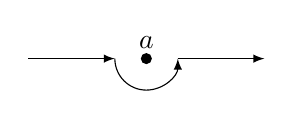
\begin{tikzpicture}[>=latex, scale=1]
            \draw[->] (-1.5, 0) -- (-0.4,0);
            \draw[<-] (1.5, 0) -- (0.4,0);
            \draw[->] (-0.4,0) arc (180:360:0.4);
            \fill (0,0) circle (2pt);
            \node at (0,0.2) {\(a\)};
        \end{tikzpicture}
    \end{figure}

    and the second term implies the choice of the contour 
    \begin{figure}[h]
        \centering
        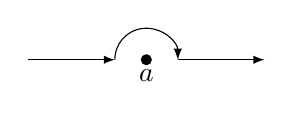
\begin{tikzpicture}[>=latex, scale=1]
            \draw[->] (-1.5, 0) -- (-0.4,0);
            \draw[<-] (1.5, 0) -- (0.4,0);
            \draw[->] (-0.4,0) arc (180:0:0.4);
            \fill (0,0) circle (2pt);
            \node at (0,-0.2) {\(a\)};
        \end{tikzpicture}
    \end{figure}

    Subtracting the above two is equivalent to reversing the direction of the second contour and adding, in which case the only piece that remains is 
    \begin{figure}[h]
        \centering
        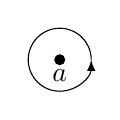
\begin{tikzpicture}[>=latex, scale=1]
            \draw[->] (0.4,0) arc (0:360:0.4);
            \fill (0,0) circle (2pt);
            \node at (0,-0.2) {\(a\)};
        \end{tikzpicture}
    \end{figure}

    which is equal to \(2\pi i\) times the residue of the function at \(x=a\), which is exactly equal to \(2\pi i f(a)\).\\

    Notice that the Feynman progagator also satisfies 
    \begin{equation*}
        (\square + m^2) \braket{0|T(\phi_I(x) \phi_I(y))|0} = -i\delta^4(x-y)
    \end{equation*}

    \textcolor{red}{
        \begin{align*}
                \braket{0|T(\phi_I(x) \phi_I(y))|0} &= \int\frac{i}{p^2 - m^2 + i\epsilon} \e^{-ip\cdot(x-y)}\frac{d^4p}{(2\pi)^4} \\
                \implies (\square + m^2) \braket{0|T(\phi_I(x) \phi_I(y))|0} &= (\square + m^2) \int\frac{i}{p^2 - m^2 + i\epsilon} \e^{-ip\cdot(x-y)}\frac{d^4p}{(2\pi)^4} \\
                &= \int \frac{i}{p^2 - m^2 + i\epsilon} ((-ip)^2 + m^2) \e^{-ip\cdot(x-y)}\frac{d^4p}{(2\pi)^4}\\
                &= -i \int \e^{-ip\cdot(x-y)}\frac{d^4p}{(2\pi)^4}\\
                &= -i\delta^4(x-y)
        \end{align*}
    }
    
    The Feynman propagator has the property that it propagates positive frequencies forward in time, and negative frequencies backwards in time. To see what this means, see that from equation (\ref{eq:contraction-full}), we see that the Feynman propagator is of the form 
    \begin{equation*}
        \int \theta(x^0 - y^0)  \e^{-ik\cdot (x-y)} \theta(k^0) f(k) \frac{d^4k}{(2\pi)^4}  + \int \theta(y^0 - x^0)  \e^{-ik\cdot (x-y)} \theta(-k^0) f(k) \frac{d^4k}{(2\pi)^4}
    \end{equation*}
    (where \(f(k)\) is the \(delta(k^2 - m^2)\), and in the above equation we have simply taken equation (\ref{eq:contraction-full}) and converted it into a manifestly Lorentz invarent \(4-\)integral).\\
    In the second integral, rather than writing the conversion as \(\e^{ik\cdot(x-y)} \theta(k^0) f(k)\), we wrote it as \(\e^{-ik\cdot(x-y)}\theta(-k^0)f(k)\) and used the invariance of the \(3-\)integral under \(\textbf{k}\to -\textbf{k}\). \\
    The propagator in this form has the combinations \(\theta(x^0 - y^0)\theta(k^0)\) and \(\theta(y^0 - x^0)\theta(-k^0)\) which imply that the Feynman propagator propagates positive frequencies forward in time and negative frequencies backward in time.\\

    Feynman propagator is one kind of propagator. We could have considered an anti-time ordered propagator, which would come with a \(-i\epsilon\), and would have the opposite baheviour, propagating positive frequencies backward in time and negative frequencies forward in time. Then there are other propagators which send both the frequencies either backwards or forwards.

    \subsection{The retarded propagator}
    The retarded propagator is simply 
    \begin{equation*}
        \theta(x^0 - y^0)\bra{0}[\phi_I(x), \phi_I(y) ]\ket{0} = G_R(x-y)
    \end{equation*}
    Notice that this propagator also satisfies 
    \begin{equation*}
        (\square + m^2)G_R(x-y) = -i\delta^4(x-y)
    \end{equation*}
    This implies that \(G_F\) and \(G_R\) should differ by only a solution of the equation of motion. To check that this is true, notice that 
    \begin{equation*}
        \frac{\del}{\del x^0} \left(\theta(x^0 - y^0)\bra{0}[\phi_I(x), \phi_I(y) ]\ket{0}\right) = \delta(x^0 - y^0)\bra{0}[\phi_I(x), \phi_I(y) ]\ket{0} + \theta(x^0 - y^0)\frac{\del}{\del x^0} \bra{0}[\phi_I(x), \phi_I(y) ]\ket{0}
    \end{equation*}
    The first term is zero, since at equal times, the fields commute and the delta function enforces equal time. 
    Therefore we get 
    \begin{equation*}
        \frac{\del}{\del x^0} \left(\theta(x^0 - y^0)\bra{0}[\phi_I(x), \phi_I(y) ]\ket{0}\right) = \theta(x^0 - y^0) \bra{0}[\dot{\phi}_I(x), \phi_I(y) ]\ket{0}
    \end{equation*}
    The second derivative w.r.to \(x^0\) would therefore be 
    \begin{align*}
        \frac{\del^2}{\del (x^0)^2} \left(\theta(x^0 - y^0)\bra{0}[\phi_I(x), \phi_I(y) ]\ket{0}\right) &= \delta(x^0 - y^0) \bra{0}[\Pi_I(x), \phi_I(y) ]\ket{0} + \theta(x^0 - y^0) \bra{0}[\ddot{\phi}_I(x), \phi_I(y) ]\ket{0} \\
        &= -i\delta(x^0 - y^0)\delta^3(\textbf{x} - \textbf{y}) + \theta(x^0 - y^0) \bra{0}[\ddot{\phi}_I(x), \phi_I(y) ]\ket{0} 
    \end{align*}
    where in the first term the delta function imposed equal times, and therefore the commutator becomes simply an equal time commutation relation. \\

    There are other terms which are \((-\nabla_x^2 + m^2) G_R\). The \(\nabla_x\) doesn't care about the \(\theta\) function and therefore we would simply get 
    \begin{equation*}
        (-\nabla_x^2 + m^2) \left(\theta(x^0 - y^0)\bra{0}[\phi_I(x), \phi_I(y) ]\ket{0}\right) = \theta(x^0 - y^0)\bra{0}[(-\nabla_x^2 + m^2)\phi_I(x), \phi_I(y) ]\ket{0}
    \end{equation*}
    Adding this and the above equation, we see that we get 
    \begin{equation*}
        (\square + m^2)\left(\theta(x^0 - y^0)\bra{0}[\phi_I(x), \phi_I(y) ]\ket{0}\right) = -i\delta(x^0 - y^0)\delta^3(\textbf{x} - \textbf{y}) + \theta(x^0 - y^0) \bra{0}[(\square + m^2)\phi_I(x), \phi_I(y) ]\ket{0}
    \end{equation*}
    But since \((\square + m^2)\phi_I(x) = 0\), we get 
    \begin{equation*}
        (\square + m^2)\left(\theta(x^0 - y^0)\bra{0}[\phi_I(x), \phi_I(y) ]\ket{0}\right) = -i\delta(x^0 - y^0)\delta^3(\textbf{x} - \textbf{y}) = -i\delta^4(x-y)
    \end{equation*}

    Let us try evaluating this expression in momentum space, the propagator becomes 
    \begin{align*}
        \theta(x^0 - y^0)[\phi_I(x), \phi_I(y)] &= \int \left(  [\a{q}, \adag{p}] \e^{-iq\cdot x + ip\cdot y} + [\adag{q}, \a{p}]\e^{iq\cdot x - ip\cdot y}  \right)\frac{d^3\textbf{p}d^3\textbf{q}}{(2\pi)^62\sqrt{\w_\textbf{p}\w_\textbf{q}}}\\
        &= \int \e^{-iq\cdot(x-y)} - \e^{iq\cdot (x-y)} \frac{d^3\textbf{q}}{(2\pi)^32\w_\textbf{q}}\theta(x^0 - y^0)
    \end{align*}
    Claim - the whole retarded propagator can be written as 
    \begin{equation*}
        G_R(x-y) = \int \frac{i}{(k_0 + i\epsilon)^2 - \textbf{k}^2 - m^2} \e^{-ik\cdot(x-y)} \frac{d^4k}{(2\pi)^4}
    \end{equation*}
    In this case, the poles are at \(k^0 = \pm \w_\textbf{k} - i\epsilon\).

    \begin{figure}[h]
        \centering
        \begin{tikzpicture}[>=latex, scale=1]
            \draw[->] (-3,0) -- (3,0);
            \draw[->] (0, -1.5) -- (0,1.5);
            \fill (1.5,0) circle (2pt);
            \node at (-1.5, 0.25) {\(-\w_\textbf{k}\)};
            \node at (1.5, 0.25) {\(\w_\textbf{k}\)};
            \fill (-1.5,0) circle (2pt);

            \node at (1.5, -1.2) {\(\w_\textbf{p} - i\epsilon\)};
            \node at (1.5, -0.75) {\(\mathsf{X}\)};
            \node at (-1.5, -1.2) {\(-\w_\textbf{p} + i\epsilon\)};
            \node at (-1.5, -0.75) {\(\mathsf{X}\)};

            \begin{scope}[xshift=7cm]
                \draw[->, opacity=0.35] (-3,0) -- (3,0);
                \draw[->, opacity=0.35] (0, -1.5) -- (0,1.5);
                \fill (1.5,0) circle (2pt);
                \node at (-1.5, -0.25) {\(-\w_\textbf{p}\)};
                \node at (1.5, -0.25) {\(\w_\textbf{p}\)};
                \fill (-1.5,0) circle (2pt);
                \draw[->] (1,0) arc (180:0:0.5);
                \draw[->] (-2,0) arc (180:0:0.5);
                \draw[->] (-1,0) -- (1,0);
                \draw (2,0) -- (3,0);
                \draw (-2,0) -- (-3,0);
            \end{scope}
        \end{tikzpicture}
        \caption{The position of the shifted poles (left), and the equivalent contour (right).}
    \end{figure}
    
    For \(x^0 < y^0\), we need to close the contour in the upper half plane, where it does not enclose any poles. Therefore the integral is zero. \\

    For \(x^0 > y^0\), we close the contour in the lower half plane, picking up residues of both the poles. The residues are the same as we had calculated for the case of Feynman propagator, and therefore the above integral for \(x^0 > y^0\) becomes
    \begin{equation*}
        (-2\pi i ) \frac{i}{2\pi} \left(\int \e^{-ik\cdot(x-y)}\frac{1}{2\w_\textbf{k}} \frac{d^3\textbf{k}}{(2\pi)^3} + \int \e^{ik\cdot(x-y)}\frac{1}{-2\w_\textbf{k}} \frac{d^3\textbf{k}}{(2\pi)^3} \right)
    \end{equation*}
    therefore giving 
    \begin{equation*}
        G_R(x-y) = \int \frac{i}{(k_0 + i\epsilon)^2 - \textbf{k}^2 - m^2} \e^{-ik\cdot(x-y)} \frac{d^4k}{(2\pi)^4} = \theta(x^0 - y^0) \int \e^{-ik\cdot(x-y)}\frac{1}{2\w_\textbf{k}} {(2\pi)^3} - \e^{ik\cdot(x-y)}\frac{1}{2\w_\textbf{k}} \frac{d^3\textbf{k}}{(2\pi)^3}
    \end{equation*}
    as required.\\

    There is also an advanced propagator, with \(\theta(y^0-x^0)\) and for this case the pole prescription would be \((k_0 + i\epsilon)^2 - \textbf{k}^2 - m^2\).\\

    The retarded propagator is the propagator we study in classical electrodynamics. To understand why this is the case, we need to understand the physical interpretation of this propagator. In QM, we are allowed to turn on sources for fields. These sources are unitary operators. Say we turn on source, which is equivalent to saying that we do 
    \begin{equation*}
        \ket{\psi} \to \e^{i\int d^4y J(y) \phi(y)} \ket{\psi}
    \end{equation*}
    that is, we add the term \(J(y) \phi(y)\) to the Hamiltonian, with \(J(y)\) controlling the strenght and duration of the current. (This is basically saying that we create excitations in a spacetime, whose strength and the region of excitation are defined by \(J\)). We can now measure the effect at \(x\), which is basically seeing how much the following expectation value deviates from  \(\braket{\psi | \phi(x) | \psi}\)
    \begin{equation*}
        \bra{\psi} \e^{-i\int d^4y J(y) \phi(y) } \phi(x) \e^{i\int d^4y J(y) \phi(y) dy} \ket{\psi}
    \end{equation*}
    The zeroth order term is \(\braket{\psi | \phi(x) | \psi}\) itself, and the first order term is 
    \begin{equation*}
        \int d^4y J(y) \theta(x_0 - y_0)\bra{\psi}[\phi(x), \phi(y)]\ket{\psi}
    \end{equation*}
    Physically, what we are doing is adding a source at \(y\) and measuring its effect at \(x\). Causality requires that there cannot be any effect if \(y_0 > x_0\), which brings a \(\theta\) function. Therefore, the effect is, upto first order 
    \begin{equation*}
        \int d^4y J(y) G_R(x-y) 
    \end{equation*}
    which is the retarded Green's function. (Notice that the above discussion was not precise. To make it precise we need to consider the time ordered exponential as the unitary operator, in which case the \(\theta\) function naturally emerges. The above discussion is purely for extracting physical insights). Therefore, \(G_R(x-y)\) is the linear response at \(x\) to a disturbance at \(y\). This is exactly what we do in Classical Mechanics, where we do a disturbance and measure its affect at some different time and different region.

    \subsection{Wightman Functions}
    They are simply 
    \begin{equation*}
        \bra{0}\phi_I(x)\phi_I(y)\ket{0} = W(x,y)
    \end{equation*}
    This obeys the equation of motion 
    \begin{equation*}
        (\square + m^2) W(x,y) = 0
    \end{equation*}
    See that \(\phi_I^+(y)\) annihilates the vacuum on the right and \(\phi_I^-(x)\) annihilates the vacuum on right, and therefore the only surviving term above is 
    \begin{equation*}
        W(x,y) = \bra{0} \phi_I^+(x)\phi_I^-(y) \ket{0}
    \end{equation*}
    In momentum space, this is 
    \begin{equation*}
        W(x,y) = \int \bra{0} \a{q}\adag{p} \ket{0} \e^{-iq\cdot x + ip\cdot y} \frac{d^3\textbf{p} d^3\textbf{q}}{(2\pi)^6 2\sqrt{\w_\textbf{p} \w_\textbf{q}}}
    \end{equation*}
    which we can commute and obtain 
    \begin{equation*}
        W(x,y) = \int \e^{-ip\cdot (x - y)} \frac{d^3\textbf{p}}{(2\pi)^3 2\w_\textbf{p}}
    \end{equation*}
    As an integral over the four momentum, this can be written as 
    \begin{equation*}
        W(x,y) = \int \frac{d^4p}{(2\pi)^4} \e^{-ip\cdot (x-y)} 2\pi \delta(p^2 - m^2) \theta(p^0)
    \end{equation*}

    Consider the object 
    \begin{equation*}
        \bra{0} \phi(x)\phi(y) \ket{0}
    \end{equation*}
    where now the fields are in Heisenberg picture. \\
    We can insert an identity in the form of complete set of momentum eigenstates (the vacuum plus one-particle, multi-particle, etc.) (the actual insertion would involve an integration with some measure and stuff, which is irrelevant here, so we write the insertion as a sum)
    \begin{equation*}
        \bra{0} \phi(x)\phi(y) \ket{0} = \sum_k \bra{0} \phi(x) \ket{k}\bra{k}\phi(y) \ket{0}
    \end{equation*}
    We can always do this, and this evaluates to 
    \begin{equation*}
        \sum_k \e^{-ik\cdot x}  \bra{0} \phi(0) \ket{k} \e^{-ik\cdot y}   \bra{k}\phi(0) \ket{0}
    \end{equation*}
    \textcolor{red}{
        This is because of the translational invariance of the Heisenberg-picture field. That is, 
        \begin{equation*}
            \phi(x)~=~e^{i P\cdot x}\:\phi(0)\:e^{-\,i P\cdot x},
        \end{equation*}
        with \(P\ket{k} = k\ket{k}\), \(P\ket{0} = \ket{0}\)\\
    }

    Therefore the above expression looks like 
    \begin{equation*}
        \sum_k \e^{-ik\cdot (x - y)}  \bra{0} \phi(0) \ket{k}   \bra{k}\phi(0) \ket{0}
    \end{equation*}

    Notice that even in the case of interacting fields, we could still insert a complete set of states and got an expression similar to this. Now if we extend \(x-y \to x-y - iq\), where \(q\) is a future directed (which means \(q_0 >0\)) timelike vector (\(x-y\) is a \(4-\)vector, and therefore \(q\) should be a \(4-\)vector). When we do this, 
    \begin{equation*}
        W = \sum_k \e^{-k\cdot q} \e^{-ik\cdot (x - y)}  \bra{0} \phi(0) \ket{k}   \bra{k}\phi(0) \ket{0}
    \end{equation*}
    The sign of \(k\cdot q\) is always positive since \(k\) and \(q\) are future directed timelike vectors, and their product is always positive (\(\because~k\cdot q = k_0q^0 - \textbf{k}\cdot \textbf{q}\), and for future directed timelike vectors, this is always positive). Therefore, this addition always improves convergence. So the Wightman function is analytic when \(x-y\) is extended to the complex plane with a future directed timelike vector. The only requirement was that \(k\) be a timelike vector, i.e.\ for every momentum eigenstate, the energy should be greater than the total momentum, which is guaranteed by the \textit{spectrum condition in QFT}, and this is true even in interacting theory. 


    \subsection{Normalisation of momentum states}
    We want to start doing perturbation theory, but before that we need to discuss the normalisation of the states. \\

    So far, we have been working with the states that have the normalisation 
    \begin{equation*}
        \braket{\textbf{k}'|\textbf{k}} = (2\pi)^3\delta(\textbf{k} - \textbf{k}')
    \end{equation*}
    However, there is a problem with this normalisation. \\

    Suppose we Lorentz transform this by \(\Lambda\). In QFT, the Lorentz transformation acts on the state by some unitary transformation \(U(\Lambda)\). With the normalisation we have we see that 
    \begin{equation*}
        U(\Lambda) \ket{\textbf{k}} \ne \ket{\Lambda \textbf{k}}
    \end{equation*}
    rather it has to be multiplied by a number. Why?\\
    Suppose the above equation was true. Then we would have 
    \begin{equation*}
        \braket{\Lambda \textbf{k}'|\Lambda \textbf{k}} = \bra{\textbf{k}'} U(\Lambda)^\dagger U(\Lambda)\ket{\textbf{k}} = \braket{\textbf{k}'|\textbf{k}}
    \end{equation*}
    But when we compare the normalisations, we have 
    \begin{equation*}
        \braket{\Lambda \textbf{k}'|\Lambda \textbf{k}} = (2\pi)^3 \delta^3(\Lambda \textbf{k} - \Lambda \textbf{k}') \ne (2\pi)^3\delta(\textbf{k} - \textbf{k}') = \braket{\textbf{k}'|\textbf{k}}
    \end{equation*}
    And we have a contradiction.\\
    The correct transformation would be 
    \begin{equation*}
        U(\Lambda) \ket{\textbf{k}} = \frac{k^0}{(\Lambda k)^0}\ket{\Lambda \textbf{k}}
    \end{equation*}
    For our convenience, we use the Lorentz invarient normalisation. \\
    See that 
    \begin{equation*}
        \mathbb{I} = \int \frac{d^3\textbf{k}}{(2\pi)^3} \ket{\textbf{k}}\bra{\textbf{k}} = \int \frac{d^4k}{(2\pi)^4} \delta(k^2 - m^2)\theta(k^0)\ket{\textbf{k}}\bra{\textbf{k}}2\w_\textbf{k}
    \end{equation*}
    and therefore it would be convenient if we define 
    \begin{equation*}
        \ket{\textbf{k}}_{\text{new}} = \sqrt{2\w_\textbf{k}}\ket{\textbf{k}}
    \end{equation*}
    In this normalisation, 
    \begin{equation*}
        \braket{\textbf{k}'|\textbf{k}}_{\text{new}} = (2\pi)^3 2\w_\textbf{k}\delta(\textbf{k} - \textbf{k}')
    \end{equation*}
    and this has the property 
    \begin{equation*}
        U(\Lambda)\ket{\textbf{k}}_{\text{new}} = \ket{\Lambda \textbf{k}}_{\text{new}}
    \end{equation*}
    since the extra factors now cancel out with the factors these states themselves carry. There was nothing wrong with the previous states, but this normalisation, when doing perturbation theory will give rise to some simpler rules, and therefore are convenient to use. Therefore, from now on, we will use 
    \begin{equation*}
        \ket{\textbf{k}}\equiv \ket{\textbf{k}}_{\text{new}}
    \end{equation*}
    With this, we also have to modify the creation and annihilation operators as 
    \begin{equation*}
        \a{k}{}_\text{new} = \sqrt{2\w_\textbf{k}}\a{k},~~\adag{k}{}_\text{new} = \sqrt{2\w_\textbf{k}}\adag{k}
    \end{equation*}
    and they satisfy
    \begin{equation*}
        [\a{k}{}_{\text{new}}, \adag{k}{}_{\text{new}}] = 2\w_\textbf{k} (2\pi)^3\delta(\textbf{k} - \textbf{k}')
    \end{equation*}
    How we normalise the creation and annihilation operators is upto us and does not modify the content of the theory as long as we keep it consistent. The normalisation of \(\phi(x)\) is fixed by the canonical commutation relation, but the definitions of creation and annihilation operators are upto us. What is important, in later calculations, is the objeect \(\bra{0}\phi(x)\ket{k}\), and we require it to satisfy the normalisation 
    \begin{equation*}
        \bra{0}\phi(x)\ket{k} = \e^{-ik\cdot x} 
    \end{equation*}

    \textcolor{red}{
        With the original normalisation, we had 
        \begin{align*}
            \bra{0} \phi(x)\ket{k} &= \bra{0}\int \frac{d^3\textbf{p}}{\sqrt{2\w_\textbf{p}}(2\pi)^3} (\a{p}\e^{-ip\cdot x} + \adag{p} \e^{ip\cdot x}) \adag{k} \ket{0}\\
            & = \bra{0}\int \frac{d^3\textbf{p}}{\sqrt{2\w_\textbf{p}}(2\pi)^3} \a{p}\e^{-ip\cdot x} \adag{k}\ket{0} \\
            & = \int \frac{d^3\textbf{p}}{\sqrt{2\w_\textbf{p}}} \delta^3(\textbf{p} - \textbf{k})\e^{-ip\cdot x}\\
            & = \frac{1}{\sqrt{2\w_\textbf{k}}}\e^{-ik\cdot x}
        \end{align*}
        With the new normalisation, we have 
        \begin{align*}
            \bra{0} \phi(x)\ket{k} &= \bra{0}\int \frac{d^3\textbf{p}}{2\w_\textbf{p}(2\pi)^3} (\a{p}{}_{\text{new}}\e^{-ip\cdot x} + \adag{p}{}_{\text{new}} \e^{ip\cdot x})\adag{k}{}_{\text{new}} \ket{0}\\
            & = \bra{0}\int \frac{d^3\textbf{p}}{2\w_\textbf{p}(2\pi)^3} \a{p}{}_{\text{new}}\e^{-ip\cdot x} \adag{k}{}_{\text{new}}\ket{0} \\
            & = \int d^3\textbf{p} \delta^3(\textbf{p} - \textbf{k})\e^{-ip\cdot x}\\
            & =\e^{-ik\cdot x}
        \end{align*}
    }
    From the next section onwards we simply call \(\a{k} \equiv \a{k}{}_{\text{new}}~\&~\adag{k} \equiv \adag{k}{}_{\text{new}}\)

    \newpage
    \section{Perturbation Theory}
    We will consider two models for the perturbation theory, \\
    \begin{enumerate}
        \item \(\phi^4\) theory — \begin{equation*}
            \ld = \frac{1}{2}(\del_\mu \phi)^2 - \frac{m^2}{2}\phi^2 - \frac{\lambda}{4!}\phi^4\text{   — one field self interacting.}
        \end{equation*}
        \item Scalar Yukawa theory — \begin{equation*}
            \ld = |\del_\mu \psi|^2 - M^2 |\psi|^2 + \frac{1}{2}(\del_\mu \phi)^2 - \frac{m^2}{2}\phi^2 - g|\psi|^2\phi \text{   — three scalar  fields } \psi,~\psi^\dagger,~\phi~\text{interacting with each other.} 
        \end{equation*}
    \end{enumerate}

    \textcolor{red}{
        Free \(\psi\) theory — 
        \begin{equation*}
            \ld = |\del_\mu \psi(x)|^2 - M^2 |\psi(x)|^2 = \del_\mu \psi(x) \del^\mu \psi^\dagger(x) - M^2 \psi(x)\psi^\dagger(x) 
        \end{equation*}
        The equation of motion for this Lagrangian, when varying with respect to
        \begin{align*}
            &\psi \to \del_\mu (\del^\mu \psi^\dagger(x)) + M^2\psi^\dagger(x) = 0\\
            &\psi^\dagger \to \del_\mu (\del^\mu \psi(x)) + M^2\psi(x) = 0
        \end{align*}
        which are again decoupled Klein-Gordon equations. Therefore the solutions can be found, as before using the following Fourier transformation,
        \begin{equation*}
            \psi(t,\textbf{x}) = \int d^3\textbf{p}~\psi(t, \textbf{p})\e^{i\textbf{p}\cdot \textbf{x}} \implies \psi^\dagger(t,\textbf{x}) = \int d^3\textbf{p}~\psi^\dagger(t, \textbf{p})\e^{-i\textbf{p}\cdot \textbf{x}} = \int d^3\textbf{p}~\psi^\dagger(t, -\textbf{p})\e^{i\textbf{p}\cdot \textbf{x}} 
        \end{equation*}
        as did in section (\ref{sec:solution-freescalar}) are 
        \begin{align*}
            &\psi(t, \textbf{p}) = b_1(\textbf{p}) \exp(-i\w_\textbf{p} t) + b_2(\textbf{p})\exp(i\w_\textbf{p} t)\\
            \psi^\dagger(t, -\textbf{p}) = c_1(\textbf{p}) \exp(-i\w_\textbf{p} t) + c_2(\textbf{p})\exp(i\w_\textbf{p} t) \implies&\psi^\dagger(t, \textbf{p}) = c_1(-\textbf{p}) \exp(-i\w_\textbf{p} t) + c_2(-\textbf{p})\exp(i\w_\textbf{p} t) 
        \end{align*}
        % (Where in the first equation we used \(c^*\), and in second \(h^*\) simply because we can later relabel them as \(c^\dagger\) to call it creation operator, as its commutator with Hamiltonian will be the one corresponding to the creation operator. Further, the \(-\textbf{p}\)s are placed for convenience so that we can make a transformation of variables later and get the equations in a convenient form. Note that this does not change the physics as we simply needed a function of \(\textbf{p}\), and it is upto our convenience to call it \(c\) or \(c^*\), or even call it a function of \(\textbf{p}\) or \(-\textbf{p}\). )\\
        Comparing the above two equations, we get 
        \begin{equation*}
          c_1(-\textbf{p}) = b_2^*(\textbf{p})~~\&~~ c_2(-\textbf{p}) = b_1^*(\textbf{p})
        \end{equation*}
        and therefore the fields are (writing everything in terms of \(b_1\equiv b\) and \(c_1\equiv c\))
        \begin{align*}
            &\psi(t, \textbf{x}) = \int b(\textbf{p}) \e^{-i\w_\textbf{p}t + i\textbf{p}\cdot \textbf{x}} + c^*(-\textbf{p})\e^{i\w_\textbf{p}t + i\textbf{p}\cdot \textbf{x}} \frac{1}{\sqrt{2\w_\textbf{p}}}\frac{d^3\textbf{p}}{(2\pi)^3}\\
            &\psi^\dagger(t, \textbf{x}) = \int c(-\textbf{p}) \e^{-i\w_\textbf{p}t - i\textbf{p}\cdot \textbf{x}} + b^*(\textbf{p})\e^{i\w_\textbf{p}t - i\textbf{p}\cdot \textbf{x}} \frac{1}{\sqrt{2\w_\textbf{p}}}\frac{d^3\textbf{p}}{(2\pi)^3}
        \end{align*}
        We can again change the variables in half of both the integrals from \(\textbf{p}\to-\textbf{p}\) and obtain 
        \begin{align*}
            &\psi(t, \textbf{x}) = \int b(\textbf{p}) \e^{-i\w_\textbf{p}t + i\textbf{p}\cdot \textbf{x}} + c^*(\textbf{p})\e^{i\w_\textbf{p}t - i\textbf{p}\cdot \textbf{x}} \frac{1}{\sqrt{2\w_\textbf{p}}}\frac{d^3\textbf{p}}{(2\pi)^3}\\
            &\psi^\dagger(t, \textbf{x}) = \int c(\textbf{p}) \e^{-i\w_\textbf{p}t + i\textbf{p}\cdot \textbf{x}} + b^*(\textbf{p})\e^{i\w_\textbf{p}t - i\textbf{p}\cdot \textbf{x}} \frac{1}{\sqrt{2\w_\textbf{p}}}\frac{d^3\textbf{p}}{(2\pi)^3}
        \end{align*}
        Notice that the theory forces the fields to have creation operator of one kind and annihilation of other kind. Also, we are free to call any of the operators \(b\) and the other \(b^*\), but the convention is that the one that comes with a \(\exp(+i\w_\textbf{p} t)\) is \(b^\dagger\) since it is the creation operator.\vspace{7pt}\\
        Further, since in the last section we decided on a \textit{redefinition of the momentum eigenstates}, we need to rescale the creation and annihilation operators by multiplying them by \(\sqrt{2\w_\textbf{p}}\), and in terms of the \textbf{new} operators, the fields are 
        \begin{align*}
            &\psi(t, \textbf{x}) = \int b(\textbf{p}) \e^{-i\w_\textbf{p}t + i\textbf{p}\cdot \textbf{x}} + c^\dagger(\textbf{p})\e^{i\w_\textbf{p}t - i\textbf{p}\cdot \textbf{x}} \frac{d^3\textbf{p}}{2\w_\textbf{p}(2\pi)^3}\\
            &\psi^\dagger(t, \textbf{x}) = \int c(\textbf{p}) \e^{-i\w_\textbf{p}t + i\textbf{p}\cdot \textbf{x}} + b^\dagger(\textbf{p})\e^{i\w_\textbf{p}t - i\textbf{p}\cdot \textbf{x}} \frac{d^3\textbf{p}}{2\w_\textbf{p}(2\pi)^3}
        \end{align*}
    }

    For the complex field, we also have 
    \begin{equation*}
        \bra{0} T ( \psi(x) \psi^\dagger(y) )\ket{0} = \int \frac{i}{p^2 - M^2 + i\epsilon} \e^{ip\cdot(x-y)} \frac{d^4p}{(2\pi)^4}
    \end{equation*}

    \subsection{\(\phi^4\) theory}
    \subsubsection{Amplitude for \(\phi\phi \to \phi\phi\)}
    We can start by asking the simple question — If we start with ``\(\textbf{k}_1,\textbf{k}_2\)'' in the past, what is the amplitude for ending up with ``\(\textbf{k}_3, \textbf{k}_4\)'' in the future. There are a few subtleties, especially regarding the meaning of the states \(\textbf{k}_1,\textbf{k}_2\) and \(\textbf{k}_3, \textbf{k}_4\). What we require is that the particles with momenta \(\textbf{k}_1\) and \(\textbf{k}_2\) well separated in far past (i.e. wavepackets well separated in position space, i.e. not a delta function in momentum space, but with a little spread, enough thin to approximated well as a delta function), and similarly in the far future, and then we allow them to interact in between. \\
    But for now we will take a naive approach, assuming that the Hilbert space for the interacting theory is the same as that for a free theory. \textbf{This is a wrong assumption, but nevertheless we continue with this assumptionm since it turns out that it doesn't matter at leading order.}\\ 
    Therefore what we compute is 
    \begin{equation*}
        \lim_{t_o\to \infty}\lim_{t_i\to -\infty}\bra{\textbf{k}_3, \textbf{k}_4} \e^{-iHt_o}\e^{-iHt_i} \ket{\textbf{k}_1, \textbf{k}_2}
    \end{equation*}
    \textcolor{red}{
        which is nothing but the overlap between the free two-particle states evolved to \(-infty\) which are nothing but the in-states, and the free two particle states evolved to \(+\infty\) which are the out-states. Therefore, the above amplitude is the \(S-\)matrix element for 2 particle in and out states.\\
    }

    Here we are evolving with the full time evolution operator. But since we assume that the Hilbert space is the same as that of free theory, upto a phase, this is the same as 
    \begin{equation*}
        \bra{\textbf{k}_3, \textbf{k}_4} T\left(\e^{-i\int_{-\infty}^{\infty}H_I(t) dt }\right) \ket{\textbf{k}_1, \textbf{k}_2}
    \end{equation*}

    \textcolor{red}{
    Remember that 
    \begin{equation*}
        U_I(t) = \e^{iH_0t }\e^{-iHt} \implies \e^{-iHt} = \e^{-iH_0t} U_I(t)
    \end{equation*}
    therefore, in replacing the full time translation operator by the interaction time evolution operator, we only gain a phase \(\e^{-iE_\psi t}\) if \(\ket{\psi}\) is a momentum eigenstate in free theory.\\
    }

    The in and out states are therefore 
    \begin{equation*}
        \ket{\textbf{k}_1, \textbf{k}_2} = \adag{k_1}\adag{k_2}\ket{0},~~~\ket{\textbf{k}_3, \textbf{k}_4} = \adag{k_3}\adag{k_4}\ket{0}
    \end{equation*}
    There is another subtlety about what the vacuum is, since the vacuum of the interacting theory is not the same as that of the free theory. We will assume that in the free theory and the interacting theory the vacuum is the same as it turns out to be at leading order. One way to ``arrange'' for this is by having the turning on-off function. All of these subtleties, especially assuming the Hilbert spaces and the vacuum to be same in free and interacting theories, they are all important, but they are not important in leading order, and therefore ``for now'' we will proceed with these assumptions.\\

    In the above equation, we can call 
    \begin{equation*}
        T\left(\e^{-i\int_{-\infty}^{\infty}H_I(t) dt }\right) = S
    \end{equation*}
    since this is the matrix that relates the in-states to the out-states as required by the \(S-\)matrix. The leading order term in this is the identity. This term simply says that the initial two particles go straight through each other without nothing happening. Therefore, the convention is to calculate \(S-1\). (In some cases, in some condensed matter systems etc, it turns out that the \(1\) also gets corrected when we compute the exact \(S-\)matrices and we obtain some interesting phases.)\\

    Let us compute the first term. The first term is 
    \begin{equation*}
        -i\frac{\lambda}{4!} \bra{\textbf{k}_3, \textbf{k}_4} ~~\int_{-\infty}^{\infty} dt \int d^3\textbf{x} \phi_I(t, \textbf{x})^4~~ \ket{\textbf{k}_1, \textbf{k}_2} \equiv -i\frac{\lambda}{4!} \bra{\textbf{k}_3, \textbf{k}_4} ~~ \int d^4x \phi_I(x)^4~~ \ket{\textbf{k}_1, \textbf{k}_2}
    \end{equation*}
    (where we could convert the \(d^3\textbf{x}\) integral to \(d^4x\) only because we were computing the transition from asymptotic past to the asymptotic future. In other cases, this would not have been possible)\\

    At the lowest order, we are calculating 
    \begin{equation*}
        \bra{\textbf{k}_3, \textbf{k}_4} ~~ \int d^4x \phi_I(x)^4~~ \ket{\textbf{k}_1, \textbf{k}_2}
    \end{equation*}
    Let us consider the term 
    \begin{equation*}
        \bra{\textbf{k}_3, \textbf{k}_4} \phi_I(x)\phi_I(x)\phi_I(x)\phi_I(x) \ket{\textbf{k}_1, \textbf{k}_2}
    \end{equation*}
    Since each field operator has one creation and insertion operator, the product will have \(2^4 = 16\) terms. In each term there can be only either a creation operator, or an annihilation operator of each field. A term cannot have both creation and annihilation operator both of same field. The fields are inserted at same spacetime point, and therefore they all commute with each other. Only the annihilation contract with \( \ket{\textbf{k}_1, \textbf{k}_2}\) (since in creating \(\ket{\textbf{k}_1, \textbf{k}_2}\) we acted on vacuum with the creation operators), while only creation operators act on \(\bra{\textbf{k}_3, \textbf{k}_4}\). Therefore, one possible term is where the following contractions happen 
    \begin{equation*}
        \langle \wick{\c2{\mathbf{k}_3},\c1{\mathbf{k}_4}| \c1 \phi_I(x) \c2 \phi_I(x) \c2 \phi_I(x) \c1 \phi_I(x) | \c1{\mathbf{k}_1},\c2{\mathbf{k}_2}}\rangle 
    \end{equation*}
    The two contractions with \(\textbf{k}_3\) and \(\textbf{k}_4\) gives \(\e^{i(k_3 + k_4)\cdot \textbf{x}}\) while the other two give \(\e^{-i(k_1 + k_2)\cdot \textbf{x}}\). Doing the integral over \(d^4x\), we get one term 
    \begin{equation*}
        \frac{-i\lambda}{4!}\int d^4x \langle \wick{\c2{\mathbf{k}_3},\c1{\mathbf{k}_4}| \c1 \phi_I(x) \c2 \phi_I(x) \c2 \phi_I(x) \c1 \phi_I(x) | \c1{\mathbf{k}_1},\c2{\mathbf{k}_2}}\rangle  = \frac{-i\lambda}{4!}(2\pi)^4 \delta^4(k_1 + k_2 - k_3 - k_4) 
    \end{equation*}
    Now there are \(4\) ways to first contract \(\textbf{k}_1\), \(3\) ways to then contract \(\textbf{k}_2\), \(2\) ways to contract \(\textbf{k}_3\) and then only one of the left fields can contract \(\textbf{k}_4\). Therefore, there are \(4!\) such terms, and each term is exactly the same, giving rise to the element 
    \begin{equation*}
        \bra{\textbf{k}_3, \textbf{k}_4} \int d^4x \phi_I(x)^4 \ket{\textbf{k}_1, \textbf{k}_2} = -i\lambda(2\pi)^4 \delta^4(k_1 + k_2 - k_3 - k_4) 
    \end{equation*} 
    This is the answer to the question that we asked in the beginning. If we start with ``\(\textbf{k}_1,\textbf{k}_2\)'' in the past, the amplitude (to the leading order) for ending up with ``\(\textbf{k}_3, \textbf{k}_4\)'' in the future is \(-i\lambda(2\pi)^4 \delta^4(k_1 + k_2 - k_3 - k_4)\)\\

    \textcolor{red}{
        Let us make the above discussion more precise. 
        In the expansion of \(\phi^4\), there will be terms of the form \(aaaa,~aaaa^\dagger,~ aaa^\dagger a^\dagger,~ aa^\dagger a^\dagger a^\dagger~\&~a^\dagger a^\dagger a^\dagger a^\dagger\). In our in states there are two creation operators, and our out states has two annihilation operators. \\
        Let us see what happens for the term with three annihilation and one creation operators, say \(a^\dagger a a a\).  The object that we are computing then is of the form 
        \begin{equation*}
            \braket{0|aa(a^\dagger aaa)a^\dagger a^\dagger |0}
        \end{equation*}
        We can first switch the creation operator on the left with the annhilation operator to its left, picking up a commutator in the form of delta function 
        \begin{equation*}
            = \braket{0|aa^\dagger aaaaa^\dagger a^\dagger |0} + \delta \braket{0|aaaaa^\dagger a^\dagger |0}
        \end{equation*}
        We can keep on doing this as 
        \begin{align*}
            &= \braket{0|a^\dagger aaaaaa^\dagger a^\dagger |0} + \delta\braket{0|aaaaa^\dagger a^\dagger |0}  + \delta \braket{0|aaaaa^\dagger a^\dagger |0}\\ 
            &= 0 + \delta\braket{0|aaaa^\dagger a a^\dagger |0} + \delta\delta \braket{0|aaa a^\dagger |0}  + \delta\braket{0|aaaa^\dagger a a^\dagger |0} + \delta\delta \braket{0|aaa a^\dagger |0} \\
            & = \delta\delta\braket{0|aaaa^\dagger|0} + \delta\delta\delta \braket{0|aa|0}  + \delta\delta\braket{0|aaaa^\dagger|0} + \delta\delta\delta \braket{0|aa|0}  \\
            & = \delta\delta\delta \braket{0|aa|0} + \delta\delta\delta \braket{0|aa|0}+\delta\delta\delta \braket{0|aa|0}+\delta\delta\delta \braket{0|aa|0} = 0
        \end{align*}
        (where we are not combining similar looking terms since they are different terms with delta functions, and \(a\) \(\adag{~}\) in different momenta, and from third line onwards directly eliminated terms that are 0 without explicitly showing them.)\\
        If we need a non-zero term, we need two creation operators and two annihilation operators that can each commute with the creation and annihilation operators in the in-out states, giving rise to a constant term. \\
        Another way to look at this is that we need two annihilation operators to annihilate the two momenta in incoming state giving the vacuum, and then we need two creation operators to create two momenta, and only this term will have non zero overlap with the out-states. For other combinations of creation and annhilation operators, we will end up with either one or three particle states, which will have zero overlap with the outgoing state.\vspace{7pt}\\
        Let us calculate one such term (not accurately, just to give a gist)
        \begin{align*}
            &\int dp~dq~dr~ds~ \e^{-i(p+q-r-s)\cdot x}\braket{0|\a{k_3}\a{k_4} \adag{p}\adag{q}\a{r}\a{s} \adag{k_1} \adag{k_2}|0} \\
            =&\int dp~dq~dr~ds~ \e^{-i(p+q-r-s)\cdot x}\braket{0|\a{k_3} \adag{p}\a{k_4}\adag{q}\a{r}\a{s} \adag{k_1} \adag{k_2}|0} + \delta(\mathbf{k_4} - \textbf{p})\braket{0|\a{k_3} \adag{q}\a{r}\a{s} \adag{k_1} \adag{k_2}|0}\\
            =& \int dp~dq~dr~ds~ \e^{-i(p+q-r-s)\cdot x}\delta(\mathbf{k_3} - \textbf{p})\braket{0|\a{k_4}\adag{q}\a{r}\a{s} \adag{k_1} \adag{k_2}|0} + \delta(\mathbf{k_4} - \textbf{p})\braket{0|\a{k_3} \adag{q}\a{r}\a{s} \adag{k_1} \adag{k_2}|0}\\
            =&  \int dp~dq~dr~ds~ \e^{-i(p+q-r-s)\cdot x}\delta(\mathbf{k_3} - \textbf{p})\braket{0|\a{k_4}\adag{q}\a{r}\a{s} \adag{k_1} \adag{k_2}|0} + \delta(\mathbf{k_4} - \textbf{p})\braket{0|\a{k_3} \adag{q}\a{r}\a{s} \adag{k_1} \adag{k_2}|0}\\
            =& \int dp~dq~dr~ds~ \e^{-i(p+q-r-s)\cdot x}\delta(\mathbf{k_3} - \textbf{p})\delta(\mathbf{k_4} - \textbf{q})\braket{0|\a{r}\a{s} \adag{k_1} \adag{k_2}|0} + \delta(\mathbf{k_3} - \textbf{q})\delta(\mathbf{k_4} - \textbf{p})\braket{0|\a{r}\a{s} \adag{k_1} \adag{k_2}|0}\\
            \vdots \\
            =& \int dp~dq~dr~ds~ \e^{-i(p+q-r-s)} \delta(\mathbf{k_3} - \textbf{p})\delta(\mathbf{k_4} - \textbf{q})\delta(\mathbf{k_1} - \textbf{r})\delta(\mathbf{k_2} - \textbf{s}) + \text{~3 other delta function combinations}\\
            =& 4 \e^{-i(k_3 + k_4 - k_2 - k_1)\cdot x}
        \end{align*}
        Notice that the delta functions will always in all cases end up such that the final answer will have incoming momenta minus the outgoing momenta (or vice versa). \\
        Now, \(a^\dagger a^\dagger a a\) was one of the possible terms. There are \({}^4C_2 = 6\) terms (\(a^\dagger a a^\dagger a,~aaa^\dagger a^\dagger,~\)etc.) in total that give rise to the same answer, and therefore the final answer for this case would be 
        \begin{equation*}
            \int dx ~6\times 4\times \e^{-i(k_3 + k_4 - k_2 - k_1)\cdot x} = 4! \times (2\pi)^4 \delta(k_3 + k_4 - k_2 - k_1)
        \end{equation*}
        and the \(4!\) from here cancels with the \(4!\) in the coupling constant. \\
        Notice that this entire ordeal is equivalent to saying that I commute the creation(annihilation) operator from one of the fields with a annihilation(creation) operator from one of the out(in) states, to get a factor of \(\e^{+(-)ikx}\) and that there are \(4!\) ways to do this (4 ways to commute \(k_1\), 3 to commute \(k_2\) and so on), each giving rise to the term \(\e^{i(\sum_{in}k - \sum_{out}k)}\)
    }

    \subsection{Scalar Yukawa Theory}
    Following Coleman, let us call the \(\psi\) fields nucleons (\(N\)) and \(\phi\) fields mesons. This is not accurate since nucleons are fermions, but let us keep this for the time being. (Also keep note that from now, I am dropping the subscript \(I\) on the interaction picture fields. Assume that the fields are always in interaction picture)
    
    \subsubsection{Amplitude for \(\phi\to N\bar{N}\)}
    In this case we can ask a different question - If we started off with a meson \(\phi\) with momentumm \(\textbf{k}_1\) in the far past, what is the amplitude to end up with two nucleons \(N (\text{created by }\psi)~\&~\bar{N} (\text{ created by }\psi^\dagger)\) in the far future with momenta \(\textbf{k}_2\) and \(\textbf{k}_3\). \\

    Even in this case, we follow the same steps as before. We call
    \begin{align*}
        &\ket{\text{in}} = \ket{\textbf{k}_1} = \adag{k_1}\ket{0}\\
        &\ket{\text{out}} = \ket{\textbf{k}_2, \textbf{k}_3} = \bdag{k_2}\cdag{k_3}\ket{0}
    \end{align*} 
    We have \(H_I(t) = -ig\int d^3\textbf{x} \phi(x) \psi(x) \psi^\dagger(x)\) and therefore we want the matrix element 
    \begin{equation*}
        -ig \bra{\textbf{k}_2, \textbf{k}_3} \int d^4x  \psi(x) \psi^\dagger(x) \phi(x) \ket{\textbf{k}_1} 
    \end{equation*}
    Now we have fewer choices, \(\phi\) can give only an annihilation operator, and both \(\psi\) and \(\psi^\dagger\) should give creation operators. Even in the creation operators, there is only one possible contraction; since \(\psi\) creates particles of type \(N\) and annihilates particles of type \(\bar{N}\) and vice versa for \(\psi^\dagger\), we need the creation operator from \(\psi\) to contract with \(\textbf{k}_3\) and from \(\psi^\dagger\) to contract with \(\textbf{k}_2\). Therefore the only possible contraction is the following 
    \begin{equation*}
        -ig \int d^4x \langle \wick{\c2{\mathbf{k}_2},\c1{\mathbf{k}_3}| \c1 \psi(x) \c2 \psi^\dagger(x) \c1 \phi(x) | \c1{\mathbf{k}_1}}\rangle 
    \end{equation*}
    Now the \(\phi\) contraction should bring in \(\e^{-ik_1\cdot x}\), and the other two contractions should bring in \(\e^{ik_2\cdot x}\) and \(\e^{ik_3\cdot x}\). Therefore, the above term is 
    \begin{equation*}
        -ig \int d^4 x \e^{-i(k_1 - k_2 - k_3)\cdot x} = -ig(2\pi)^4 \delta^4(k_1 - k_2 - k_3)
    \end{equation*}
    In general, for three point amplitudes, it is not easy to find the kinematic configuration where all the delta functions as found above is satisfied. To put things to picture, suppose you work in a frame where \(k_3\) is at rest, i.e. 
    \begin{equation*}
        k_3 = M(1,0,0,0)
    \end{equation*}
    But I can't at the same time, set \(k_2 = M(1,0,0,0)\). But we can choose it to be 
    \begin{equation*}
        k_2 = M(\cosh\theta, \sinh\theta, 0, 0)
    \end{equation*} 
    which is equivalent to setting the \(z\) axis of my coordinate system parallel to \(\textbf{k}_2\). \\
    Now in order for the above delta function to be satisfied, \(k_1\) has to be \(k_2 + k_3\), which is  
    \begin{equation*}
        k_1 = M(1+\cosh\theta, \sinh\theta, 0, 0)
    \end{equation*}
    But for \(k_1\), the mass is \(m\), and therefore it is necessary that \(k_1^2 = m^2\), i.e.,
    \begin{equation*}
        M^2((1+\cosh\theta)^2 - \sinh^2\theta) = m^2 \implies M^2(1 + \cosh^2\theta + 2\cosh\theta - \sinh^2\theta) = m^2
    \end{equation*}
    which gives 
    \begin{equation*}
        2M^2(1+\cosh\theta) = m^2
    \end{equation*}
    So we see that unless the particles have a very specific relationship between the masses and this rapidity, we could never had satisfied this delta function. As an example, if the mass \(m\) is light compared to \(M\), this delta function can never be satisfied. Therefore, the three point interactions are realised only in very special cases.
    
    \subsubsection{Amplitude for \(NN\to NN\)}

    We can try asking more questions. For example if we start two \(N\) particles in the past, what is the amplitude for getting two \(N\) particles in the future. 
    \begin{align*}
        &\ket{\text{in}} = \ket{\textbf{k}_1, \textbf{k}_2} = \cdag{k_1}\cdag{k_2}\ket{0}\\
        &\ket{\text{out}} = \ket{\textbf{k}_3, \textbf{k}_4} = \cdag{k_3}\cdag{k_4}\ket{0}\\
    \end{align*}
    For this, first order term would be 
    \begin{equation*}
        -ig\bra{\textbf{k}_3, \textbf{k}_4}\int d^4 x ~ \phi(x) \psi(x) \psi^\dagger(x) \ket{\textbf{k}_1, \textbf{k}_2}
    \end{equation*}
    This is exactly zero since we need two \(\psi^\dagger\) and two \(\psi\) to contract with the in and out states, and this simply doesn't have the required field insertions. \\

    Let us now try in the second order. In second order, we now have to worry about the time ordering in the time translation operator. Therefore, the term is 
    \begin{equation*}
        -\frac{g^2}{2} \bra{\textbf{k}_3, \textbf{k}_4} \int d^4x d^4y ~T\left[  \phi(x) \psi(x) \psi^\dagger(x)  \phi(y) \psi(y) \psi^\dagger(y)  \right]\ket{\textbf{k}_1, \textbf{k}_2}
    \end{equation*}
    Using Wick's theorem, we can write the time ordered product in terms of different contractions. So we now need to worry about which of the contractions is actually going to contribute to the amplitude. Notice that we need two \(\psi\)s and two \(\psi^\dagger\)s to hit the in(out) state to give a non zero contribution. Therefore, the only contraction in which all \(\psi\)s and \(\psi^\dagger\)s are left uncontracted while the \(\phi\)s are contracted gives a non-zero value. Therefore, the only term we need to worry about is 
    \begin{equation*}
        -\frac{g^2}{2} \bra{\textbf{k}_3, \textbf{k}_4} \int d^4x d^4y~    \normord{\psi(x) \psi^\dagger(x) \psi(y) \psi^\dagger(y)} \wick{\c\phi(x)\c\phi(y)}   \ket{\textbf{k}_1, \textbf{k}_2}
    \end{equation*}
    If we did not contract the \(\phi\)s we would have ended up with zero, and if we had contracted any of \(\psi\) or \(\psi^\dagger\)s, we would have also obtained zero. See that with Wick's theorem, we do not have to worry about time ordering anymore, we do not have to do horrible integrals where the limits of one integral is the integration variable of the other and so on.  \\


    With this, we now have 4 possible terms, which arises from the choices of which \(\psi\) to use to annihilate the out states and which \(\psi^\dagger\)s to annihilate the in states. For one such choice, we get 
    \begin{equation*}
        -\frac{g^2}{2} \int d^4x d^4y \underbrace{\e^{-ik_1\cdot y}\e^{-ik_2\cdot x}\e^{ik_3\cdot y}\e^{ik_4\cdot x}}_{\bra{\textbf{k}_3, \textbf{k}_4}\normord{\psi(x) \psi^\dagger(x) \psi(y) \psi^\dagger(y)}\ket{\textbf{k}_1, \textbf{k}_2}}  
        \overbrace{\frac{i\e^{-ip\cdot(x-y)}}{p^2 -m^2 + i\epsilon}\frac{d^4p}{(2\pi)^4}}^{ \wick{\c\phi(x)\c\phi(y)} }
    \end{equation*}
    Now we can do the \(x\) and \(y\) integrals to get 
    \begin{equation*}
        -\frac{g^2}{2} \int d^4p~
       \frac{i}{p^2 -m^2 + i\epsilon}(2\pi)^4\delta^4(k_2 - k_4 + p) \delta^4(k_3 - k_1 + p)
    \end{equation*}
    We can now do the \(p\) integral
    \begin{equation*}
        -\frac{g^2}{2} \frac{i}{(k_1-k_3)^2 - m^2} (2\pi)^4 \delta^4(k_1 + k_2 - k_3 - k_4)
    \end{equation*}
    The other possible term will be with \(x\leftrightarrow y\) but only for the annihilation operator, which will give 
    \begin{equation*}
        -\frac{g^2}{2} \int d^4x d^4y\e^{-ik_1\cdot y}\e^{-ik_2\cdot x}\e^{ik_4\cdot y}\e^{ik_3\cdot x}\frac{i\e^{-ip\cdot(x-y)}}{p^2 -m^2 + i\epsilon}\frac{d^4p}{(2\pi)^4}
    \end{equation*}
    which will give 
    \begin{equation*}
         -\frac{g^2}{2} \int d^4p~  \frac{i}{p^2 -m^2 + i\epsilon}(2\pi)^4\delta^4(k_2 - k_3 + p) \delta^4(k_4 - k_1 + p)
    \end{equation*}
    This integral will evaluate to 
    \begin{equation*}
        -\frac{g^2}{2} \frac{i}{(k_1-k_4)^2 - m^2} (2\pi)^4 \delta^4(k_1 + k_2 - k_3 - k_4)
    \end{equation*}    
    The other two terms are exactly equal to these two terms (since we can obtain them by doing \(x\leftrightarrow y\) in both creation and annihilation operators which is simply equivalent to changing the integration variable), and therefore give a factor of \(2\). Therefore, the final answer at second order is 
    \begin{equation*}
        -ig^2 \left(  \frac{1}{(k_1-k_3)^2 - m^2}  +   \frac{1}{(k_1-k_4)^2 - m^2}  \right)(2\pi)^4 \delta^4(k_1 + k_2 - k_3 - k_4)
    \end{equation*}

    \subsection{Feynman Diagrams}
    The way we understand Feynman diagrams today is not the way it was developed. In the development phase, it was used to genuinely understand the underlying quantum field theory, and the diagrams had their interpretation. This was a messy business and it was Dyson who cleaned up things by putting everything in order. Today Feynman diagrams is simply a graphical way repackaging of the results of the Dyson series and the Wick's theorem. There is nothing conceptually new in this. It is just a useful simple calculation tool. \\

    The structure of Feynman diagrams is very simple. There are vertices, and there are propagators connecting these vertices. Vertices are those that come from a single insertion of \(H_I\), and they bring with them a value. In the \(\phi^4\) theory, the \(H_I\) is \(\displaystyle\frac{-i\lambda}{4!}\phi^4(x)\), and the corresponding vertex is 

    \begin{figure}[h]
        \centering
        \begin{tikzpicture}[scale=0.7]
            \begin{feynman}
                \vertex (o);
                \vertex [below right =of o] (f2);
                \vertex [below left =of o] (i2);                
                \vertex [above right =of o] (f1);
                \vertex [above left =of o] (i1);
                \diagram*{
                    (i1) -- [scalar] (o) --[scalar] (f1);
                    (i2) --[scalar] (o) --[scalar] (f2);
                };
            \end{feynman}
            \node at (2,0) {\(=-i\lambda\)};
        \end{tikzpicture}
    \end{figure}
    where \(-i\lambda\) is the value associated with the vertex. Notice that we are not putting the \(4!\), since the symmetry of the diagram already takes care of it.\\

    In addition, we are supposed to associate momenta with each leg of a vertex, and impose energy momentum conservation, i.e.     
    \begin{figure}[h]
        \centering
        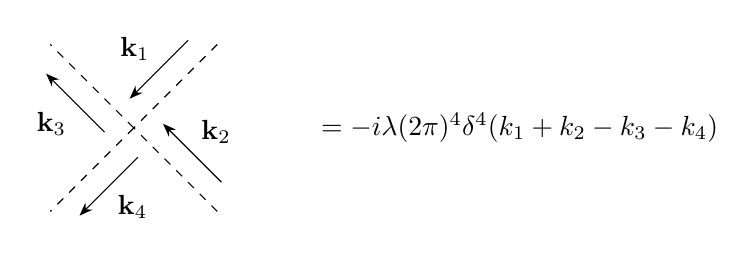
\begin{tikzpicture}[scale=0.7]
            \begin{feynman}
                \vertex (o);
                \vertex [below right =of o] (f2);
                \vertex [below left =of o] (i2);                
                \vertex [above right =of o] (f1);
                \vertex [above left =of o] (i1);
                \diagram*{
                    (f1) -- [scalar, momentum'=$\textbf{k}_1$] (o) --[scalar, momentum=$\textbf{k}_3$] (i1);
                    (f2) -- [scalar, momentum'=$\textbf{k}_2$](o) --[scalar, momentum=$\textbf{k}_4$] (i2);
                };
            \end{feynman}
            \node at (7,0) {\(=-i\lambda(2\pi)^4\delta^4(k_1 + k_2 - k_3 - k_4)\)};
        \end{tikzpicture}
    \end{figure}

    What about the \(\phi\psi\psi^\dagger\) model? Now there are two kinds of particles, and therefore we need to come up with a notation. Let us call the dotted line \(\phi\), line with arrow pointing towards the vertex \(\psi\) and the line with arrow pointing away \(\psi^\dagger\). Therefore, at the vertex, the scalar line meets with a line with arrow pointing towards the vertex and another line with arrow pointing away from the vertex.
    \begin{figure}[h]
        \centering
        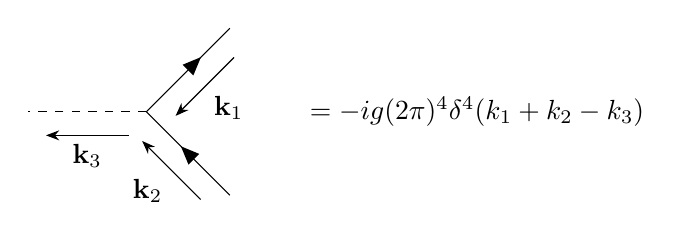
\begin{tikzpicture}[scale=0.7]
            \begin{feynman}
                \vertex (o);
                \vertex [left =of o] (i);                
                \vertex [above right =of o] (f1);
                \vertex [below right =of o] (f2);
                \diagram*{
                    (o) --[scalar, momentum=$\textbf{k}_3$] (i);
                    (f1) -- [anti fermion, momentum=$\textbf{k}_1$] (o);
                    (f2) -- [fermion, momentum=$\textbf{k}_2$] (o);
                };
            \end{feynman}
            \node at (6,0) {\(=-ig(2\pi)^4\delta^4(k_1 + k_2 - k_3)\)};
        \end{tikzpicture}
    \end{figure}
    
    \textcolor{red}{
        Notice that since the in-states enter the calculations as kets and the out-states enter the calculation as bras, the action of \(\psi\) and \(\psi^\dagger\) on the in-states is not the same as their actions on the out-states. That is, if \(\psi\) acts on an in-state it creates an \(N\), while if it acts on an out-state it creates an \(\bar N\), and vice versa for \(\psi^\dagger\). Therefore, the line with arrow towards the vertex, with the momentum also towards the vertex will be an incoming \(N~(\equiv \psi)\) , a line with arrow towards the vertex with momentum arrow away from the vertex will be an outgoing \(\bar N ~(\equiv \psi^\dagger)\), and vice versa for the line whose arrow points away from the vertex.\vspace{7pt}\\
        Therefore the vertex can be interpreted in multiple ways — it can be considered as having one ingoing \(\psi\) and one ingoing \(\bar{\psi}\), or it can be one ingoing \(\psi\) and one outgoing \(\psi\), or it can be one ingoing \(\bar{\psi}\) and one outgoing \(\bar{\psi}\). All these are allowed interpretations of this vertex, and they depend on the momentum flow in the vertex.\\
    }

    The propagators are simply lines connecting two vertices, and they are exactly equal to the value (in momentum space) of the time ordered product of two fields. \\
    That is, for the \(\phi^4\) theory 

    \begin{figure}[h]
        \centering
        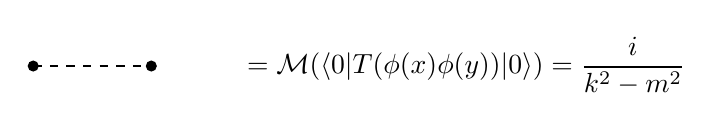
\begin{tikzpicture}
            \begin{feynman}
                \vertex[dot] (a);
                \vertex [dot, right = of a] (b);
                \diagram*{
                    (a) --[scalar] (b);
                };
            \end{feynman};
            \fill (a) circle (2pt);
            \fill (b) circle (2pt);
            \node at (5.5,0) {\(= \mathcal{M}(\braket{0|T(\phi(x)\phi(y))|0}) = \displaystyle \frac{i}{k^2 - m^2}\)};
        \end{tikzpicture}
    \end{figure}

    (where I have used \(\mathcal{M}\) to denote the momentum space representation) and for the \(\psi(\psi^\dagger)\) fields in \(\phi\psi\psi^\dagger\) theory, 
    \begin{figure}[h]
        \centering
        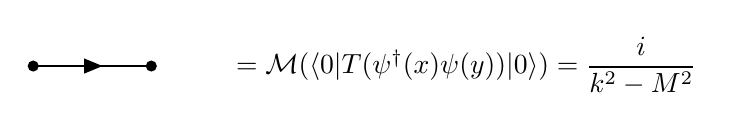
\begin{tikzpicture}
            \begin{feynman}
                \vertex[dot] (a);
                \vertex [dot, right = of a] (b);
                \diagram*{
                    (a) --[fermion] (b);
                };
            \end{feynman};
            \fill (a) circle (2pt);
            \fill (b) circle (2pt);
            \node at (5.5,0) {\(= \mathcal{M}(\braket{0|T(\psi^\dagger(x)\psi(y))|0}) = \displaystyle \frac{i}{k^2 - M^2}\)};
        \end{tikzpicture}
    \end{figure}

    where for the vertex on the left, the line has outgoing arrow and therefore is \(\psi^\dagger\) and for that on the right, the line has incoming arrow and therefore is \(\psi\). Therefore the relevent propagator is \(\braket{0|T(\psi^\dagger(x)\psi(y))|0}\).\\
    
    
    The rules for calculations are simple. You join the vertices with propagators to make a diagram that represents the process you are trying to compute. Label the edges with their corresponding momenta (the momenta decide the flow of the diagram), read off the integrals by assigning the corresponding values, and integrate over all undetermined momenta.\\

    Let us try to get the previously obtained results using these diagrams.\\ The first two are trivial and are directly read from the vertices. The non-trivial result is of the \(NN \to NN\). \\ One possible diagram is 
    \begin{figure}[h]
        \centering
        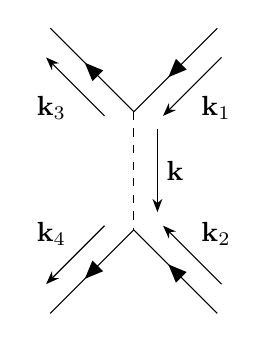
\begin{tikzpicture}
            \begin{feynman}
                \vertex (a);
                \vertex [below = of a] (b);
                \vertex [above left =of a] (f1);                
                \vertex [above right =of a] (i1);
                \vertex [below right =of b] (i2);
                \vertex [below left =of b] (f2);
                \diagram*{
                    (a) --[scalar, momentum=$\textbf{k}$] (b);
                    (i1) -- [fermion, momentum=$\textbf{k}_1$] (a) -- [fermion, momentum=$\textbf{k}_3$] (f1);
                    (i2) -- [fermion, momentum'=$\textbf{k}_2$] (b) -- [fermion, momentum'=$\textbf{k}_4$] (f2);
                };
            \end{feynman}
        \end{tikzpicture}
    \end{figure}

    \textcolor{red}{
        In this diagram the \(\psi\) lines are with in-states and therefore are incoming \(N\) particles, while \(\psi^\dagger\) lines are with out-states and therefore are outgoing \(N\) particles. Therefore this diagram indeed represents a \(NN\to NN\) scattering.\\
    }

    The value of this diagram would be 
    \begin{equation*}
        \int \frac{d^k}{(2\pi)^4}(-ig)(2\pi)^4\delta^4(k_1 - k - k_3)\times(-ig)(2\pi)^4\delta^4(k_2 + k - k_4)\times \frac{i}{k^2 - m^2} 
    \end{equation*}
    which is equal to 
    \begin{equation*}
        -ig^2 (2\pi)^4\delta^4(k_1 +k_2 - k_3 - k_4) \frac{1}{(k_1 - k_3)^2 - m^2}
    \end{equation*}

    There is another diagram that we can draw, since the incoming(outgoing) particles are identical, which is 
    \begin{figure}[h]
        \centering
        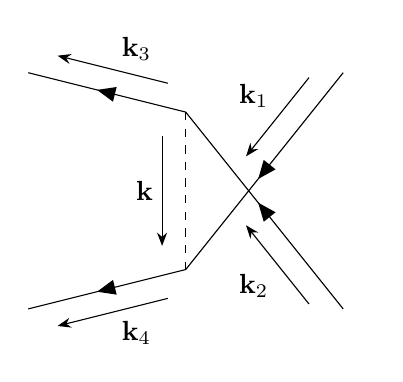
\begin{tikzpicture}
            \begin{feynman}
                % External momenta
                \vertex (i1) at (2,  1.5);
                \vertex (i2) at (2, -1.5);
                \vertex (f1) at ( -2,  1.5);
                \vertex (f2) at ( -2, -1.5);
                % Interaction vertices
                \vertex (a) at (0,  1);
                \vertex (b) at (0, -1);
                % Diagram
                \diagram*{
                (i1) -- [fermion, momentum'={[arrow shorten=0.3,xshift=4mm, yshift=5mm]\(\textbf{k}_1\)}] (b) -- [fermion, momentum=\(\textbf{k}_4\)] (f2),
                (i2) -- [fermion, momentum={[arrow shorten=0.3, ,xshift=4mm, yshift=-5mm]\(\textbf{k}_2\)}] (a) -- [fermion, momentum'=\(\textbf{k}_3\)] (f1),
                (a)  -- [scalar, momentum'=\(\textbf{k}\)] (b),
                };
            \end{feynman}
        \end{tikzpicture}
    \end{figure}

    Notice that the location and direction of the incoming and outgoing momenta should be fixed when we draw different diagrams.\\
    For this diagram, the associated value is 
    \begin{equation*}
        \int \frac{d^k}{(2\pi)^4}(-ig)(2\pi)^4\delta^4(k_1 - k - k_4)\times(-ig)(2\pi)^4\delta^4(k_2 + k - k_3)\times \frac{i}{k^2 - m^2 } 
    \end{equation*}
    which is equal to 
    \begin{equation*}
        -ig^2 (2\pi)^4\delta^4(k_1 +k_2 - k_3 - k_4) \frac{1}{(k_1 - k_4)^2 - m^2}
    \end{equation*}
    And therefore, the amplitude, as before is 
    \begin{equation*}
        -ig^2 (2\pi)^4\delta^4(k_1 +k_2 - k_3 - k_4) \left( \frac{1}{(k_1 - k_3)^2 - m^2 } + \frac{1}{(k_1 - k_4)^2 - m^2 } \right)
    \end{equation*}

    One can attach a \textit{story} to these diagrams, which is to say that two particles approached each other, exchanged a meson and then flew off. This is not to be taken seriously, these diagrams should only be seen as a calculation tool.\\

    Now that we are equipped with the machinery for computing the scattering amplitudes, we can try to calculate the amplitudes for other processes
    
    \subsubsection{Amplitude for \(\bar{N}N\to \bar{N}N\)}
    For this process, we can write the following diagrams 

    \begin{figure}[h]
        \centering
            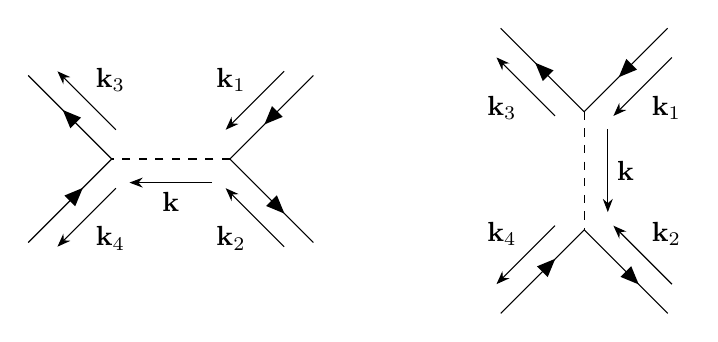
\begin{tikzpicture}
                \begin{feynman}
                    \vertex (a);
                    \vertex [right = of a] (b);
                    \vertex [above left =of a] (f1);                
                    \vertex [above right =of b] (i1);
                    \vertex [below right =of b] (i2);
                    \vertex [below left =of a] (f2);
                    \diagram*{
                        (b) --[scalar, momentum=$\textbf{k}$] (a);
                        (i1) -- [fermion, momentum'=$\textbf{k}_1$] (b);
                        (a) -- [fermion, momentum'=$\textbf{k}_3$] (f1);
                        (i2) -- [anti fermion, momentum=$\textbf{k}_2$] (b);
                        (a) -- [anti fermion, momentum=$\textbf{k}_4$] (f2);
                    };
                \end{feynman}
                \begin{scope}[xshift=6cm, yshift=0.6cm]
                    \begin{feynman}
                        \vertex (a);
                        \vertex [below = of a] (b);
                        \vertex [above left =of a] (f1);                
                        \vertex [above right =of a] (i1);
                        \vertex [below right =of b] (i2);
                        \vertex [below left =of b] (f2);
                        \diagram*{
                            (a) --[scalar, momentum=$\textbf{k}$] (b);
                            (i1) -- [fermion, momentum=$\textbf{k}_1$] (a) -- [fermion, momentum=$\textbf{k}_3$] (f1);
                            (i2) -- [anti fermion, momentum'=$\textbf{k}_2$] (b) -- [anti fermion, momentum'=$\textbf{k}_4$] (f2);
                        };
                    \end{feynman}
                \end{scope}
            \end{tikzpicture}
    \end{figure}

    Notice that we have fixed the statement that the incoming \(N\) has momentum \(\textbf{k}_1\), and \(\bar N\) has momentum \(\textbf{k}_2\) and similarly for outgoing nucleons, and since a nucleon is not the same as an antinucleon, there doesnt exist another diagram as seen in the \(NN\to NN\) process, where the incoming legs are exchanged.\\

    For the first diagram, the value is 
    \begin{equation*}
        \int \frac{d^k}{(2\pi)^4}(-ig)(2\pi)^4\delta^4(k_1 + k_2 - k)\times(-ig)(2\pi)^4\delta^4(k_3 + k_4 - k)\times \frac{i}{k^2 - m^2} 
    \end{equation*}
    which evaluates to 
    \begin{equation*}
        -ig^2(2\pi)^4\delta^4(k_1 + k_2 - k_3 - k_4)\frac{1}{(k_1 + k_2)^2 - m^2 } 
    \end{equation*}
    and the second diagram evaluates to 
    \begin{equation*}
        -ig^2(2\pi)^4\delta^4(k_1 + k_2 - k_3 - k_4)\frac{1}{(k_1 
    - k_3)^2 - m^2} 
    \end{equation*}
    and therefore the total amplitude is 
    \begin{equation*}
        -ig^2(2\pi)^4\delta^4(k_1 + k_2 - k_3 - k_4) \left(  \frac{1}{(k_1 + k_2)^2 - m^2} +    \frac{1}{(k_1 
    - k_3)^2 - m^2}    \right)
    \end{equation*}

    Now the story that goes along these two diagrams are different and not the same as was the case in \(NN\to NN\). The first diagram in this corresponds to the \(N\) and \(\bar{N}\) annihilating each other to give a virtual meson, which then decays back into \(N\bar{N}\) pair. Notice that is a virtual meson and not a real meson since it is not on-shell, i.e., it doesnt have momentum \(k^2 = m^2\), rather its momenta is variable and determined by the incoming particles. The second one corresponds to two particles approach each other, exchange a meson and keep going. 
    
    \subsubsection{Amplitude for \(\phi N \to \phi N\)}
    For this, one possible diagram is 
    \begin{figure}[h]
        \centering
        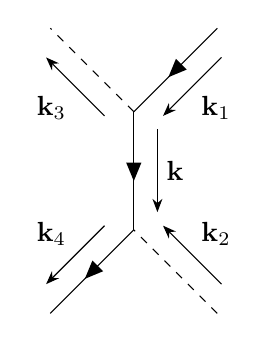
\begin{tikzpicture}
            \begin{feynman}
                \vertex (a);
                \vertex [below = of a] (b);
                \vertex [above left =of a] (f1);                
                \vertex [above right =of a] (i1);
                \vertex [below right =of b] (i2);
                \vertex [below left =of b] (f2);
                \diagram*{
                    (a) --[fermion, momentum=$\textbf{k}$] (b);
                    (i1) -- [fermion, momentum=$\textbf{k}_1$] (a) -- [scalar, momentum=$\textbf{k}_3$] (f1);
                    (i2) -- [scalar, momentum'=$\textbf{k}_2$] (b) -- [fermion, momentum'=$\textbf{k}_4$] (f2);
                };
            \end{feynman}
        \end{tikzpicture}
    \end{figure}
    The value associated with this is 
    \begin{equation*}
        -ig^2 (2\pi)^4\delta^4(k_1 + k_2 - k_3 - k_4) \frac{1}{(k_1- k_3)^2 - M^2}
    \end{equation*}
    The story for this diagram is that a nucleon emits a virtual nucleon and turns into a meson, while the meson absorbs the virtual nucleon and becomes a nucleon. See that with interactions, particle identity is not fixed, particles can convert from one to another. \\
    The other diagram one can draw is 
    \begin{figure}[h]
        \centering
        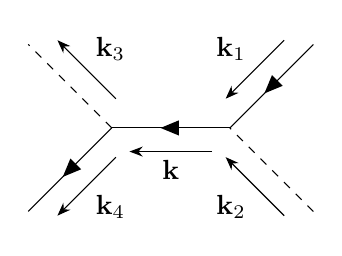
\begin{tikzpicture}
            \begin{feynman}
                    \vertex (a);
                    \vertex [right = of a] (b);
                    \vertex [above left =of a] (f1);                
                    \vertex [above right =of b] (i1);
                    \vertex [below right =of b] (i2);
                    \vertex [below left =of a] (f2);
                    \diagram*{
                        (b) --[fermion, momentum=$\textbf{k}$] (a);
                        (i1) -- [fermion, momentum'=$\textbf{k}_1$] (b);
                        (a) -- [scalar, momentum'=$\textbf{k}_3$] (f1);
                        (i2) -- [scalar, momentum=$\textbf{k}_2$] (b);
                        (a) -- [fermion, momentum=$\textbf{k}_4$] (f2);
                    };
                \end{feynman}
        \end{tikzpicture}
    \end{figure}
    with the associated value 
    \begin{equation*}
        -ig^2 (2\pi)^4\delta^4(k_1 + k_2 - k_3 - k_4) \frac{1}{(k_1+k_2)^2 - M^2}
    \end{equation*}
    The story again is different, the nucleon and meson meet each other and turn into a virtual nucleon which then again emits a nucleon meson pair. The total amplitude, as usual, is the sum of the values for the two diagrams.

    \subsection{Detour — Physics of the Yukawa Potential}
    The Yukawa potential is due to the exchange of massive particles, and is give by 
    \begin{equation*}
        V\sim \frac{e^{-mr}}{r}
    \end{equation*}
    Note that potential is a non-relativistic concept. Relativistic dynamics cannot speak about potential, the reason being the same as discussed int he first section. In case of statics/non-relativistic dynamics, we can speak about potentials, and it is not necessary for all quantum field theories to have deducible potentials. However it is illuminating to see how the things we are calculating in QFT translates to the physics that we can observe. That is, in the non-relativistic limit, the calculations we do in QFT should have some interpretation as some potential.\\

    The objective of this discussion is to consider the process \(NN\to NN\), calculate the \(S-1\) matrix element, find its non-relativistic limit, and then from that, infer what the non-relativistic potential should be. \\
    Remember that for the \(NN\to NN\) process, the matrix element 
    \begin{equation*}
        \bra{\textbf{k}_3, \textbf{k}_4} S-1 \ket{\textbf{k}_1, \textbf{k}_2} = -ig^2 (2\pi)^4\delta^4(k_1 +k_2 - k_3 - k_4) \left( \frac{1}{(k_1 - k_3)^2 - m^2} + \frac{1}{(k_1 - k_4)^2 - m^2 } \right)
    \end{equation*}

    First let us discuss some non-relativistc quantum mechanics. The degrees of freedom are described by a wave function which obeys
    \begin{equation*}
        i\frac{\del}{\del t}\psi(\textbf{x}_1, \textbf{x}_2,t) = \frac{1}{2m}\left( -\mathbf\nabla_1^2 - \mathbf\nabla_2^2 \right) \psi(\textbf{x}_1, \textbf{x}_2,t) + V(\textbf{x}_1 - \textbf{x}_2)\psi(\textbf{x}_1, \textbf{x}_2,t) 
    \end{equation*}
    The potential depends on \(\textbf{x}_1-\textbf{x}_2\) since we require translation invariance in our theory, which was also inherent in our field theoretic description. Since the potential depends only on \(\textbf{x}_1 - \textbf{x}_2\), the simplest kind of wavefunction we can write is of the form
    \begin{equation*}
        \psi = \underbrace{\psi_d(\textbf{x}_1 - \textbf{x}_2, t)}_{\text{wavefunction of separation DOF}}\times \overbrace{\psi_c(\textbf{x}_1 + \textbf{x}_2, t)}^{\text{wavefunction of center of mass DOF}}
    \end{equation*} 
    We can also write the kinetic term in the form 
    \begin{equation*}
        \frac{1}{2m}\left( -\mathbf\nabla_1^2 - \mathbf\nabla_2^2 \right) = \frac{1}{4m}\left( -\mathbf\nabla_{\textbf{x}_1 - \textbf{x}_2}^2 - \mathbf\nabla_{\textbf{x}_1 + \textbf{x}_2}^2 \right)
    \end{equation*}

    \textcolor{red}{
        \begin{equation*}
            \textbf{r} = \textbf{x}_1 - \textbf{x}_2,~~\textbf{R} = \textbf{x}_1 + \textbf{x}_2
        \end{equation*}
        \begin{align*}
            &\mathbf\nabla_1 = \frac{\del \textbf{r}}{\del \textbf{x}_1}\mathbf\nabla_\textbf{r} +  \frac{\del \textbf{R}}{\del \textbf{x}_1}\mathbf\nabla_\textbf{R} = \mathbf{\nabla}_\textbf{r} + \mathbf{\nabla}_\textbf{R}\\
            &\mathbf\nabla_2 = \frac{\del \textbf{r}}{\del \textbf{x}_2}\mathbf\nabla_\textbf{r} +  \frac{\del \textbf{R}}{\del \textbf{x}_2}\mathbf\nabla_\textbf{R} = -\mathbf{\nabla}_\textbf{r} + \mathbf{\nabla}_\textbf{R}
        \end{align*}
        squaring and adding, we get 
        \begin{equation*}
            \mathbf\nabla_1^2 + \mathbf\nabla_2^2 = 2(\mathbf{\nabla}_\textbf{r}^2 + \mathbf{\nabla}_\textbf{R}^2)
        \end{equation*}
    }
    Using this, we can read off the equations of motion for the center of mass and for the separation as 
    \begin{align*}
        &i\frac{\del}{\del t}\psi_c(\textbf{x}_1+ \textbf{x}_2,t) = \frac{1}{4m}\left( -\mathbf\nabla_{\textbf{x}_1 + \textbf{x}_2}^2 \right) \psi_c(\textbf{x}_1 + \textbf{x}_2,t)\\
        &i\frac{\del}{\del t}\psi_d(\textbf{x}_1- \textbf{x}_2,t) = \frac{1}{4m}\left( -\mathbf\nabla_{\textbf{x}_1 - \textbf{x}_2}^2 \right) \psi_d(\textbf{x}_1 - \textbf{x}_2,t) + V(\textbf{x}_1 - \textbf{x}_2)\psi_d(\textbf{x}_1 - \textbf{x}_2,t)
    \end{align*}
    We also want the momentum space representation. Notice that 
    \begin{equation*}
        \exp(i\textbf{k}_1 \cdot \textbf{x}_1 + i\textbf{k}_2 \cdot \textbf{x}_2) = \exp\left( i(\textbf{kx}_1 + \textbf{x}_2)\cdot \frac{(\textbf{k}_1 + \textbf{k}_2)}{2} + i(\textbf{x}_1 - \textbf{x}_2)\cdot \frac{(\textbf{k}_1 - \textbf{k}_2)}{2}     \right)
    \end{equation*}
    What this means is that the momentum associated with the \(\psi_c\) degree of freedom is \((\textbf{k}_1 + \textbf{k}_2)/2\), while \(\psi_d\) has the momentum \((\textbf{k}_1 - \textbf{k}_2)/2\). However, notice that these are not the good momentum eigenstates to expand our position space eigenstates in. This is because the particles are identical and therefore we require the wavefunciton to be symmetric under \(\textbf{x}_1 \leftrightarrow \textbf{x}_2\). \(\psi_c\) already has this property, and on \(\psi_d\) we need to impose this property. Therefore the right eigenstates basis for \(\psi_d\) will not be the complete expontial, but only the cosine part of it. Field theory was clever, it automatically took care of the Bose statistics. But in non-relativistic QM, we need to impose Bose statistics by hand. \\

    We can now calculate the non-relativistic scattering amplitude for this process. The scattering amplitude for \(\psi_c\) and \(\psi_d\) are to be considered separately, and the total amplitude will be the product of these two amplitudes. \\
    First let us consider the COM scattering, which is just free particle scattering. Free particle scattering cannot change the momenta, we need the in momenta to be equal to the out momenta, and therefore the free particle scattering amplitude is simply 
    \begin{equation*}
        (2\pi)^3\delta^3(\textbf{k}_3 +  \textbf{k}_4 - (\textbf{k}_1 + \textbf{k}_2))
    \end{equation*}
    The difference scattering can be calculated using the general non-relativistic scattering amplitude formula 
    \begin{equation*}
        \bra{\textbf{k}'}S-1\ket{\textbf{k}} = -i(2\pi)\delta(E - E') \bra{\textbf{k}} \frac{1}{1 - VG_\perp} -1 \ket{\textbf{k}'}
    \end{equation*}
    To leading order, this is equal to 
    \begin{equation*}
        -i(2\pi)\delta(E - E') \int V(\textbf{x}) \e^{i(\textbf{k} - \textbf{k}')\cdot \textbf{x}}d^3\textbf{x}
    \end{equation*}
    This is for a one particle scattering from a potential. In our case \(\textbf{k} = \textbf{k}_1 - \textbf{k}_2\) and \(\textbf{k}' = \textbf{k}_3 - \textbf{k}_4\). We also need to impose Bose statistics, which means that \(\textbf{k}\to -\textbf{k}\) and \(\textbf{k}' \to -\textbf{k}'\) should also be included, and therefore in our case, the leading order would be 
    \begin{equation*}
        -i(2\pi)\delta(E - E') \int V(\textbf{x}) \left( \e^{i(\textbf{k} - \textbf{k}') \cdot \textbf{x}} + \e^{i(\textbf{k} + \textbf{k}') \cdot \textbf{x}}\right)d^3\textbf{x}
    \end{equation*}
    (where we have not kept track of (a lot of) factors of 2. The important factor is that there will be terms where both initial and final momenta have same sign, and terms where they have the opposite sign.). \\
    
    First take a look at the delta function. The delta function in this term can be expressed in terms of the momenta by seeing that 
    \begin{equation*}
        \delta(E-E') \sim \frac{1}{m}\delta\left((\textbf{k}_1 - \textbf{k}_2)^2 - (\textbf{k}_3 - \textbf{k}_4)^2\right)
    \end{equation*} 
    Now since the total amplitude is the product of this expression with the free particle amplitude, this delta function gets multiplied with \(\delta^3(\textbf{k}_3 +  \textbf{k}_4 - (\textbf{k}_1 + \textbf{k}_2))\), and therefore we can add \((\textbf{k}_1 + \textbf{k}_2)^2\)   and subtract \((\textbf{k}_3 + \textbf{k}_4)^2\) to get 
    \begin{equation*}
        \delta(E-E') \sim \frac{1}{m}\delta\left((\textbf{k}_1 - \textbf{k}_2)^2 + (\textbf{k}_1 + \textbf{k}_2)^2 - (\textbf{k}_3 - \textbf{k}_4)^2 - (\textbf{k}_3 + \textbf{k}_4)^2\right) = \sim \frac{1}{m}\delta(k_1^2 + k_2^2 - k_3^2 - k_4^2)
    \end{equation*}
    This is the non relativistic limit of the delta function 
    \begin{equation*}
        \delta(k_1^0 + k_2^0 - k_3^0 - k_4^0)
    \end{equation*}
    and therefore 
    \begin{equation*}
         (2\pi)^4\delta(E-E')\delta^3(\textbf{k}_3 +  \textbf{k}_4 - (\textbf{k}_1 + \textbf{k}_2))\overset{\text{non-relativistic}}{=}(2\pi)^4\delta^4(k_1 + k_2 - k_3 - k_4) 
    \end{equation*}

    In the amplitude we calculated from the field theory, the delta function was multiplied by terms of the form \(((k_1 - k_3)^2 - m^2)^{-1}\), which are four vector terms. We need to match these terms too in our non-relativistic calculations. To do so, we can make use of the fact that the field theoretic amplitude is Lorentz invariant, and therefore we can choose to go to the COM frame. In the COM frame, we have \(\textbf{k}_1 = -\textbf{k}_2\) and \(\textbf{k}_3 = -\textbf{k}_4\), which means that the energies are the same, i.e. \(k_1^0 = k_2^0 = k_3^0 = k_4^0\). Therefore, the term
    \begin{equation*}
        -ig^2\left( \frac{1}{(k_2 - k_4)^2 - m^2} + \frac{1}{(k_1 - k_4)^2 - m^2 } \right) = ig^2\left( \frac{1}{(\textbf{k}_2 - \textbf{k}_4)^2 + m^2} + \frac{1}{(\textbf{k}_1 - \textbf{k}_4)^2 + m^2 } \right)
    \end{equation*}

    In the COM frame, \(\textbf{k}' = \textbf{k}_3 - \textbf{k}_4 = 2\textbf{k}_3 = -2\textbf{k}_4\) and \(\textbf{k} = \textbf{k}_1 - \textbf{k}_2 = 2\textbf{k}_1 = -2\textbf{k}_2\). Therefore 
    \begin{equation*}
        \textbf{k} - \textbf{k}' \sim \textbf{k}_2 -  \textbf{k}_4
    \end{equation*}
    and  
    \begin{equation*}
        \textbf{k} + \textbf{k}' \sim \textbf{k}_1 -  \textbf{k}_4
    \end{equation*}

    which means the above term would be 
    \begin{equation}
        ig^2\left( \frac{1}{(\textbf{k} - \textbf{k}')^2 + m^2} + \frac{1}{(\textbf{k} + \textbf{k}')^2 + m^2 } \right)
    \end{equation}
    \textit{in COM frame only}.\\

    Therefore, we need a potential \(V(r)\) such that 
    \begin{equation*}
        \int V(\textbf{x}) \left( \e^{i(\textbf{k} - \textbf{k}') \cdot \textbf{x}} + \e^{i(\textbf{k} + \textbf{k}') \cdot \textbf{x}}\right)d^3\textbf{x} \sim \left( \frac{1}{(\textbf{k} - \textbf{k}')^2 + m^2} + \frac{1}{(\textbf{k} + \textbf{k}')^2 + m^2 } \right)
        \label{eq:yukawa-potential-calc}
    \end{equation*}

    The general integral 
    \begin{equation*}
        \int V(\textbf{x})\e^{i\textbf{q}\cdot \textbf{x}}d^3\textbf{x}
    \end{equation*}
    can be calculated by going to polar coordinates (assuming the potential to be spherically symmetric) as
    \begin{equation*}
        2\pi \int V(r) \e^{iqr\cos\theta} d(\cos\theta)r^2dr = 4\pi \int V(r)\frac{r}{q} \sin(qr) dr
    \end{equation*}
    Therefore, for the equation (\ref{eq:yukawa-potential-calc}) to be true, we require
    \begin{equation*}
        \int V(r)\frac{r}{q} \sin(qr) dr = \frac{1}{q^2 + m^2}
    \end{equation*}

    Now we have 
    \begin{equation*}
        \int \frac{\e^{-mr}}{r}\frac{r\sin(qr)}{q} dr = \mathrm{Im}\int \frac{\e^{-mr+iqr}}{q} dr = \mathrm{Im}\left(\frac{1}{q}\frac{m+iq}{m^2 + q^2}\right) = \frac{1}{q^2 + m^2}
    \end{equation*}
    and therefore we get 
    \begin{equation*}
        V(r) \sim \frac{\e^{-mr}}{r}
    \end{equation*}

    \subsection{Crossing Symmetry in Feynman Diagrams}
    It refers to the fact that the amplitudes for some processes are related to the amplitudes for some other processes where some of the incoming and outgoing momenta are exchanged. That is, it is the statement that sometimes we can make various transformations to Feynman Diagrams and obtain different processes with same amplitude. The simplest example is the previously studied vertex 
    \begin{figure}[h]
        \centering
        \begin{tikzpicture}[scale=0.8]
            \begin{feynman}
                \vertex (a);
                \vertex[above right=of a] (b);
                \vertex[below right=of a] (c);
                \vertex[left = of a] (d);
                \diagram*{
                    (d) -- [scalar] (a) -- [anti fermion] (b);
                    (a) -- [fermion] (c);
                };
            \end{feynman}
        \end{tikzpicture}
    \end{figure}
    There are six possible physical interpretations of this vertex, corresponding to \(2^3 - 2\) possible momentum directions (subtract 2 since all momenta inwards and all momenta outwards make no sense physically)
    \begin{enumerate}
        \item Nucleon and anti nucleon annihilate to give meson \begin{figure}[h]
        \centering
        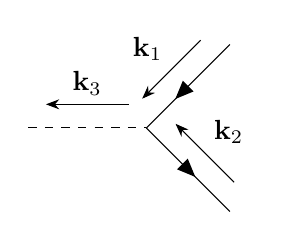
\begin{tikzpicture}[scale=0.8]
            \begin{feynman}
                \vertex (a);
                \vertex[above right=of a] (b);
                \vertex[below right=of a] (c);
                \vertex[left = of a] (d);
                \diagram*{
                    (d) -- [scalar, rmomentum=\(\textbf{k}_3\)] (a) -- [anti fermion, rmomentum=\(\textbf{k}_1\)] (b);
                    (a) -- [fermion, rmomentum=\(\textbf{k}_2\)] (c);
                };
            \end{feynman}
        \end{tikzpicture}
    \end{figure}
    \item Meson creates a nucleon - anti nucleon pair \begin{figure}[h]
        \centering
        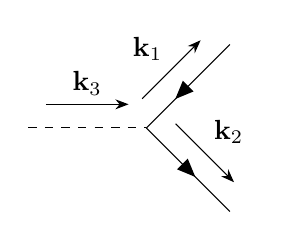
\begin{tikzpicture}[scale=0.8]
            \begin{feynman}
                \vertex (a);
                \vertex[above right=of a] (b);
                \vertex[below right=of a] (c);
                \vertex[left = of a] (d);
                \diagram*{
                    (d) -- [scalar, momentum=\(\textbf{k}_3\)] (a) -- [anti fermion, momentum=\(\textbf{k}_1\)] (b);
                    (a) -- [fermion, momentum=\(\textbf{k}_2\)] (c);
                };
            \end{feynman}
        \end{tikzpicture}
    \end{figure}
    \item Anti-nucleon emits a meson and continues as an anti-nucleon \begin{figure}[h]
        \centering
        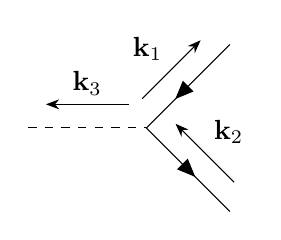
\begin{tikzpicture}[scale=0.8]
            \begin{feynman}
                \vertex (a);
                \vertex[above right=of a] (b);
                \vertex[below right=of a] (c);
                \vertex[left = of a] (d);
                \diagram*{
                    (d) -- [scalar, rmomentum=\(\textbf{k}_3\)] (a) -- [anti fermion, momentum=\(\textbf{k}_1\)] (b);
                    (a) -- [fermion, rmomentum=\(\textbf{k}_2\)] (c);
                };
            \end{feynman}
        \end{tikzpicture}
    \end{figure}
    \item Nucleon emits a meson and continues as a nucleon \begin{figure}[h]
        \centering
        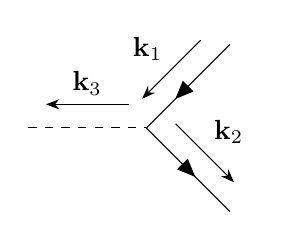
\begin{tikzpicture}[scale=0.8]
            \begin{feynman}
                \vertex (a);
                \vertex[above right=of a] (b);
                \vertex[below right=of a] (c);
                \vertex[left = of a] (d);
                \diagram*{
                    (d) -- [scalar, rmomentum=\(\textbf{k}_3\)] (a) -- [anti fermion, rmomentum=\(\textbf{k}_1\)] (b);
                    (a) -- [fermion, momentum=\(\textbf{k}_2\)] (c);
                };
            \end{feynman}
        \end{tikzpicture}
    \end{figure}
    \item Anti-nucleon absorbs a meson and continues as an anti-nucleon \begin{figure}[H]
        \centering
        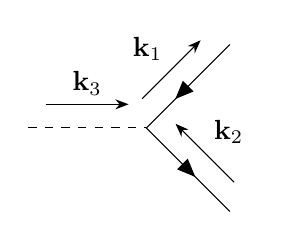
\begin{tikzpicture}[scale=0.8]
            \begin{feynman}
                \vertex (a);
                \vertex[above right=of a] (b);
                \vertex[below right=of a] (c);
                \vertex[left = of a] (d);
                \diagram*{
                    (d) -- [scalar, momentum=\(\textbf{k}_3\)] (a) -- [anti fermion, momentum=\(\textbf{k}_1\)] (b);
                    (a) -- [fermion, rmomentum=\(\textbf{k}_2\)] (c);
                };
            \end{feynman}
        \end{tikzpicture}
    \end{figure}
    \item Nucleon absorbs a meson and continues as a nucleon \begin{figure}[H]
        \centering
        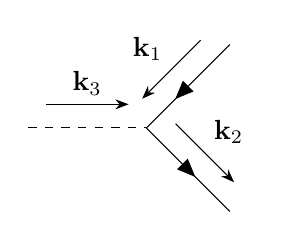
\begin{tikzpicture}[scale=0.8]
            \begin{feynman}
                \vertex (a);
                \vertex[above right=of a] (b);
                \vertex[below right=of a] (c);
                \vertex[left = of a] (d);
                \diagram*{
                    (d) -- [scalar, momentum=\(\textbf{k}_3\)] (a) -- [anti fermion, rmomentum=\(\textbf{k}_1\)] (b);
                    (a) -- [fermion, momentum=\(\textbf{k}_2\)] (c);
                };
            \end{feynman}
        \end{tikzpicture}
    \end{figure}
    \end{enumerate}
    The Feynman diagrams for all these diagrams always assign to these diagrams a \(-ig\). The only difference is the signs of the momenta entering the delta function. Its redundent to think of these processes differently, and therefore one can write a compact notation to represent all these values in a single diagram. The notation is to mark all the external momenta as incoming. This is fine since all the external momenta have a particular property, that is, they are on shell \(k_i^2 = m^2/M^2\) and they have positive Energy, i.e.\ \(k_i^0 > 0\). Therefore, when we mark all the momenta as incoming, the actual outgoing momenta will have \(k_i^0<0~\because k_i^\mu = -p^\mu\) for outgoing, and therefore \(k_i^0 = -p^0 < 0\) . And this will mean that the physical particle is outgoing. Therefore, it is consistent to mark all momenta as incoming since the outgoing particles will automatically get assigned a negative energy, therefore removing confusion. Therefore, we can denote all these scattering amplitudes by 
    \begin{equation*}
        -ig(2\pi)^4\delta^4(k_1 + k_2 + k_3)
    \end{equation*}

    This can be extended to more complicated diagrams too. As an example, the diagram 
    \begin{figure}[H]
        \centering
        \begin{tikzpicture}[scale=0.8]
            \begin{feynman}
                \vertex (a);
                \vertex[above right=of a] (i1) {\(\textbf{k}_1\)};
                \vertex[below right=of a] (i2) {\(\textbf{k}_2\)};
                \vertex[above left=of d] (f1) {\(\textbf{k}_3\)};
                \vertex[below left=of d] (f2) {\(\textbf{k}_4\)};
                \vertex[left = of a] (b);
                \diagram*{
                    (d) -- [scalar] (a) -- [anti fermion] (i1);
                    (a) -- [fermion] (i2);
                    (d) -- [fermion] (f1);
                    (d) -- [fermion] (f2);
                };
            \end{feynman}
            \node at (6.5,0) {\(=\displaystyle -ig^2\frac{1}{(k_1+k_2)^2 - m^2}(2\pi)^4\delta^4(k_1+k_2+k_3+k_4)\)};
        \end{tikzpicture}
    \end{figure}
    There is another different diagram we need to consider, owing to Bose statistics, which is the following
    \begin{figure}[H]
        \centering
        \begin{tikzpicture}[scale=0.8]
            \begin{feynman}
                \vertex (a);
                \vertex[above right=of a] (i1) {\(\textbf{k}_1\)};
                \vertex[below right=of a] (i2) {\(\textbf{k}_2\)};
                \vertex[above left=of d] (f1) {\(\textbf{k}_3\)};
                \vertex[below left=of d] (f2) {\(\textbf{k}_4\)};
                \vertex[left = of a] (b);
                \diagram*{
                    (d) -- [scalar] (a) -- [anti fermion] (i2);
                    (d) -- [fermion] (i1);
                    (a) -- [fermion] (f1);
                    (d) -- [anti fermion] (f2);
                };
            \end{feynman}
            \node at (6.5,0) {\(=\displaystyle -ig^2\frac{1}{(k_1+k_3)^2 - m^2}(2\pi)^4\delta^4(k_1+k_2+k_3+k_4)\)};
        \end{tikzpicture}
    \end{figure}
    and the full amplitude is the sum of these two diagrams. What crossing symmetry says is that these are the only possible diagrams, and one can read off all possible processes from this by choosing which \(k_i^0\) to set negative.\\

    To look at it in action, consider the original old diagrams for \(N\bar{N} \to N \bar N\).
    \begin{figure}[h]
        \centering
            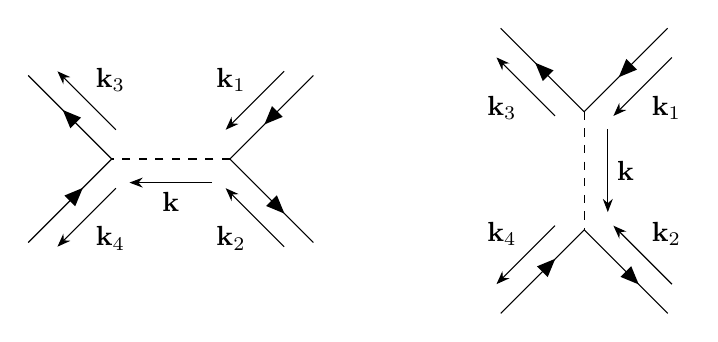
\begin{tikzpicture}
                \begin{feynman}
                    \vertex (a);
                    \vertex [right = of a] (b);
                    \vertex [above left =of a] (f1);                
                    \vertex [above right =of b] (i1);
                    \vertex [below right =of b] (i2);
                    \vertex [below left =of a] (f2);
                    \diagram*{
                        (b) --[scalar, momentum=$\textbf{k}$] (a);
                        (i1) -- [fermion, momentum'=$\textbf{k}_1$] (b);
                        (a) -- [fermion, momentum'=$\textbf{k}_3$] (f1);
                        (i2) -- [anti fermion, momentum=$\textbf{k}_2$] (b);
                        (a) -- [anti fermion, momentum=$\textbf{k}_4$] (f2);
                    };
                \end{feynman}
                \begin{scope}[xshift=6cm, yshift=0.6cm]
                    \begin{feynman}
                        \vertex (a);
                        \vertex [below = of a] (b);
                        \vertex [above left =of a] (f1);                
                        \vertex [above right =of a] (i1);
                        \vertex [below right =of b] (i2);
                        \vertex [below left =of b] (f2);
                        \diagram*{
                            (a) --[scalar, momentum=$\textbf{k}$] (b);
                            (i1) -- [fermion, momentum=$\textbf{k}_1$] (a) -- [fermion, momentum=$\textbf{k}_3$] (f1);
                            (i2) -- [anti fermion, momentum'=$\textbf{k}_2$] (b) -- [anti fermion, momentum'=$\textbf{k}_4$] (f2);
                        };
                    \end{feynman}
                \end{scope}
            \end{tikzpicture}
    \end{figure}
    which had the amplitude as
    \begin{equation*}
        -ig^2(2\pi)^4\delta^4(k_1 + k_2 - k_3 - k_4) \left(  \frac{1}{(k_1 + k_2)^2 - m^2} +    \frac{1}{(k_1 
    - k_3)^2 - m^2}    \right)
    \end{equation*}
    This can be exactly obtained by the above two digrams in our new conventions, by doing \(k_{3/4} = -k_{3/4}\). Notice that in the new convention, we justified the second diagram by invoking Bose statistice, but in the original diagrams, we said that the Bose statistics was not really important. This is due to the fact that the processess \(N\bar{N}\to N\bar N\),  \(\bar N\bar{N}\to \bar N\bar N\), \(NN\to NN\), etc., are all related to one another by this crossing symmetry, and if Bose statistics is invoked in one, it can and should be invoked in some way in all other.\\

    Let us look at another process \(N\bar N \to \phi\phi\)
    \begin{figure}[h]
        \centering
            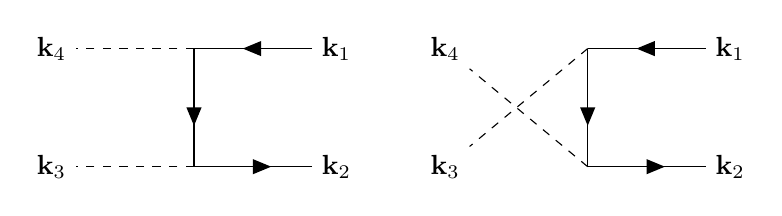
\begin{tikzpicture}
                \begin{feynman}
                    \vertex (a);
                    \vertex [below = of a] (b);
                    \vertex [left =of a] (f1) {\(\textbf{k}_4\)};                
                    \vertex [right =of a] (i1) {\(\textbf{k}_1\)};
                    \vertex [right =of b] (i2) {\(\textbf{k}_2\)};
                    \vertex [left =of b] (f2) {\(\textbf{k}_3\)};
                    \diagram*{
                        (b) --[anti fermion] (a);
                        (i1) -- [fermion] (a);
                        (a) -- [scalar] (f1);
                        (i2) -- [anti fermion] (b);
                        (b) -- [scalar] (f2);
                    };
                \end{feynman}
                \begin{scope}[xshift=5cm]
                        \begin{feynman}
                        \vertex (a);
                        \vertex [below = of a] (b);
                        \vertex [left =of a] (f1) {\(\textbf{k}_4\)};                
                        \vertex [right =of a] (i1) {\(\textbf{k}_1\)};
                        \vertex [right =of b] (i2) {\(\textbf{k}_2\)};
                        \vertex [left =of b] (f2) {\(\textbf{k}_3\)};
                        \diagram*{
                            (b) --[anti fermion] (a);
                            (i1) -- [fermion] (a);
                            (a) -- [scalar] (f2);
                            (i2) -- [anti fermion] (b);
                            (b) -- [scalar] (f1);
                        };
                    \end{feynman}
                \end{scope}
            \end{tikzpicture}
    \end{figure}

    In the new convention, with all momenta incoming, these two are the only possible diagrams, and they give the total amplitude 
    \begin{equation*}
        -ig^2(2\pi)^4\delta^4(k_1+k_2+k_3+k_4) \left(  \frac{1}{(k_1+k_4)^2 - m^2} + \frac{1}{(k_1+k_3)^2 - m^2}  \right)
    \end{equation*}

    Now using the same diagram, we can represent also the processes \(N+\phi \to N + \phi\), \(\phi\phi\to N N\), \(\phi\phi\to \bar N \bar N\) etc.

    \subsection{Mandelstam Variables}
    Notice that in the 4 point processes that we have calculated so far, we have always encountered terms like \((k_1 + k_3)^2\), \((k_1 + k_4)^2\), etc. We can define a different kinematic representation for momenta that are slightly more convenient in representing the above combinations. These are called Mandelstam variables.\\

    Suppose the four momenta are \(k_1,~k_2,~k_3,~k_4\) (all incoming), then 
    \begin{enumerate}
        \item \(s = (k_1 + k_2)^2\)
        \item \(t = (k_1 + k_3)^2\)
        \item \(u = (k_1 + k_4)^2\)
    \end{enumerate}

    These are all Lorentz invariant, and they are basically the only unique Lorentz invariant we can construct out of the incoming momenta. All other Lorentz invariant objects (like \(k_1\cdot k_2\) etc) can be written in terms of these. Therefore, all the amplitudes we write should be only functions of \(s,~t,~\& ~u\). However these are not all independent, they satisfy 
    \begin{align*}
        2(s+t+u) &= (k_1 + k_2)^2 + (k_1 + k_3)^2 + (k_1 + k_4)^2\\
            &=(k_3 + k_4)^2 + (k_2 + k_4)^2 + (k_2 + k_3)^2~~(\because k_1 + k_2 + k_3 + k_4 = 0)\\
            &= 3(k_1^2 + k_2^2 + k_3^2 + k_4^2 ) + 2k_1\cdot k_2 + \text{~other combinations}
    \end{align*}
    Note that \((k_1 + k_2 + k_3 + k_4)^2  = 0 = k_1^2 +\cdot+2k_1 \cdot k_2 + \cdot \) . Therefore, we get 
    \begin{align*}
        &2(s+t+u) = 2(k_1^2 + k_2^2 + k_3^2 + k_4^2) + 0 = 2(\sum_i m_i^2)\\
        \implies & s+t+u = \sum m_i^2
    \end{align*}
    Therefore in the above \(N\bar N \to \phi\phi\), the two diagrams have propagators in \(t\) and \(u\), and they are called \(t-\)channel and \(u-\)channel diagrams.\\

    The Mandelstam variables are useful even in higher point scatterings, however they become a little complicated sometimes. For higher point correlators, the definitions of Mandelstam variables are also standardized. That is, 
    \begin{equation*}
        s_{ij} = k_i\cdot k_j
    \end{equation*}
    But for these, we get more constraints beyond the obvious constraints we got from \(\sum k_i = 0\) and \(k_i^2 = m_i^2\). To see how, lets drop \(s_{nj}\) (where \(n\) is the number of incoming momenta), since \(k_n = -\sum_{i=1}^{n-1}k_i\). We are left with 
    \begin{equation*}
        {}^{n-1}C_2 = \frac{(n-1)(n-2)}{2}
    \end{equation*}
    variables since we can choose \(i\) in \(n-1\) ways (leaving \(n\)) and \(j\) in \(n-2\) ways. That is, we drop all \(s_{nj}\)s since we can write the \(s_{nj}\) in terms of \(k_i,~i\ne n\), and \(s_{ij} = s_{ji}\). Therefore we need to choose \(i\) from \(n-1\) numbers and \(j\) from \(n-2\) numbers. \\

    Now in \(d\) dimensions, for \(n\) point scattering, there are \(n(d-1)\) degrees of freedom (\(d-1\) and not \(d\) because of mass shell condition). Then there are additional \(d\) delta function constraints for the momenta, and therefore the total degrees of freedom is 
    \begin{equation*}
        d(n-1) - d
    \end{equation*}

    Notice that we have now \(\propto n\) degrees of freedom, and \(\propto n^2\) free Mandelstam variables, and therefore, there are more constraints, which are not trivial but are some non-trivial non-linear constraints, that should bring down the variables to \(\propto n\). This is something we need to keep in mind when working with scattering amplitudes. One way to get around this is to consider scattering in large dimensions, say \(n\), in some processes where the details of the scattering doesn't depend on the dimensionality of the space. Then one can use Mandelstam variables, and calculate the kinematics. But we need to remember that, in finite dimensions, for higher point processes, there are some more constraints that exist, but it is very difficult to handle these, in-fact there is no existing method to obtain the constraints given an \(n-\)point scattering in \(d\) dimensions. Often, it is fine to treat the Mandelstam variables as independent, since the additional non-linear constraint do not have much affect on the kinematics.

    \subsection{Probabilities and Cross-Sections}

    What we calculated so far was amplitudes. To get probabilities we should simply square them. The amplitudes are always of the form 
    \begin{equation*}
        M_{\text{if}}~ (2\pi)^4\delta^4(k_i - k_f)
    \end{equation*}
    and squaring this to get the probability requires us to ``square'' the delta function, which makes no sense mathematically.\\
    
    Conceptually speaking, this problem arises because we chose our in and out states as plane wave states, which are not normalisable. If instead we had chosen to work with smeared in and out states normalised to \(1\), the delta functions would pair with the integration associated with the smearing, and give a finite number for the probability. Notice that the valid physical object is the smeared state, and it is this smeared state that one encounters in experiments. Therefore, we should be studying the wavepackets, which would be a physically right kind of state, and would also circumvent the problem of squaring the delta function.\\

    In practice, we never do this. If we introduce wavepacket in-out states, the results will depend on the form of the wavepackets we consider, and therefore some arbitrariness will creep into our results and we loose the universality of the results we obtain. Further, when we do experiments, the particles we encounter are almost of the form of plane waves with a little spread (i.e.\ they have a spread very large compared to the region of interaction, and also have sharp momentum distributions), but to an approximation one can always drop this spread and say that the particle has a fixed momentum \(k\). Therefore, if we ask the \textit{physically right kind of questions}, we can continue to work with plane wave approximations. \\
    
    To be precise, in the following section, we will regulate our calculations by considering wavepackets, and in the end we will consider some limits where the details of the wavepackets do not matter. \\

    The first point is, there are two kinds of plane waves, the incoming plane waves and the outgoing plane waves. At the level of amplitude, there was a symmetry in how the incoming and outgoing states were treated. But when we discuss probabilities, there arises an asymmetry in how we treat them. That is, when discussing probabilities, we average over the initial states and sum over the final states. This is the kind of question we choose to ask. Mathematically, we could have chosen a different question, but this is a physically relevant question. Physically, we are setting up an experiment and there is an uncertainity in the initial conditions due to verious experimental errors, and therefore we average over the initial states, and then there are various possible outcomes and we sum over them. \textcolor{red}{(That is, if we have a few mutually exclusive possible outcomes, the total probability is the sum of the probabilities for the individual processes. As an example consider a process where two electrons are produced. There are different possible outcomes regarding the different possible spins. The probability for the production of two electrons would be the sum of the probabilities of electron production with different spin combinations. This is the right kind of question to ask physically.)}\\

    What this means in our case of scattering is that, we consider an initial state of the form \\
    \(\ket{\text{in}} = \int \psi(p_i) \ket{p_1, \ldots, p_n}\), with \(\braket{\text{in}|\text{in}} = \int \psi(p_i)^2 dp_i = 1\), and ask for the the probability to scatter into \(k_f^i + dk_f^i\) for every final state \(k_f^i\). The wavepacket in-state has an integral over the momenta, and therefore absorbs the delta function in the amplitude, giving a finite value. Therefore, we do not need to consider wavepackets in the final states, but just ask for a probability to scatter into an infinitesimal spread in the momenta. \\ 
    That is, the probability we will consider will be 
    \begin{equation*}
        dP = |\braket{\text{in}~| ~k_1, \ldots, k_m}|^2 \frac{d^3\textbf{k}_1}{(2\pi)^3 2\w_\mathbf{k_1}}\cdots \frac{d^3\textbf{k}_m}{(2\pi)^3 2\w_\mathbf{k_m}}
    \end{equation*}
    Note that \(\braket{\text{in}~| ~k_1, \ldots, k_m}\) is already finite. Also note that if \(\psi(p_i)\) was a delta function in the \(p_i\)s then the delta function in the amplitude would survive and we would not get a finite answer. For the general case when \(\ket{\text{in}}\) is not necessarily normalised, the infinitesimal probability would be 
    \begin{equation*}
        dP = \frac{|\braket{\text{in}~| ~k_1, \ldots, k_m}|^2}{\braket{\text{in}|\text{in}}}\frac{d^3\textbf{k}_1}{(2\pi)^3 2\w_\mathbf{k_1}}\cdots \frac{d^3\textbf{k}_m}{(2\pi)^3 2\w_\mathbf{k_m}}
    \end{equation*}
    
    Although the value is finite now, we still have an arbitrariness in the probability since there is a wavepacket in the in-state. We want to get rid of this, by considering in-states that are very close to plane waves. That is, we study the limit where the in-states are plane waves. One way to take this limit is by making the plane wave states normalisable by putting the in-states in a box. That is, we take a box of side \(L\), and consider that all processess happen within this box in a time interval \(T\). In this box, the plane waves are normalisable, and in the limit \(L,T\to\infty\) we recover the original plane waves. \\

    When we go back to plane wave incoming states, the delta functions reappear. But see that the problematic term in the amplitude squared was 
    \begin{equation*}
        \left((2\pi)^4 \delta^4(\sum k_i + \sum p_i)\right)^2 
    \end{equation*}
    where the delta functions came from 
    \begin{equation*}
        \left((2\pi)^4 \delta^4(\sum k_i + \sum p_i)\right)^2 = \left((2\pi)^4 \delta^4(Q)\right)^2\sim  \lim_{L,T\to \infty}\int \e^{iQ\cdot x} d^4x \int \e^{iQ\cdot y}d^4y
    \end{equation*}
    We do a bit of handwavery here, you can do the calculations precisely by taking a plane wave limit of the wavepacket and somehow turning off interactions in far past and see that the calculations do match, but here we do not keep that level of precision. \\
    Notice that in doing the first integral above, we get a delta function, which we can use to set \(Q=0\) in the second integrand, giving
    \begin{equation*}
        \left((2\pi)^4 \delta^4(Q)\right)^2\sim  \lim_{L,T\to \infty}(2\pi)^4 \delta^4(Q) \int 1~d^4y = \lim_{V,T\to \infty}VT (2\pi)^4 \delta^4(Q) 
    \end{equation*}
    (where \(V=L^3\)) is the volume of the space.\\
    Further, in the plane wave limit, the denominator \(\braket{\text{in}|\text{in}}\) is no longer \(1\), but becomes 
    \begin{equation*}
        (2\pi)^3\delta(0)2\w_\textbf{p}
    \end{equation*}
    which happens because of our normalisation 
    \begin{equation*}
        \braket{\textbf{p}|\textbf{p}'} = (2\pi)^3 \delta^3(\textbf{p} - \textbf{p}')2\w_\textbf{p}
    \end{equation*}
    But this delta function also arises due to an integral over spacetime as 
    \begin{equation*}
        \braket{\textbf{p}|\textbf{p}'} = (2\pi)^3 \delta^3(\textbf{p} - \textbf{p}')2\w_\textbf{p} = 2\sqrt{\w_\textbf{p}\w_\textbf{p'}}\lim_{L,T\to\infty} \int \e^{-i(\textbf{p}-\textbf{p}')\cdot \textbf{x}} d^3\textbf{x}
    \end{equation*}
    which in \(\textbf{p}=\textbf{p}'\) case, gives 
    \begin{equation*}
        \braket{\text{in}|\text{in}} = 2\w_\textbf{p}\lim_{L,T\to\infty} \int 1~d^3\textbf{x} = 2\w_\textbf{p}\lim_{V,T\to\infty} V
    \end{equation*}
    For \(n\) incoming particles, this would be 
    \begin{equation*}
        \braket{\textbf{p}_1,\ldots,\textbf{p}_n|\textbf{p}_1,\ldots,\textbf{p}_n} = \lim_{V,T\to\infty} V^n \prod_{i} (2\w_\mathbf{p_i})
    \end{equation*}

    Putting all these together, we get 
    \begin{equation*}
        dP = |M_{\text{if}}|^2 \left(\prod_{j\in\text{out}}\frac{d^3\textbf{k}_j}{(2\pi)^3 2E_j}\right) \left(\prod_{i\in \text{in}} \frac{1}{2E_i}   \right)\times (2\pi)^4\delta^4\left(\sum k_{\text{in}} - \sum k_{\text{out}} \right)\lim_{V,T\to \infty}\frac{VT}{V^n}
    \end{equation*}
    where \(M_{\text{if}}\) is the part of the amplitude that doesn't contain the delta function. Notice that this experession still has the regulators in the form of volume and time factors.\\

    Now, if we ask the \textit{right kind of physical questions}, the volume and time factors and limits will become irrelevant. Let us consider a few cases. To see what are the questions we should ask, consider first the decay of a particle, which has \(n=1\). In this case, the volume factors cancel off immediately, and only the T factor remains. Therefore the physical question to ask is the \textbf{decay probability per unit time}, which is given by 

    \begin{equation*}
        \overbrace{\frac{1}{2E_{\text{in}}}}^{\text{not L.I}} \underbrace{| M_{\text{if}}|^2 \left(\prod_{j\in\text{out}}\frac{d^3\textbf{k}_j}{(2\pi)^3 2E_j}\right) \times (2\pi)^4\delta^4\left(\sum k_{\text{in}} - \sum k_{\text{out}} \right)}_{L.I}
    \end{equation*}
    where we see that the answer is not Lorentz Invariant (L.I), since the decay probability per unit \textit{time} depends on which frame we are in. The decay probability is minimized in the incoming particle's rest frame, where \(E_{\text{in}} = m\). The decay lifetime, which is the inverse of the decay probability per unit time, therefore satisfies
    \begin{equation*}
        \frac{t^{\text{life}}_{\text{moving}}}{t^{\text{life}}_{\text{rest}}} = \frac{E_{\text{moving}}}{m}
    \end{equation*}
    That is, sometimes a particle that is very short lived can have a longer lifetime by boosting the particle. This is a standard example we consider when we learn special relativity — the muon decay.

    Let us consider the case \(n=2\). In this case, the right question to ask would be the \textit{differential cross-section} which is the \textbf{probability per unit time per unit of incoming flux}. This is what is is measured in an experiment, and also gives a finite and right answer when calculated. \\
    
    To discuss this, we first need to do a kinematic computation of flux. Suppose there is a volume \(V = L^3\), with one particle having velocity \(\textbf{v}\) at an instant. What we want is the flux of this particle as it goes by. Flux is given by number of particles per unit area per time. In this case, the number of particles is \(1\), the area of a side is \(L^2\) and the time taken for the particle to cross the volume is \(\displaystyle\frac{L_1}{v}\). Therefore, the flux is 
    \begin{equation*}
        \text{flux} = \frac{|\textbf{v}|}{L}\frac{1}{L^2} = \frac{|\textbf{v}|}{L^3} = \frac{|\textbf{v}|}{V}
    \end{equation*}
    What we have is two particles approaching each other, in which case the flux would be 
    \begin{equation*}
        \text{flux} = \frac{|\textbf{v}_1 - \textbf{v}_2|}{V}
    \end{equation*}

    The differential cross section is given by 
    \begin{equation*}
        d\sigma = \lim_{V,T\to \infty} |M_{\text{if}}|^2 \left(\frac{1}{2E_1}\frac{1}{2E_2} \right)\left(\prod_{j\in\text{out}}\frac{d^3\textbf{k}_j}{(2\pi)^3 2E_j}\right) \times (2\pi)^4\delta^4\left(\sum k_{\text{in}} - \sum k_{\text{out}} \right)\frac{VT}{V^2}  \frac{V}{|\textbf{v}_1 - \textbf{v}_2|}\frac{1}{T}
    \end{equation*}
    where now all the volume and time factors cancel out, givin a finite result
    \begin{equation*}
        d\sigma =  \underbrace{|M_{\text{if}}|^2}_{\text{amplitude squared}}\overbrace{\left(\frac{1}{2E_1}\frac{1}{2E_2} \right)\left(\prod_{j\in\text{out}}\frac{d^3\textbf{k}_j}{(2\pi)^3 2E_j}\right) \times (2\pi)^4\delta^4\left(\sum k_{\text{in}} - \sum k_{\text{out}}\right)\frac{1}{|\textbf{v}_1 - \textbf{v}_2|}}^{\text{phase space factor}}
    \end{equation*}
    Again, we see that if we ask the right physical question, the details of the regulators are no more relevant. This is a very important formula in particle physics, and we see that a lot of the details of the cross section comes from the kinematical factors and not the amplitude. These are called the phase space factors.\\

    For an important and special case of 2 to 2 scattering, let us work out the phase space factor in the COM frame.
    Let us consider the center of mass frame, where the incoming particles have \(\textbf{k}_1 + \textbf{k}_2 = 0\) and \(E_1 + E_2 = E_T\). The phase space factor for this case would be 
    \begin{equation*}
            \left(\frac{1}{2E_1}\frac{1}{2E_2} \right)\left(\frac{d^3\textbf{k}_3}{(2\pi)^3 2E_3}\frac{d^3\textbf{k}_4}{(2\pi)^3 2E_4}\right)(2\pi)^4\delta(E_T - E_3 - E_4)\delta^3\left(\textbf{k}_3 + \textbf{k}_4\right)\frac{1}{|\textbf{v}_1 - \textbf{v}_2|}
    \end{equation*}
    We can use the delta function in the outgoing momenta to eliminate one integral, giving the factor to be 
    \begin{equation*}
        \frac{1}{2E_1}\frac{1}{2E_2}\frac{1}{2E_3}\frac{1}{2E_4}\left(\frac{d^3\textbf{k}_3}{(2\pi)^3}\right)(2\pi)\delta(E_T - E_3 - E_4)\frac{1}{|\textbf{v}_1 - \textbf{v}_2|}
    \end{equation*}
    Now in the measure \(d^3\textbf{k}_3 \equiv |\textbf{k}_3|^2 d|\textbf{k}_3| d\Omega_3\), there is an integral over the magnitude of the momentum and direction. But the magnitude is fixed by the delta function 
    \begin{equation*}
        \delta(E_T - E_3 - E_4) = \delta\left(E_T - \sqrt{|\textbf{k}_3|^2 + m_3^2} - \sqrt{|\textbf{k}_3|^2 + m_4^2}\right)
    \end{equation*}
    This delta function can be written as 
    \begin{equation*}
        \displaystyle \frac{\delta\left(|\textbf{k}_3| - |\textbf{k}_3|^0\right)}{\bigg|\displaystyle \frac{\del E_3}{\del |\textbf{k}_3|} + \frac{\del E_4}{\del |\textbf{k}_3|}\bigg|}
    \end{equation*}

    \textcolor{red}{Using the one-dimensional delta-function identity
\[
\delta\bigl(f(x)\bigr)
=\sum_{i}\frac{\delta(x-x_i)}{\bigl|f'(x_i)\bigr|},
\]
with
\[
f\bigl(|\mathbf{k}_3|\bigr)
=E_T - \sqrt{|\mathbf{k}_3|^2 + m_3^2}
         - \sqrt{|\mathbf{k}_3|^2 + m_4^2}
\]
and denoting by $|\mathbf{k}_3|^0$ the (positive) solution of $f(|\mathbf{k}_3|^0)=0$, we get
\[
\delta\bigl(E_T - E_3 - E_4\bigr)
=\delta\bigl(f(|\mathbf{k}_3|)\bigr)
=\frac{\delta\bigl(|\mathbf{k}_3| - |\mathbf{k}_3|^0\bigr)}
      {\bigl|f'(|\mathbf{k}_3|^0)\bigr|}.
\]
Since
\[
f'\bigl(|\mathbf{k}_3|\bigr)
=-\frac{\partial}{\partial|\mathbf{k}_3|}
 \Bigl(\sqrt{|\mathbf{k}_3|^2 + m_3^2}\Bigr)
-\frac{\partial}{\partial|\mathbf{k}_3|}
 \Bigl(\sqrt{|\mathbf{k}_3|^2 + m_4^2}\Bigr)
=-\Bigl(\frac{\partial E_3}{\partial|\mathbf{k}_3|}
     +\frac{\partial E_4}{\partial|\mathbf{k}_3|}\Bigr),
\]
we have
\[
\bigl|f'(|\mathbf{k}_3|^0)\bigr|
=\frac{\partial E_3}{\partial|\mathbf{k}_3|}\Big|_{|\mathbf{k}_3|^0}
+\frac{\partial E_4}{\partial|\mathbf{k}_3|}\Big|_{|\mathbf{k}_3|^0}.
\]
obtaining
\[
\delta\bigl(E_T - E_3 - E_4\bigr)
=\frac{
  \delta\bigl(|\mathbf{k}_3| - |\mathbf{k}_3|^0\bigr)
}{
  \displaystyle
  \frac{\partial E_3}{\partial|\mathbf{k}_3|}\Big|_{|\mathbf{k}_3|^0}
  +\frac{\partial E_4}{\partial|\mathbf{k}_3|}\Big|_{|\mathbf{k}_3|^0}
}.
\]}

Now since
\begin{equation*}
    \frac{\del E_{3/4}}{\del |\textbf{k}_3|} = \frac{\textbf{k}_3}{E_{3/4}}
\end{equation*}
and therefore, we get 
\begin{equation*}
    \delta(E_T - E_3 - E_4) = \frac{\delta\left(|\textbf{k}_3| - |\textbf{k}_3|^0\right)}{\displaystyle \frac{|\textbf{k}_3|^0}{E_3} + \frac{|\textbf{k}_3|^0}{E_4}} = \delta\left(|\textbf{k}_3| - |\textbf{k}_3|^0\right) \frac{E_3E_4}{|\textbf{k}_3|^0(E_3+E_4)} = \delta\left(|\textbf{k}_3| - |\textbf{k}_3|^0\right) \frac{E_3E_4}{|\textbf{k}_3|^0 E_T}
\end{equation*}
Calling \(|\textbf{k}_3|^0 \equiv k_3\) from here on, we get the phase space factor as
\begin{equation*}
    \frac{1}{2E_1}\frac{1}{2E_2}\frac{k_3}{4 E_T}\left(\frac{d\Omega_3}{(2\pi)^3}\right)(2\pi)\frac{1}{|\textbf{v}_1 - \textbf{v}_2|}
\end{equation*}
We still need to look at the \(|\textbf{v}_1 - \textbf{v}_2|\) factor. We can use (\(m^{rel} = \gamma_v m\))
\begin{equation*}
    \textbf{k}_{1/2} = m_{1/2}^{rel} \textbf{v}_{1/2},~~~E_{1/2} = m_{1/2}^{rel}~~\implies~~\textbf{v}_{1/2} = \frac{\textbf{k}_{1/2}}{E_{1/2}}
\end{equation*}
and therefore
\begin{equation*}
    \frac{1}{2E_1}\frac{1}{2E_2}\frac{k_3}{4 E_T}\left(\frac{d\Omega_3}{(2\pi)^3}\right)(2\pi)\frac{1}{\displaystyle\bigg|\frac{\textbf{k}_1}{E_1} - \frac{\textbf{k}_2}{E_2}\bigg|}
\end{equation*}
In the COM frame, \(\textbf{k}_2 = -\textbf{k}_1\), and therefore, we get 
\begin{equation*}
    \frac{1}{2E_1}\frac{1}{2E_2}\frac{k_3}{4 E_T}\left(\frac{d\Omega_3}{(2\pi)^3}\right)(2\pi)\frac{E_1E_2}{k_1E_T}
\end{equation*}
where we are now calling \(|\textbf{k}_1| \equiv k_1\).\\
This can be simplified to give 
\begin{equation*}
    \frac{1}{64 \pi^2} \frac{1}{E_T^2} \frac{k_3}{k_1} d\Omega_3
\end{equation*}

Therefore, the differential cross section is 
\begin{equation*}
    d\sigma = |M|^2 \frac{1}{64 \pi^2} \frac{1}{E_T^2} \frac{k_3}{k_1} d\Omega_3
\end{equation*}
In the COM frame, there is only one degree of freedom which is unspecified, which is the angle of emergance of one of the two outgoing particles. This gives the cross section per unit solid angle, which can be then integrated over some solid angle, or even the entire sphere to get physical results.\\

Notice that the cross section is inversely proportional to the magnitude of incoming momentum \(k_1\). Therefore, larger the incoming momentum, the smalller is the scattering probability. In the limit, \(k_1\to0\), the kinematical factor is the maximum, but of course this will be accompanied by changes in \(M\) line \(M|_{k_1\to 0} =  0\), and there will be a sweet spot somewhere in between where the cross section is maximised.

\newpage
\section{Systematic Formulation of Perturbation Theory}
So far we have taken a simple minded approach, not being careful about how we define the in and out states, and also the vacuum. This was not a problem at leading order, but will come to bite us when we discuss perturbation theory in higher order. \\

To be precise, if we have the free vacuum \(H_0\ket{0} = 0\), and the vacuum of the full theory \(H\ket{\Omega} = 0\), the states \(\ket{0}\) and \(\ket{\Omega}\) are definitely not the same, since \(H\) and \(H_0\) do not at all commute. Secondly, so far we had our in and out states as \(\ket{k_1, k_2, \ldots}\), but these were created by the action of the creation(annihilation) operators on the free vacuum and that cannot be the right way to think about these states. At lowest order these were fine, but at higher order, these will create problems. \\
As an example, consider in the \(\phi^4\) theory the amplitude for 2 to 2 scattering in 2nd order. In 2nd order, one of the diagrams is 
\begin{figure}[h]
    \centering
    \begin{tikzpicture}[scale=0.8, transform shape]
        \begin{feynman}
            \vertex (a);
            \vertex[right = of a] (b);
            \vertex[above left = of a] (f1);
            \vertex[below left = of a] (f2);
            \vertex[above right = of b] (i1);
            \vertex[below right = of b] (i2);
            \diagram*{
                (i1) --[scalar] (b);
                (a) --[scalar] (f1);
                (i2) --[scalar] (b);
                (a) --[scalar] (f2);
                (a) --[scalar, half left] (b);
                (a) --[scalar, half right] (b);
            };
        \end{feynman}
    \end{tikzpicture}
\end{figure}

But there can be other disconnected diagrams of the form 
\begin{figure}[h]
    \centering
    \begin{tikzpicture}[scale=0.8, transform shape]
        \begin{feynman}
            \vertex (a);
            \vertex[above left = of a] (f1);
            \vertex[below left = of a] (f2);
            \vertex[above right = of a] (i1);
            \vertex[below right = of a] (i2);
            \vertex[right = of a] (a1);
            \vertex[right = of a1] (b);
            \vertex[above = of b] (c);
            \vertex[below = of b] (d);
            \diagram*{
                (i1) --[scalar] (a);
                (a) --[scalar] (f1);
                (i2) --[scalar] (a);
                (a) --[scalar] (f2);
                (b) --[scalar, half left] (c) --[scalar, half left] (b) --[scalar, half left] (d) --[scalar, half left] (b);
            };
        \end{feynman}
    \end{tikzpicture}
\end{figure}

which are not forbidden by Wick's theorem, and therefore MUST be included in our calculations.\\

This diagram is troublesome since in the loop, the momenta is not constrained at all unlike the first diagram, and we get an infinity that we cannot regulate. That is, the loop in this diagram contributes a diverging value (which cannot be regulated)
\begin{equation*}
    \left[ \int \frac{d^4 p}{(2\pi)^4} \frac{1}{p^2 - m^2 + i\epsilon}    \right]^2 = \infty^2
\end{equation*}

The presence of such diagrams is an indication that we have not been careful with our constructions.\\

To fix these problems, we need to study the correlation functions (Greens Functions) of the form 
\begin{equation*}
    \bra{\Omega} ~T\left( \phi_H(x_1),\ldots,\phi_H(x_n)  \right)~ \ket{\Omega}
\end{equation*}
These objects are very important to understand the theory. First of all, we will relate this to the \(S-\)matrix. But there is also an intrinsic interest in these objects because this forms a general class of observables that can be studied in a QFT.\ The formal properties of QFT often will involve these correlators. Here, we will only focus on relating these correlation functions to the \(S-\)matrix.

\subsection{Calculating the Green's Functions}
In perturbation theory, the correlation function (Green's function) above discussed can be obtained as 
\begin{equation}
    \bra{\Omega} ~T\left( \phi_H(x_1),\ldots,\phi_H(x_n)  \right)~ \ket{\Omega} = \frac{\bra{0} ~T\left( \phi_I(x_1),\ldots,\phi_I(x_n)  \e^{-i\int_{-\infty}^{\infty}H_I(t)dt}\right)~ \ket{0} }{\bra{0}~T\left( \e^{-i\int_{-\infty}^{\infty}H_I(t)dt}\right)~\ket{0}}
    \label{eq:correlation_fun}
\end{equation}

\subsubsection{Diversion \ldots}

Before proving the above equation, we want to quickly discuss another relation. Suppose we made the split \(H = H_0 + H_{\text{int}}\) at some time \(t_0\), then the evolution operator from \(t_1\) to \(t_2\) is given by 
\begin{equation*}
    U_I(t_2, t_1) = T\left( \e^{-i\int_{t_1}^{t_2}H_I(t)dt} \right) = \e^{iH_0(t_2 - t_0)} \e^{-iH(t_2 - t_1)} \e^{-iH_0(t_1-t_0)}
\end{equation*}
which can be written as 
\begin{equation*}
    U_I(t_2, t_1) = \overbrace{\e^{iH_0(t_2 - t_0)} \e^{-iH(t_2 - t_0)}}^{U_I(t_2)}  \overbrace{\e^{iH(t_1 - t_0)}\e^{-iH_0(t_1-t_0)}}^{U^\dagger_I(t_1)}
\end{equation*}
To see that this equation is indeed correct, check that the differential equation the LHS and RHS satisfies are the same. Suppose we differentiate RHS with respect to \(t_2\), we get 
\begin{equation*}
    i\frac{\del U_I(t_2, t_1)}{\del t_2} = \frac{\del U_I(t_2)}{\del t_2} U_I(t_1) = H_I(t_2) U_I(t_2)U^\dagger_I(t_1) = H_I(t_2) U_I(t_2, t_1) 
\end{equation*}
while LHS gives 
\begin{equation*}
    i\frac{\del U_I(t_2, t_1)}{\del t_2} = i\frac{\del}{\del t_2} T\left( \e^{-i\int_{t_1}^{t_2}H_I(t)dt} \right) = H_I(t_2) U_I(t_2, t_1)
\end{equation*}
and similarly 
\begin{equation*}
    i\frac{\del U_I(t_2, t_1)}{\del t_1} = - U_I(t_2, t_1)H_I^\dagger(t_1)
\end{equation*}
for LHS and RHS. Therefore, 
\begin{equation*}
    T\left( \e^{-i\int_{t_1}^{t_2}H_I(t)dt} \right)
\end{equation*}
and 
\begin{equation*}
    U_I(t_2) U^\dagger_I(t_1)
\end{equation*}
satisfy the same differential equation, and are hence equal. We can now extend this to have the following 
\begin{equation*}
    U_I(t_2, t_m)U_I(t_m, t_1) = U_I(t_2)U_I^\dagger(t_m)\cdot U_I(t_m)U_I^\dagger(t_1) = U_I(t_2, t_1),~~~t_2>t_m>t_1
\end{equation*}
(since \(U_I\) is unitary).\\

Armed with these results, we can now proceed to prove the equation (\ref{eq:correlation_fun}).

\subsubsection{Continued \ldots}

Without loss of generality, let us suppose \(x_1^0 > x_2^0 > \cdots > x_n^0\). The numerator of RHS in eq (\ref{eq:correlation_fun}) becomes 
\begin{align*}
    &\bra{0} ~T\left( \phi_I(x_1),\ldots,\phi_I(x_n)  \e^{-i\int_{-\infty}^{\infty}H_I(t)dt}\right)~ \ket{0} \\
    =&\bra{0} ~T\left( \e^{-i\int_{t_1}^{\infty}H_I(t)dt}\right) \phi_I(x_1)T\left( \e^{-i\int_{t_2}^{t_1}H_I(t)dt}\right)\phi_I(t_2)T\left( \e^{-i\int_{t_3}^{x_2}H_I(t)dt}\right)\phi_I(x_3) \ldots \phi(x_n)T\left( \e^{-i\int_{-\infty}^{t_n}H_I(t)dt}\right)~ \ket{0} 
\end{align*}
(\(t_n \equiv x_n^0\)), where we were able to split the \(T\left( \e^{-i\int_{-\infty}^{\infty}H_I(t)dt}\right)\) owing to the relation we derived above, and since each of the part in the splitting has operators at time \(t\in [x_{i-1},~x_i]\), the time ordering simply places them as above.\\
Therefore the above term can be written as 
\begin{align*}
    & \bra{0} ~U_I(\infty, t_1) \phi_I(x_1)U_I(t_1, t_2)\phi_I(t_2)U_I(t_2, t_3)\phi_I(x_3) \ldots \phi(x_n) U_I(t_n, -\infty)~ \ket{0} \\
    =&\bra{0} ~U_I(\infty)\underbrace{U_I^\dagger(t_1) \phi_I(x_1)U_I(t_1)}_{\phi_H(x_1)}\underbrace{U_I^\dagger(t_2)\phi_I(t_2)U_I(t_2)}_{\phi_H(x_2)} \underset{\ldots}{U_I^\dagger(t_3)\phi_I(x_3)} \ldots \phi(x_n) U_I(t_n)U_I^\dagger(-\infty)~ \ket{0}\\
    = & \bra{0} U_I(\infty) \phi_H(x_1) \phi_H(x_2) \ldots \phi_H(x_n) U^\dagger(-\infty)\ket{0}
\end{align*}
By definition, 
\begin{equation*}
    U_I^\dagger(t) \equiv U_I^\dagger(t, t_0) = \e^{iH(t - t_0)}\e^{-iH_0(t-t_0)} 
\end{equation*}
and therefore 
\begin{equation*}
    U_I^\dagger (-\infty)\ket{0} = \lim_{T\to -\infty} \e^{iH(T-t_0)}\e^{-iH_0(T-t_0)}\ket{0}
\end{equation*}
But \(H_0\ket{0} = 0\), and therefore, 
\begin{equation*}
    U_I^\dagger (-\infty)\ket{0} = \lim_{T\to -\infty} \e^{iH(T-t_0)}\ket{0}
\end{equation*}
Now since the eigenstates of the full Hamiltonian forms a complete set of basis, we can perform the following expansion 
\begin{equation*}
    \ket{0} = c\ket{\Omega} + \sum c_n \ket{E_n}
\end{equation*}
and under the evolution
\begin{equation*}
    \lim_{T\to -\infty} \e^{iH(T-t_0)}\left(c\ket{\Omega} + \sum c_n \ket{E_n}\right) =c\ket{\Omega} +  \lim_{T\to \infty} \sum c_n \e^{-iE_n(T+t_0)}\ket{E_n}
\end{equation*}
only the \(c\ket{\Omega}\) term is not multiplied with a phase, while all other terms are multiplied a wildly oscillating phase. In particular, if you take any other state 
\begin{equation*}
    \ket{\psi} = k\ket{0} + \sum k_m \ket{E_m}
\end{equation*}
and if we look at \(\lim_{T\to -\infty} \bra{\psi}  \e^{iH(T-t_0)} \ket{0}\), then we get 
\begin{equation*}
    \lim_{T\to -\infty} \bra{\psi}  \e^{iH(T-t_0)} \ket{0} = ck + \lim_{T\to -\infty} \sum_{n,m}c_n k_m \e^{-iE_n(T+t_0)}
\end{equation*}
Now in QFT, the spectrum of energy eigenstates is always continuous, and if we start with some smooth distribution of \(k_n\), what we end up with is the same distrubution \(k_n\) but weighted with wildly oscillating phases, and when that happens, the sum (integral) is always zero. This follows from the Riemann-Lebesgue lemma which says that for any well-behaved function \(f(x)\) 
\begin{equation*}
    \lim_{\mu\to \infty} \int_a^b dx~f(x)\e^{i\mu x} = 0
\end{equation*}
(Notice that in the above sum over \(n\), we are actualy integrating over \(dn\) since the spectrum is continous).\\
Therefore, we can ignore these rapidly oscillating phases since they do not contribute to the matrix elements (we are making a slight assumption here that we will take inner products with states which are slightly smeared in energy, i.e.\ having smooth distributions of \(k_n\). If we take \textit{a particular state}, then the inner product may or may not be zero). \\

Therefore, for all effects and purposes 
\begin{equation*}
    U_I^\dagger (-\infty)\ket{0} = \lim_{T\to -\infty} \e^{iH(T-t_0)}\ket{0} = \ket{\Omega} \braket{\Omega|0}
\end{equation*}
By the same argument, 
\begin{equation*}
    \bra{0} U_I(\infty) = \lim_{T\to \infty} \bra{0}\e^{-iH(T-t_0)} = \braket{0|\Omega} \bra{\Omega}
\end{equation*}
Therefore, we get 
\begin{equation*}
    \bra{0} T\left( \phi_I(x_1),\ldots,\phi_I(x_n)  \e^{-i\int_{-\infty}^{\infty}H_I(t)dt}\right) \ket{0} = \braket{0|\Omega} \bra{\Omega}T\left(  \phi_H(x_1)\phi_H(x_2)\ldots\phi_H(x_n) \right)\ket{\Omega} \braket{\Omega|0}
\end{equation*}

Now the denominator of RHS in eq (\ref{eq:correlation_fun}) is simple, it is just the above derivation, but without the \(\phi(x_i)\)s, and therefore simply gives 
\begin{equation*}
    \bra{0}~T\left( \e^{-i\int_{-\infty}^{\infty}H_I(t)dt}\right)~\ket{0} = \braket{0|\Omega}\braket{\Omega|0}
\end{equation*}
which cancels out with the factors in the numerator, and hence proved.\\

We know exactly how to calculate the objects in the RHS, which is simply using the Wick's theorem. As an example, if we want to compute the four point function in \(\phi^4\) theory,
\begin{equation*}
    \bra{\Omega} T\left( \phi_H(x_1)\phi_H(x_2)\phi_H(x_3)\phi_H(x_4) \right)\ket{\Omega} = \bra{0}T\left( \phi_I(x_1)\phi_I(x_2)\phi_I(x_3)\phi_I(x_4) \e^{-i\int_{-\infty}^{\infty}H_I(t) dt } \right) \ket{0}
\end{equation*}
In first order in perturbation theory the above is 
\begin{equation*}
    \bra{0}T\left( \phi_I(x_1)\phi_I(x_2)\phi_I(x_3)\phi_I(x_4) \left(-i\int_{-\infty}^{\infty}H_I(t) dt \right) \right) \ket{0}
\end{equation*}
when Wick contracting, the only term that is non-zero is 
\begin{equation*}
    -i\lambda\int d^4x~ G(x_1, x)G(x_2, x)G(x_3, x)G(x_4, x)
\end{equation*}
where \(G\) is the propagator. (We do not pick up the disconnected pieces where two \(x_i\)s contract with each other leaving a disconnected leg). This is calculated using a feynman diagram where now we also add a propagator to the external legs (legs which connect a 4-valent vertex (black filled dots in following diagrams) to an external field insertion (white filled dots)).

\begin{figure}[h]
    \centering 
    \begin{tikzpicture}
        \begin{feynman}
            \vertex (a);
            \vertex[below right=of a]  (i2);
            \vertex[below left=of a]  (f2);
            \vertex[above right=of a]  (i1);
            \vertex[above left=of a]  (f1);
            \diagram*{
                (i1) --[scalar] (a) --[scalar] (f2);
                (i2) -- [scalar] (a) -- [scalar] (f1);
            };
            \draw[fill=black] (a) circle(0.7mm);
            \draw[fill=white] (i1) circle(0.7mm);
            \draw[fill=white] (i2) circle(0.7mm);
            \draw[fill=white] (f1) circle(0.7mm);
            \draw[fill=white] (f2) circle(0.7mm);
        \end{feynman}
    \end{tikzpicture}
\end{figure}

 In momentum space, this looks like 
\begin{equation*}
    -i\lambda \left(  \frac{i}{k_1^2 - m^2 + i\epsilon}  \right)\left(  \frac{i}{k_2^2 - m^2 + i\epsilon}  \right)\left(  \frac{i}{k_3^2 - m^2 + i\epsilon}  \right)\left(  \frac{i}{k_4^2 - m^2 + i\epsilon}  \right) (2\pi)^4 \delta^4\left(\sum_i k_i \right)
\end{equation*}
The Feynman rules is similar to the one we used to calculate scattering amplitudes where we are now also adding a propagator for the external legs. LSZ formula simply gives a way to calculate the \(S-\)matrix elements from these correlation functions by stripping off the external propagators.\\

Let us see how this ``corrects'' the issue we had with the disconnected diagrams. Suppose we wanted to calculate the four point function in the \(\phi^4\) theory as before. The numerator on the RHS of the equation (\ref{eq:correlation_fun}) can be calculated via Feynman diagrams as discussed above. The relevant Feynman diagrams are \\

\textbf{First order: }
\begin{figure}[h]
    \centering
    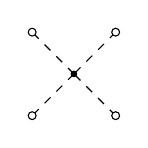
\begin{tikzpicture}[scale=0.5, transform shape]
        \begin{feynman}
            \vertex (a);
            \vertex[below right=of a]  (i2);
            \vertex[below left=of a]  (f2);
            \vertex[above right=of a]  (i1);
            \vertex[above left=of a]  (f1);
            \diagram*{
                (i1) --[scalar] (a) --[scalar] (f2);
                (i2) -- [scalar] (a) -- [scalar] (f1);
            };
            \draw[fill=black] (a) circle(0.7mm);
            \draw[fill=white] (i1) circle(1mm);
            \draw[fill=white] (i2) circle(1mm);
            \draw[fill=white] (f1) circle(1mm);
            \draw[fill=white] (f2) circle(1mm);
        \end{feynman}
    \end{tikzpicture}
\end{figure}

\textbf{Second order:}
\begin{figure}[h]
    \centering
    \begin{tikzpicture}[scale=0.5, transform shape]
        \begin{feynman}
            \vertex (a);
            \vertex[right = of a] (b);
            \vertex[above left = of a] (f1);
            \vertex[below left = of a] (f2);
            \vertex[above right = of b] (i1);
            \vertex[below right = of b] (i2);
            \diagram*{
                (i1) --[scalar] (b);
                (a) --[scalar] (f1);
                (i2) --[scalar] (b);
                (a) --[scalar] (f2);
                (a) --[scalar, half left] (b);
                (a) --[scalar, half right] (b);
            };
            \draw[fill=black] (a) circle(0.7mm);
            \draw[fill=black] (b) circle(0.7mm);
            \draw[fill=white] (i1) circle(0.7mm);
            \draw[fill=white] (i2) circle(0.7mm);
            \draw[fill=white] (f1) circle(0.7mm);
            \draw[fill=white] (f2) circle(0.7mm);
        \end{feynman}
            \node at (4.7,0) {\Huge $+$};
        \begin{scope}[xshift=8cm]
            \begin{feynman}
                \vertex (a);
                \vertex[left = of a] (plus);
                \vertex[above left = of a] (f1);
                \vertex[below left = of a] (f2);
                \vertex[above right = of a] (i1);
                \vertex[below right = of a] (i2);
                \vertex[right = of a] (a1);
                \vertex[right = of a1] (b);
                \vertex[above = of b] (c);
                \vertex[below = of b] (d);
                \diagram*{
                    (i1) --[scalar] (a);
                    (a) --[scalar] (f1);
                    (i2) --[scalar] (a);
                    (a) --[scalar] (f2);
                    (b) --[scalar, half left] (c) --[scalar, half left] (b) --[scalar, half left] (d) --[scalar, half left] (b);
                };
                \draw[fill=black] (a) circle(0.7mm);
                \draw[fill=black] (b) circle(0.7mm);
                \draw[fill=white] (i1) circle(1mm);
                \draw[fill=white] (i2) circle(1mm);
                \draw[fill=white] (f1) circle(1mm);
                \draw[fill=white] (f2) circle(1mm);
            \end{feynman}
        \end{scope}
    \end{tikzpicture}
\end{figure}

\textbf{Third order:}
\begin{figure}[H]
    \centering
    \begin{tikzpicture}[scale=0.5, transform shape]
        \begin{feynman}
            \vertex (a);
            \vertex[right = of a] (b);
            \vertex[right = of b] (c);
            \vertex[above left = of a] (f1);
            \vertex[below left = of a] (f2);
            \vertex[above right = of c] (i1);
            \vertex[below right = of c] (i2);
            \diagram*{
                (i1) --[scalar] (c);
                (a) --[scalar] (f1);
                (i2) --[scalar] (c);
                (a) --[scalar] (f2);
                (a) --[scalar, half left] (b);
                (b) --[scalar, half left] (c);
                (a) --[scalar, half right] (b);
                (b) --[scalar, half right] (c);
            };
            \draw[fill=black] (a) circle(0.7mm);
            \draw[fill=black] (b) circle(0.7mm);
            \draw[fill=black] (c) circle(0.7mm);
            \draw[fill=white] (i1) circle(1mm);
            \draw[fill=white] (i2) circle(1mm);
            \draw[fill=white] (f1) circle(1mm);
            \draw[fill=white] (f2) circle(1mm);
        \end{feynman}
            \node at (5.4,0) {\Huge $+$};
        \begin{scope}[xshift=8cm]
            \begin{feynman}
                \vertex (a);
                \vertex[right = of a] (b);
                \vertex[above left = of a] (f1);
                \vertex[below left = of a] (f2);
                \vertex[above right = of b] (i1);
                \vertex[below right = of b] (i2);
                \vertex[right = of b] (b1);
                \vertex[right = of b1] (c);
                \vertex[above = of c] (d);
                \vertex[below = of c] (e);
                \diagram*{
                    (i1) --[scalar] (b);
                    (a) --[scalar] (f1);
                    (i2) --[scalar] (b);
                    (a) --[scalar] (f2);
                    (a) --[scalar, half left] (b);
                    (a) --[scalar, half right] (b);
                    (c) --[scalar, half left] (d) --[scalar, half left] (c) --[scalar, half left] (e) --[scalar, half left] (c);

                };
                \draw[fill=black] (a) circle(0.7mm);
                \draw[fill=black] (b) circle(0.7mm);
                \draw[fill=black] (c) circle(0.7mm);
                \draw[fill=white] (i1) circle(1mm);
                \draw[fill=white] (i2) circle(1mm);
                \draw[fill=white] (f1) circle(1mm);
                \draw[fill=white] (f2) circle(1mm);
            \end{feynman}
        \end{scope}
            \node at (14.5,0) {\Huge $+$};

        \begin{scope}[xshift=17cm]
            \begin{feynman}
                \vertex (a);
                \vertex[left = of a] (plus);
                \vertex[above left = of a] (f1);
                \vertex[below left = of a] (f2);
                \vertex[above right = of a] (i1);
                \vertex[below right = of a] (i2);
                \vertex[right = of a] (a1);
                \vertex[right = of a1] (b);
                \vertex[above = of b] (c);
                \vertex[below = of b] (d);
                \vertex[right = of b] (b1);
                \vertex[right = of b1] (e);
                \vertex[above = of e] (f);
                \vertex[below = of e] (g);
                \diagram*{
                    (i1) --[scalar] (a);
                    (a) --[scalar] (f1);
                    (i2) --[scalar] (a);
                    (a) --[scalar] (f2);
                    (b) --[scalar, half left] (c) --[scalar, half left] (b) --[scalar, half left] (d) --[scalar, half left] (b);
                    (e) --[scalar, half left] (f) --[scalar, half left] (e) --[scalar, half left] (g) --[scalar, half left] (e);
                };
                \draw[fill=black] (a) circle(0.7mm);
                \draw[fill=black] (b) circle(0.7mm);
                \draw[fill=black] (e) circle(0.7mm);
                \draw[fill=white] (i1) circle(1mm);
                \draw[fill=white] (i2) circle(1mm);
                \draw[fill=white] (f1) circle(1mm);
                \draw[fill=white] (f2) circle(1mm);
            \end{feynman}
        \end{scope}
            
        \node at (25.2,0) {\Huge $+$};

        \begin{scope}[xshift=28cm]
            \begin{feynman}
                \vertex (a);
                \vertex[above left = of a] (f1);
                \vertex[below left = of a] (f2);
                \vertex[above right = of a] (i1);
                \vertex[below right = of a] (i2);
                \diagram*{
                    (i1) --[scalar] (a);
                    (a) --[scalar] (f1);
                    (i2) --[scalar] (a);
                    (a) --[scalar] (f2);
                };
                \draw[fill=black] (a) circle(0.7mm);
                \draw[fill=white] (i1) circle(1mm);
                \draw[fill=white] (i2) circle(1mm);
                \draw[fill=white] (f1) circle(1mm);
                \draw[fill=white] (f2) circle(1mm);
            \end{feynman}
        \end{scope}
        \begin{scope}[xshift=31.5cm, yshift=0.75cm]
            \begin{feynman}
                \vertex (a);
                \vertex[above = of a] (u);
                \vertex[below = of a] (b);
                \vertex[below = of b] (d);
                \diagram*{
                    (u) --[scalar, half left] (a) --[scalar, half left] (b)--[scalar, half left] (d) --[scalar, half left] (b)--[scalar, half left] (a)--[scalar, half left] (u);
                };
                \draw[fill=black] (a) circle(0.7mm);
                \draw[fill=black] (b) circle(0.7mm);
            \end{feynman}
        \end{scope}
    \end{tikzpicture}
\end{figure}

and so on.\\
%  (notice that there are still other disconnected diagrams such as the following, at all orders
% \begin{figure}[H]
%     \centering
%     \begin{tikzpicture}[scale=0.5, transform shape]
%         \begin{feynman}
%             \vertex (a);
%             \vertex[below right=of a]  (i2);
%             \vertex[below left=of a]  (f2);
%             \vertex[above right=of a]  (i1);
%             \vertex[above left=of a]  (f1);
%             \vertex[right = of a] (a1);
%             \vertex[right = of a1] (a2);
%             \diagram*{
%                 (f1) --[scalar] (f2);
%                 (i1) -- [scalar] (a1) -- [scalar] (i2);
%                 (a1) --[scalar, half left] (a2) --[scalar, half left] (a1);

%             };
%             \draw[fill=black] (a1) circle(0.7mm);
%             \draw[fill=black] (i1) circle(0.7mm);
%             \draw[fill=black] (i2) circle(0.7mm);
%             \draw[fill=black] (f1) circle(0.7mm);
%             \draw[fill=black] (f2) circle(0.7mm);
%         \end{feynman}
%     \end{tikzpicture}
% \end{figure}

% which arose from contractions of the form \(\wick{\c\phi(x_1)\c\phi(x_2)\c\phi(x_3)\c\phi(x)\c\phi(x_4)\c\phi(x)\c\phi(x)\c\phi(x)}\) . We are conveniently ignoring these diagrams right now, since the final result we are trying to demonstrate holds even with these diagrams.)\\

If we collect together the subdiagrams which have all the lines connected to external legs and call them connected diagrams,
\begin{figure}[H]
    \centering
    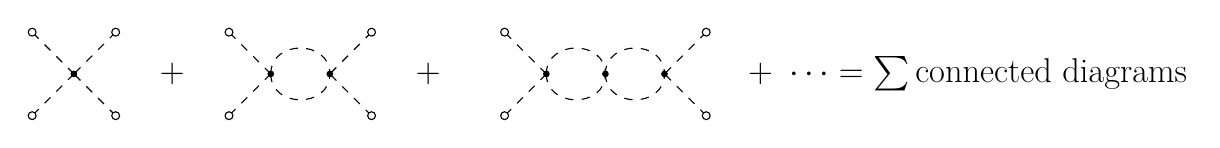
\begin{tikzpicture}[scale=0.5, transform shape]
        \begin{feynman}
            \vertex (a);
            \vertex[right = of a] (b);
            \vertex[right = of b] (c);
            \vertex[above left = of a] (f1);
            \vertex[below left = of a] (f2);
            \vertex[above right = of c] (i1);
            \vertex[below right = of c] (i2);
            \diagram*{
                (i1) --[scalar] (c);
                (a) --[scalar] (f1);
                (i2) --[scalar] (c);
                (a) --[scalar] (f2);
                (a) --[scalar, half left] (b);
                (b) --[scalar, half left] (c);
                (a) --[scalar, half right] (b);
                (b) --[scalar, half right] (c);
            };
            \draw[fill=black] (a) circle(0.7mm);
            \draw[fill=black] (b) circle(0.7mm);
            \draw[fill=black] (c) circle(0.7mm);
            \draw[fill=white] (i1) circle(1mm);
            \draw[fill=white] (i2) circle(1mm);
            \draw[fill=white] (f1) circle(1mm);
            \draw[fill=white] (f2) circle(1mm);
        \end{feynman}
            \node at (-3,0) {\Huge $+$};
        \begin{scope}[xshift=-7cm]
            \begin{feynman}
                \vertex (a);
                \vertex[right = of a] (b);
                \vertex[above left = of a] (f1);
                \vertex[below left = of a] (f2);
                \vertex[above right = of b] (i1);
                \vertex[below right = of b] (i2);
                \vertex[right = of b] (b1);
                \vertex[right = of b1] (c);
                \vertex[above = of c] (d);
                \vertex[below = of c] (e);
                \diagram*{
                    (i1) --[scalar] (b);
                    (a) --[scalar] (f1);
                    (i2) --[scalar] (b);
                    (a) --[scalar] (f2);
                    (a) --[scalar, half left] (b);
                    (a) --[scalar, half right] (b);

                };
                \draw[fill=black] (a) circle(0.7mm);
                \draw[fill=black] (b) circle(0.7mm);
                \draw[fill=white] (i1) circle(1mm);
                \draw[fill=white] (i2) circle(1mm);
                \draw[fill=white] (f1) circle(1mm);
                \draw[fill=white] (f2) circle(1mm);
            \end{feynman}
        \end{scope}
            \node at (-9.5,0) {\Huge $+$};
        \begin{scope}[xshift=-12cm]
            \begin{feynman}
                \vertex (a);
                \vertex[left = of a] (plus);
                \vertex[above left = of a] (f1);
                \vertex[below left = of a] (f2);
                \vertex[above right = of a] (i1);
                \vertex[below right = of a] (i2);
                \vertex[right = of a] (a1);
                \vertex[right = of a1] (b);
                \vertex[above = of b] (c);
                \vertex[below = of b] (d);
                \vertex[right = of b] (b1);
                \vertex[right = of b1] (e);
                \vertex[above = of e] (f);
                \vertex[below = of e] (g);
                \diagram*{
                    (i1) --[scalar] (a);
                    (a) --[scalar] (f1);
                    (i2) --[scalar] (a);
                    (a) --[scalar] (f2);
                };
                \draw[fill=black] (a) circle(0.7mm);
                \draw[fill=white] (i1) circle(1mm);
                \draw[fill=white] (i2) circle(1mm);
                \draw[fill=white] (f1) circle(1mm);
                \draw[fill=white] (f2) circle(1mm);
            \end{feynman}
        \end{scope}
        \node at (10.7,0) {\Huge $ + ~\cdots = \sum \text{connected diagrams}$};
    \end{tikzpicture}
\end{figure}
and the subdiagrams where there are no external legs at all the disconnected diagrams
\begin{figure}[H]
    \centering
    \begin{tikzpicture}[scale=0.5, transform shape]
        \begin{scope}[xshift=0cm]
            \begin{feynman}
                \vertex (c);
                \vertex[above = of c] (d);
                \vertex[below = of c] (e);
                \diagram*{
                    (c) --[scalar, half left] (d) --[scalar, half left] (c) --[scalar, half left] (e) --[scalar, half left] (c);

                };
                \draw[fill=black] (c) circle(0.7mm);
            \end{feynman}
        \end{scope}
            \node at (2.4,0) {\Huge $+$};
            \node at (-3,0) {\Huge $1~~~+$};

        \begin{scope}[xshift=5cm]
            \begin{feynman}
                \vertex (b);
                \vertex[above = of b] (c);
                \vertex[below = of b] (d);
                \vertex[right = of b] (b1);
                \vertex[right = of b1] (e);
                \vertex[above = of e] (f);
                \vertex[below = of e] (g);
                \diagram*{
                    (b) --[scalar, half left] (c) --[scalar, half left] (b) --[scalar, half left] (d) --[scalar, half left] (b);
                    (e) --[scalar, half left] (f) --[scalar, half left] (e) --[scalar, half left] (g) --[scalar, half left] (e);
                };
                \draw[fill=black] (b) circle(0.7mm);
                \draw[fill=black] (e) circle(0.7mm);
            \end{feynman}
        \end{scope}
            \node at (10.5,0) {\Huge $+$};
        \begin{scope}[xshift=13cm, yshift=0.75cm]
            \begin{feynman}
                \vertex (a);
                \vertex[above = of a] (u);
                \vertex[below = of a] (b);
                \vertex[below = of b] (d);
                \diagram*{
                    (u) --[scalar, half left] (a) --[scalar, half left] (b)--[scalar, half left] (d) --[scalar, half left] (b)--[scalar, half left] (a)--[scalar, half left] (u);
                };
                \draw[fill=black] (a) circle(0.7mm);
                \draw[fill=black] (b) circle(0.7mm);
            \end{feynman}
        \end{scope}
        \node at (15.4,0) {\Huge $+$};
        \begin{scope}[xshift=18.5cm, yshift=1.4cm]
            \begin{feynman}
                \vertex (a);
                \vertex[below= of a] (a1);
                \vertex[below= of a1] (b);
                \diagram* {
                    (a) -- [scalar, bend left=45] (b),
                    (a) -- [scalar, bend left=90, looseness=1.5] (b),
                    (a) -- [scalar, bend right=45] (b),
                    (a) -- [scalar, bend right=90, looseness=1.5] (b),
                };
                \draw[fill=black] (a) circle(0.7mm);
                \draw[fill=black] (b) circle(0.7mm);
            \end{feynman}
        \end{scope}
        \node at (27,0) {\Huge $ + ~\cdots = \sum \text{disconnected diagrams}$};
    \end{tikzpicture}
\end{figure}

then we see that we can factor out the disconnected diagrams from the sum over all the diagrams to give 
\begin{equation*}
    \bra{0}T\left( \phi_I(x_1)\ldots\phi_I(x_n) \left(\e^{-i\int_{-\infty}^{\infty}H_I(t) dt }\right) \right) \ket{0} = \left( \sum \text{connected pieces}  \right) \times \left( \sum \text{disconnected pieces}  \right)
\end{equation*}
The denominator 
\begin{equation*}
    \bra{0}T\left( \e^{-i\int_{-\infty}^{\infty}H_I(t) dt }\right) \ket{0}
\end{equation*}
is nothing but exactly the sum over all disconnected pieces, and therefore we get 
\begin{equation*}
    \bra{\Omega} T\left( \phi_H(x_1),\ldots,\phi_H(x_n)  \right) \ket{\Omega} = \sum \text{connected Feynman diagrams} 
\end{equation*}

(Notice that there are also diagrams of the form 
\begin{figure}[H]
    \centering
    \begin{tikzpicture}[scale=0.5, transform shape]
        \begin{feynman}
            \vertex (a);
            \vertex[below right=of a]  (i2);
            \vertex[below left=of a]  (f2);
            \vertex[above right=of a]  (i1);
            \vertex[above left=of a]  (f1);
            \vertex[right = of a] (a1);
            \vertex[right = of a1] (a2);
            \diagram*{
                (f1) --[scalar] (f2);
                (i1) -- [scalar] (a1) -- [scalar] (i2);
                (a1) --[scalar, half left] (a2) --[scalar, half left] (a1);

            };
            \draw[fill=black] (a1) circle(0.7mm);
            \draw[fill=white] (i1) circle(1mm);
            \draw[fill=white] (i2) circle(1mm);
            \draw[fill=white] (f1) circle(1mm);
            \draw[fill=white] (f2) circle(1mm);
        \end{feynman}
        \node at (-2.5, 0) {\Huge $,$};
        \begin{scope}[xshift=-5cm]
            \begin{feynman}
                \vertex (a);
                \vertex[below right=of a]  (i2);
                \vertex[below left=of a]  (f2);
                \vertex[above right=of a]  (i1);
                \vertex[above left=of a]  (f1);
                \diagram*{
                    (f1) --[scalar] (f2);
                    (i1) -- [scalar] (i2);
                };
                % \draw[fill=black] (a1) circle(0.7mm);
                \draw[fill=white] (i1) circle(1mm);
                \draw[fill=white] (i2) circle(1mm);
                \draw[fill=white] (f1) circle(1mm);
                \draw[fill=white] (f2) circle(1mm);
            \end{feynman}
        \end{scope}
        \node at (-7.5, 0) {\Huge $,$};
        \begin{scope}[xshift=-10cm]
            \begin{feynman}
                \vertex (a);
                \vertex[below right=of a]  (i2);
                \vertex[below left=of a]  (f2);
                \vertex[above right=of a]  (i1);
                \vertex[above left=of a]  (f1);
                \diagram*{
                    (f1) --[scalar] (i1);
                    (f2) -- [scalar] (i2);
                };
                % \draw[fill=black] (a1) circle(0.7mm);
                \draw[fill=white] (i1) circle(1mm);
                \draw[fill=white] (i2) circle(1mm);
                \draw[fill=white] (f1) circle(1mm);
                \draw[fill=white] (f2) circle(1mm);
            \end{feynman}
        \end{scope}
        \node at (5, 0) {\Huge \(,\)~~ etc.};
    \end{tikzpicture}
\end{figure}

at all orders, which might on the surface seem like disconnected diagram, but in-fact are also connected diagrams, since every line is connected to some external line. These diagrams should also be included in the calculation of Green's functions.)\\

The numerator and denominator in the RHS are not something intrinsically meaningful for the theory. It depended on how we chose our vacuum. The fact that this vacuum was not the actual vacuum of the theory is the reason why the disconnected pieces arose. In the Green's function, which is physically meaningful object, all these disconnected diagrams vanish, and only the connected diagrams remain.

\subsection{Another way to interpret the Green's functions}
Consider deforming the Hamiltonian by adding a source to the Hamiltonian 
\begin{equation*}
    H \to H + \int \rho(x) \phi_H(x) d^3\textbf{x}
\end{equation*}
which is equivalent to modifying the Hamiltonian density as 
\begin{equation*}
    \hd \to \hd + \rho(x) \phi_H(x)
\end{equation*}
What this source does is to add some energy proportional to the field, with the proportionality constant depending on spacetime. We can ask now, in the presence of this source, what is the amplitude for the vacuum \(\ket{\Omega}\) back to the original vacuum. To calculate this, we can treat the \(\int \rho(x)\phi_H(x)d^3\textbf{x}\) as the perturbation term, and obtain 
\begin{equation*}
    \bra{\Omega}S_\rho \ket{\Omega} = \bra{\Omega} T\left(\e^{i\int \rho(x)\phi_H(x)d^4x} \right) \ket{\Omega}  = Z[\rho]
\end{equation*}
This is called the vacuum persistance amplitude in the presence of the source \(\rho(x)\), and is sometimes also called the generating function for correlation functions.\\
We can expand the above as 
\begin{equation*}
    Z[\rho] = \sum_n \int d^4x_1 d^4x_2 \ldots d^4x_n \frac{i^n}{n!} \rho(x_1)\rho(x_2)\ldots\rho(x_n)\bra{\Omega} T\left(  \phi_H(x_1)\phi_H(x_2)\cdots \phi_H(x_n) \right) \ket{\Omega}
\end{equation*}
(the time ordering doesn't care about the \(\rho\)s since they are simply functions and not operators.)\\

Now if we take the functional derivative of this generating functional w.r.to the \(\rho(x_i)\)s, 
\begin{equation*}
    (-i)^n\frac{\delta^n Z[\rho]}{\delta \rho(x_1)\delta \rho(x_2) \ldots {\delta \rho(x_n)}} \bigg|_{\rho(x) = 0}= \bra{\Omega} T\left(  \phi_H(x_1)\phi_H(x_2)\cdots \phi_H(x_n) \right) \ket{\Omega}
\end{equation*}
(where the \(n!\) cancelled out since there are \(n!\) ways to act the functional derivatives on the \(n\) terms, and \(\rho(x)=0\) is important to kill off all the terms with power higher than \(n\), which are not killed by the derivative)\\

Therefore, another interpretation of the Green's function is that it tells us how the theory responds to the insertion of a source. The \(Z[\rho]\) is called the ``Generating Function for Correlation Functions'', since it generates the correlation functions for us.

\subsection{LSZ Formula}  
Remember that in the full interacting theory, there is no notion of \textit{one field}, but one is free to redefine the field operators while introducing interaction vertices, which keeps the theory unchanged. This is why we said that the above discussed Green's function was not a good physical question to ask, but rather we should discuss the \(S-\)matrix.
The LSZ formula relates the Greens functions which we have been discussing so far to \(S-\)matrix elements. In Layman language, this formula simply tells to normalise the \(\phi(x)\) correctly, strip off the external propagators, and then put the external momenta on-shell. In the following, we will discuss the same in precise language.\\

First we will have to \textit{define carefully} what an \(S-\)matrix is. So far what we had was some matrix connecting some in-states to some out-states, but we want to make that notion more precise. First of all, let us impose that the fields we want to discuss about must satisfy  
\begin{equation*}
    \bra{\Omega} \phi_H(x) \ket{\Omega} = 0 ~~~~\leftarrow \text{~ subtracting off the vacuum expectation value}
\end{equation*}
and 
\begin{equation*}
    \bra{k} \phi_H(x) \ket{\Omega} = \e^{ik\cdot x}~~~~\leftarrow \text{~ normalising the field}
\end{equation*}
That is, if our original field operators did not satisfy this, then make a field redefinition such that the new fields \(\phi_H(x)\) satisfy the above. We consider these two conditions since the vacuum and the one particle states are special states. The vacuum is the lowest energy state, and the one particle states are also uniquely specified by the conserved energy-momentum charges, and this is true even in the interacting theory. Notice that we have not yet specified what the states \(\ket{k}\) are. The only requirement is that they satisfy \(k^2= m^2\). \\

To calculate the \(S-\)matrix elements, we need some in and out states, to create which, we want to now \textit{extract} something that acts like a ``creation'' operator from the field \(\phi_H(x)\). (This ``creation'' operator will not satisfy the free field algebra, but it will be some operator that will create one particle states). We can do this by using the so-called Klein-Gordon inner product. To do this, we start with \(f(t, \textbf{x})\) that satisfies the Klein-Gordon equation, i.e. 
\begin{equation*}
    \left(-\frac{\del^2}{\del t^2} + \mathbf{\nabla}^2\right)f(t, \textbf{x}) = m^2f(t, \textbf{x})
\end{equation*}
We can now specify if this \(f(t, \textbf{x})\) has only positive or only negative frequencies, and we choose for it to have only negative frequencies. That is 
\begin{equation*}
    f(t, \textbf{x}) = \int \frac{d^3\textbf{k}'}{(2\w_\textbf{k}')(2\pi)^3} f({k}') \e^{-ik'\cdot x}
\end{equation*}
Now consider a smearing of the fields,
\begin{equation*}
    \phi_f(t) = i \int\left[ \phi_H(t, \textbf{x}) \del_0 f(t, \textbf{x}) - \left( \del_0 \phi_H(t, \textbf{x}) \right) f(t, \textbf{x})  \right]d^3\textbf{x}
\end{equation*}
This is called a Klein-Gordon inner product. \\

Now see that 
\begin{equation*}
    \bra{k}\phi_f(t)\ket{\Omega} = i \int \left[  \e^{ik\cdot x} \del_0f(t, \textbf{x}) - i\w_\textbf{k}\e^{ik\cdot x} f(t, \textbf{x})    \right]d^3\textbf{x}
\end{equation*}
substituting the expansion of \(f(t, \textbf{x})\), we get 
\begin{equation*}
    \bra{k}\phi_f(t)\ket{\Omega} = i\int \left[ \e^{ik\cdot x} (-i\w_{\textbf{k}'}) \e^{-ik'\cdot x} + \e^{ik\cdot x} (-i\w_\textbf{k})   \e^{-ik'\cdot x} \right] f({k}') d^3\textbf{x} \frac{d^3\textbf{k}'}{(2\pi)^3(2\w_\textbf{k}')}
\end{equation*}
The integral over \(\textbf{x}\) gives a delta function which sets \(\textbf{k} = \textbf{k}'\). What remains in the exponents is \(\e^{i\w_\textbf{k}t - i\w_\textbf{k}t}\) which again cancel out since both \(\textbf{k}'\) and \(\textbf{k}\) are on-shell, and therefore we are left with 
\begin{equation*}
    \bra{k}\phi_f(t)\ket{\Omega} =  f({k}) 
\end{equation*}
and this is independent of time.\\
A similar calcuation for 
\begin{equation*}
    \bra{\Omega}\phi_f(t)\ket{k}  = i\int \left[ \e^{-ik\cdot x} (-i\w_{\textbf{k}'}) \e^{-ik'\cdot x} + \e^{-ik\cdot x} (i\w_\textbf{k})   \e^{-ik'\cdot x} \right] f({k}') d^3\textbf{x} \frac{d^3\textbf{k}'}{(2\pi)^3(2\w_\textbf{k}')} = 0
\end{equation*}

In a sense, the \(\phi_f\) acts like a ``creation'' operator, which creates the wavepacket given by \(f(k)\). However this is not a creation operator in the sense of a free field creation operator. That is, \(\phi_f(t)\) can also create multi-particle states since the theory is an interacting theory. This is because, for an interacting field 
\begin{equation*}
    \bra{q} \phi_H(x) \ket{\Omega} \ne 0
\end{equation*}
where \(\ket{q}\) is some multiparticle state satisfying \(P_\mu\ket{q} = q_\mu \ket{q}\), since \(\phi_H(x)\) doesn't only contain creation and annihilation operators, but will also have other operators that create multiple particles. Therefore simply smearing this field with some \(f(t, \textbf{x})\) will not end up creating only single particle states, but will also create the multiparticle states.\\

To be precise, let us compute
% \begin{equation*}
%     \bra{q} \phi_f(t) \ket{\Omega} = \int \frac{q_k^0 + \w_\textbf{k}}{2\w_\textbf{k}} \e^{i(q_k^0 - \w_\textbf{k})t}f(k) \frac{d^3\textbf{k}}{(2\pi)^3}
% \end{equation*}
\begin{equation*}
    \bra{q} \phi_f(t) \ket{\Omega}
\end{equation*}
To calculate this, notice that 
\begin{equation*}
    \bra{q} \phi_H(x) \ket{\Omega} = \bra{q}\e^{iP\cdot x} \phi_H(0) \e^{-iP\cdot x}\ket{\Omega}=\e^{iq\cdot x} \bra{q} \phi_H(0) \ket{\Omega}
\end{equation*}
which is given from Lorentz invariance. Therefore 
\begin{equation*}
    \bra{q}\phi_f(t)\ket{\Omega} = i \int \left[  \e^{iq\cdot x} \del_0f(t, \textbf{x}) - iq^0\e^{ik\cdot x} f(t, \textbf{x})    \right]d^3\textbf{x}~\bra{q} \phi_H(0) \ket{\Omega}
\end{equation*}
which gives 
\begin{equation*}
    \bra{q}\phi_f(t)\ket{\Omega} = i\int \left[ \e^{iq\cdot x} (-i\w_{\textbf{k}'}) \e^{-ik'\cdot x} + \e^{iq\cdot x} (-iq^0)   \e^{-ik'\cdot x} \right] f({k}') d^3\textbf{x} \frac{d^3\textbf{k}'}{(2\pi)^3(2\w_\textbf{k}')}~\bra{q} \phi_H(0) \ket{\Omega}
\end{equation*}
Once again we can do the integral over \(\textbf{x}\) to get a delta function \(\textbf{q} = \textbf{k}\). However, now \(q^0 \ne \w_\textbf{q}\) and therefore we will be left with 
\begin{equation*}
    \bra{q}\phi_f(t)\ket{\Omega} = \frac{\w_\textbf{q} + q^0}{2\w_\textbf{q}} \e^{i(q^0 - \w_\textbf{q})t} f(q) \bra{q} \phi_H(0) \ket{\Omega}
\end{equation*}
Now see that this is time dependent and not time independent. Notice that \(q^0 > \w_\textbf{q}\), that is, for a given momentum, a multiparticle state has always more energy than a single particle state
\textcolor{red}{
    \begin{equation*}
        q^0 = \sqrt{\textbf{q}^2 + \sum m_i^2},~~\w_\textbf{q} = \sqrt{\textbf{q}^2 + m^2}
    \end{equation*}
}
and therefore, we get an oscillating phase factor which depends on time. \\

Physically speaking, \(\phi_f(t)\) creates a single particle wavepacket specified by \(f(k)\), and along with that it also creates multiparticle garbage. But we can now see what happens in the limit \(t\to \pm \infty\). Suppose we take a smear the momenta states by considering a superposition of multiparticle states with different momenta and energy, 
\begin{equation*}
    \ket{\psi} \approx \int d^3\textbf{q} g(q) \ket{q}
\end{equation*}
then 
\begin{equation*}
    \lim_{t\to \pm\infty} \bra{\psi}\phi_f(t)\ket{\Omega} \propto \int d^3\textbf{q}~ g(q)\e^{i(q - \w_\textbf{q})t} = 0 
\end{equation*}
Therefore, in the far past and far future, \(\phi_f(t)\) does not create multiparticle states, and the only remaining state is the single particle wavepacket. Physically speaking, \(\phi_f(t)\) creates a wavepacket of single particle states along with some multiparticle garbage states, but if we look at the state \(\phi_f(t)\ket{\Omega}\) in some definite region in space time (i.e.,take its inner product with some definite state \(\ket\psi\)), and send the time of reaction to \(-\infty\), all the multiparticle states will run away. Of course the one particle state may run away too. We prevent this by modifying the state we create in such a way that the single particle wavepacket always has the same relationship to the observer, and that's done by the funny combination \(\phi_f(t)\). No multiparticle state has the right dispersion relation to keep the same relationship to the observer under this modification. \\

To create multiparticle states, we take two different functions \(f_1\) and \(f_2\), and we define a two particle state to be 
\begin{equation*}
    \ket{f_1, f_2}_{\text{in}} = \lim_{t\to -\infty} \phi_{f_1}(t)\phi_{f_2}(t) \ket{\Omega}~~~~{}_{\text{out}}\bra{f_3, f_4} = \lim_{t\to \infty} \bra{\Omega}\phi_{f_3}^\dagger(t)\phi^\dagger_{f_4}(t) 
\end{equation*}
For most choices of \(f_1\) and \(f_2\), we find that the two wavepackets separate at far past and far future. This is because since the wavepackets are headed in different directions in space, in the far past and far future, they are separated well enough that acting \(\phi_{f_2}(t)\) on \(\phi_{f_1}(t)\ket{\Omega}\) will be the same as acting \(\phi_{f_2}(t)\) on the vacuum for a local observer. \\

Notice that even if \(f_1 = f_3\) and \(f_2 = f_4\), the in-states are not the same as out states, since the limits \(t\to+\infty\) and \(t\to -\infty\) of the states are not the same. It does indeed create two particle states, but it is a different two particle states in the in-states and the out-states for the same functions are different. These are the precise in and out states in the full quantum field theory, and the \(S-\)matrix will be the overlap between the two. \\

Therefore, the \(S-\)matrix elements are of the form 
\begin{equation*}
    {}_{\text{out}}\braket{f_3, f_4|f_1, f_2}_{\text{in}} = \lim_{t_1, t_2 \to -\infty}\lim_{t_3,t_4\to \infty} \bra{\Omega} \phi_{f_3}^\dagger(t_3)\phi_{f_4}^\dagger(t_4)\phi_{f_1}(t_1)\phi_{f_2}(t_2)\ket{\Omega}
\end{equation*}
Note that the time ordering is already put in the formula. There is a subtlety regarding the individual time ordering of \(t_1 ~\&~ t_2\), that is, which limit to take first, \(t_1\to -\infty\) or \(t_2\to -\infty\) (and similarly for \(t_3,~t_4\)), but this doesn't matter since the wavepackets are largely separated and therefore they commute. \\

One way to do this would be to explicitly solve for this in \(t\) and take the limit \(t\to \pm \infty\). The LSZ reduction formula gives a convenient way to calculate this without having to go through all that hassle. The formula simply states (for the 4 particle state, this can be generalised to n-particle states too)
\begin{align*}
    &{}_{\text{out}}\braket{f_3, f_4|f_1, f_2}{}_{\text{in}} \\
    &~~~~~~~~~~~~= \int d^4x_1 \ldots d^4x_4 ~f_3^*(x_3)f_4^*(x_4)f_1(x_1)f_2(x_2) \prod_{j=1}^4i\left(\square_j + m^2 \right) \bra{\Omega}T\left\{ \phi_H(x_1)\phi_H(x_2)\phi_H(x_3)\phi_H(x_4) \right\}\ket{\Omega}
\end{align*}
In momentum space 
\begin{equation*}
    \square_j + m^2 \equiv k_j^2 + m^2
\end{equation*}
which would cancel out the external propagators in the Greens function, iff it were a free theory. In the interacting theory it doesn't exactly cancel out the propagator, but the integration over the \(f\)s will put the external momenta on-shell since they are the solutions of the KG equation and they have exactly the momenta that are on-shell. \\
See that the Greens function has poles at all \(k_i^2 = m^2\) if the \(k_i\) are on-shell, and therefore the above procedure simply tells to pick up the residues at these poles. Therefore, \(S-\)matrix is the residue at the poles of the Greens function when the momenta are put on-shell.\\

\underline{Proof}—\\
Before proceeding to the proof, we will prove some intermediate results. First, we want to simplify the following
\begin{align*}
    i\int f(x) (\square + m^2) \phi_H(x) d^4x &= i\int f(x) \left(\del_0^2 - \mathbf{\nabla}^2 + m^2\right)\phi_H(x) d^4x\\
    &=i\int f(x) \del_0^2\phi_H(x) - \left(\mathbf{\nabla}^2 f(x)\right) \phi_H(x) + m^2f(x)\phi_H(x)d^4x
\end{align*}
We are allowed to do this since we assume that \(f(x)\) is a wavepacket of finite extent, and therefore has no support at infinity, therefore the boundary terms are zero.\\
But \(f(x)\) satisfies
\begin{equation*}
    \left(\del_0^2 - \mathbf{\nabla}^2 +m^2\right)f(x) = 0 \implies \left(\mathbf{\nabla}^2 \right)f(x) = (\del_0^2 + m^2)f(x)
\end{equation*}
Therefore, 
\begin{align*}
    i\int f(x) (\square + m^2) \phi_H(x) d^4x &= i\int f(x) \del_0^2\phi_H(x) - \left(\del_0^2 f(x)\right) \phi_H(x)d^4x\\
    &=i\int \del_0\left(f(x) \del_0\phi_H(x)\right) - \del_0\left(\phi_H(x)\del_0 f(x)\right) d^4x\\
    &=\int_{-\infty}^{\infty}\del_0\left(i\int \left(f(x) \del_0\phi_H(x)- \phi_H(x)\del_0 f(x)\right) d^3\textbf{x}\right)dt\\
    &= \int_{-\infty}^{\infty} \del_0\left(- \phi_f(t)\right) dt\\
    &= \phi_f(-\infty) - \phi_f(\infty)
\end{align*}

We have a similar result for \(f^*(x)\),
\begin{equation*}
    i\int f^*(x) (\square + m^2) \phi_H(x) d^4x = \phi_f^\dagger(\infty) - \phi_f^\dagger(-\infty)
\end{equation*}
Notice that the different sign is due to the \(i\to -i\) when \(\phi_f\to \phi^\dagger_f\).\\

With these results, we now proceed to prove the LSZ formula. 
\begin{align*}
    &{}_{\text{out}}\braket{f_3, f_4|f_1, f_2}{}_{\text{in}} \\
    &~~~~~~~~~~~~= \int d^4x_1 \ldots d^4x_4 ~f_3^*(x_3)f_4^*(x_4)f_1(x_1)f_2(x_2) \prod_{j=1}^4i\left(\square_j + m^2 \right) \bra{\Omega}T\left\{ \phi_H(x_1)\phi_H(x_2)\phi_H(x_3)\phi_H(x_4) \right\}\ket{\Omega}
\end{align*}
First, we want to move the \(\square + m^2\) in the LHS into the time ordering. But this is a subtle step since the time ordering has theta functions in time, and the box operator has derivatives w.r.to time.\\

Remember that the difference between one time ordering and another time ordering (i.e.\ \(\phi(x)\phi(y)\) and \(\phi(y)\phi(x)\)) is just the commutator, and it vanishes as long as the points are spacelike separated, and gives something that looks like a delta function in \(x-y\). Therefore, when we take the box operator into the time ordering, we will get some terms where the box operator is acting on the fields, and the other terms will form commutators of the above kind, which are non-zero only in the region where \(x_i ~\&~ x_j\) are close to each other. In the limit where the \(f\)s are orthogonal to each other (i.e. they do not have overlapping support), these terms will identically give \(0\). And therefore, in this limit, it is fine to move the derivatives into the time ordering. \\

\textcolor{red}{
    A rough handwaving argument would be 
    \begin{align*}
        &&\left(\del_0\right)_x \left(\theta(x-y)\phi(x)\phi(y) + \theta(y-x) \phi(y)\phi(x) \right) &= \delta(x-y)\phi(x)\phi(y) - \delta(x-y)\phi(y)\phi(x) + \text{derivative inside T.O.}\\
        && &=\delta(x-y)\left[\phi(x), \phi(y)\right] + \text{derivative inside T.O.}
    \end{align*}
    which implies 
    \begin{align*}
        \left(\del_0^2\right)_x \left(\theta(x-y)\phi(x)\phi(y) + \theta(y-x) \phi(y)\phi(x) \right) &=\del_0\delta(x-y)[\phi(x), \phi(y)] + \delta(x-y)[\Pi(x), \phi(y)] \\
        + \text{derivatives inside T.O.}
    \end{align*}
    The extra terms give zero when the \(f\)s do not have overlapping support.\\
}

After moving the box operators inside and using the above derived relations, we get the following
\begin{align*}
    &{~}_{\text{out}}\braket{f_3, f_4|f_1, f_2}{}_{\text{in}} \\
    &~~~~~= \bra{\Omega} T\left\{  \left(  \phi_{f_1}(-\infty) - \phi_{f_1}(\infty)  \right) \left(  \phi_{f_2}(-\infty) - \phi_{f_2}(\infty)  \right) \left(  \phi^\dagger_{f_3}(\infty) - \phi^\dagger_{f_3}(-\infty)  \right) \left(  \phi^\dagger_{f_4}(\infty) - \phi^\dagger_{f_4}(-\infty)  \right)   \right\} \ket{\Omega}    
\end{align*}
The product will expand to give \(2^4 = 16\) terms, and for each term the time ordering pushes all the \(+\infty\)s to the left and \(-\infty\)s to the right. Let us consider one term of our interest, 
\begin{equation*}
    \bra{\Omega} \phi^\dagger_{f_3}(\infty)\phi_{f_4}^\dagger(\infty) \phi_{f_1}(-\infty)\phi_{f_2}(-\infty)\ket{\Omega}
\end{equation*}
which is exactly equal to 
\begin{equation*}
    {~}_{\text{out}}\braket{f_3, f_4|f_1, f_2}{}_{\text{in}}
\end{equation*}
Therefore, it should be true that all other \(15\) terms are zero. To see why, let us look at some other term 
\begin{equation*}
    \bra{\Omega} \phi_{f_1}(\infty)\phi_{f_2}(\infty)\phi^\dagger_{f_3}(-\infty)\phi_{f_4}^\dagger(-\infty) \ket{\Omega}
\end{equation*}
This term is zero, since \(\phi_f^\dagger\) is an annihilation operator, and therefore gives zero. 
Another term would be of the form 
\begin{equation*}
    \bra{\Omega} \phi^\dagger_{f_3}(\infty)\phi_{f_2}(\infty) \phi_{f_1}(-\infty)\phi_{f_4}^\dagger(-\infty)\phi_{f_2}(-\infty)\ket{\Omega}    
\end{equation*}
There is an subtlety in this, a question if one can commute the \(\phi_{f_i}^\dagger\)s with the \(\phi_{f_j}\)s to annihilate the vacuum, and the answer is that we can indeed commute them since at \(\pm\infty\) the wavepackets are well separated, therefore giving the above term also to be 0. Similarly all other 13 terms give 0, and we have proved the LSZ formula.\\

There are other ways to derive this formula, which would roughly be to start with this definition 
\begin{equation*}
    {~}_{\text{out}}\braket{f_3, f_4|f_1, f_2}{}_{\text{in}} = \bra{\Omega} \phi^\dagger_{f_3}(\infty)\phi_{f_4}^\dagger(\infty) \phi_{f_1}(-\infty)\phi_{f_2}(-\infty)\ket{\Omega}
\end{equation*}
and then argue that by taking the times to infinty, we pick the poles of the Green's function, and when we strip off the poles, we get the \(S-\)matrix. This approach can be found in Peskin and Schroeder, and we do not discuss this here. \\

A very important point — in the LSZ reduction formula, what is the \(\phi_H\) that goes into its definition? There is no consensus on what should be the unique field in an interacting theory, and different field redefinitions give different interactions. In principle any redefinition is also a good definition for the theory, and in deriving the LSZ reduction formula, we never required that the \(\phi_H\) was an elementary field, i.e.\ the field that enters the free Lagrangian. The LSZ formula works with any \underline{operators \(Q(x)\)}, as long as they satisfy the normalisation condition
\begin{equation*}
    \bra{k}Q(x)\ket{\Omega} = \e^{ik\cdot x}
\end{equation*} 
For instance, lets say we want to compute the \(S-\)matrix for some bound state. We do not have ``fields'' which create these bound states, but we can still compute the \(S-\)matrix for those bound states by the virtue that if the bound state is a stable state, then there should be some operator that has the above discussed overlap with the one-particle bound state, and we can calculate the \(S-\)matrix from that. \\




\newpage
\section{Loop Amplitudes and Renormalisation}
Consider a simple second order diagram in the calculation of \(4-\)point function in the \(\phi^4\) theory. 
\begin{figure}[h]
    \centering
    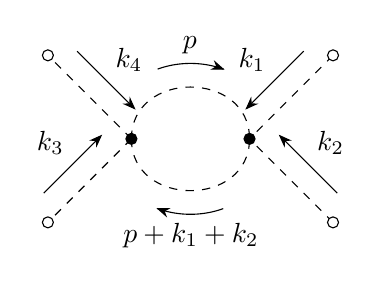
\begin{tikzpicture}[scale=1]
        \begin{feynman}
            \vertex (a);
            \vertex[right = of a] (b);
            \vertex[above left = of a] (f1);
            \vertex[below left = of a] (f2);
            \vertex[above right = of b] (i1);
            \vertex[below right = of b] (i2);
            \diagram*{
                (i1) --[scalar, momentum'=\(k_1\)] (b);
                (a) --[scalar, rmomentum'=\(k_4\)] (f1);
                (i2) --[scalar, momentum'=\(k_2\)] (b);
                (a) --[scalar, rmomentum'=\(k_3\)] (f2);
                (a) --[scalar, half left, momentum={[arrow shorten=0.35]\(p\)}] (b);
                (a) --[scalar, half right, rmomentum'={[arrow shorten=0.35]\(p + k_1 + k_2\)}] (b);
            };
            \draw[fill=black] (a) circle(0.7mm);
            \draw[fill=black] (b) circle(0.7mm);
            \draw[fill=white] (i1) circle(0.7mm);
            \draw[fill=white] (i2) circle(0.7mm);
            \draw[fill=white] (f1) circle(0.7mm);
            \draw[fill=white] (f2) circle(0.7mm);
        \end{feynman}
    \end{tikzpicture}
\end{figure}

This will have an overall energy-momentum conserving delta function, but there is no restriction on \(p\), that is, any value of \(p\) will satisfy the energy-momentum conservation. Therefore, the above diagram will have propagators
\begin{equation*}
    \int d^4p \frac{1}{p^2 - m^2 + i\epsilon}\times \frac{1}{(p+k_1+k_2)^2 - m^2 + i\epsilon}
\end{equation*}
and since there is no restrictions on \(p\) in the form of some delta functions, the above integral is divergant.\\

It is common in field theories that as we go to diagrams with loops, they diverge, and this divergence is not because we were wrong in our definitions, but rather it has to attribute to the fact that we are not being precise with what are the limits of our theory and what questions we can really ask. The quantum field theory we are discussing is, in a sense an \textit{effective field theory} of an underlying ``ultimate'' description of the microscopic scales. (This statement is true in almost every physical theories, we do not model the flow of a liquid based on the movements of the individual particles in it, and similarly in the case of field theories). At long distances, the microscopic parameters combine in some way to give us some ``physical'' observables, and the effective field theory relates one set of physical observables to another set of physical observables. If we try to directly relate the physical observables we have, to the microscopic parameters, then the relationship will be complicated, giving all sorts of divergences. The field theory we have is a good description of physics at scales only larger than some length scale, and the above infinity arises because we wrongly assume that our effective field theory is valid also in scales smaller than this. To be precise, the above divergence arose because we allowed arbitrarily large momenta to circulate in our loop (remember that higher the energy of a process, the smaller the scale probed).\\

An important question one would therefore ask is how would the various parameters in the Lagrangian grow and decay with energy. As said, there might be some parameters in the complete theory, and what we see in the experiments will be some low energy effective parameters. Some basic dimensional analysis will allow us to determine what are the possible low energy effective parameters that we can consider in our field theories.

\subsection{Dimensional Analysis}
In the units we have chosen, \(\hbar = c = 1\), since action has the same dimensions as \(\hbar\), we have 
\begin{equation*}
    [S] = 1 \implies [L] = M^{-1}
\end{equation*}
Therefore, for an arbitray interacting scalar field theory 
\begin{equation*}
    S = \int d^4x \frac{1}{2}(\del_\mu \phi(x))^2 - \frac{m^2}{2}\phi(x)^2 + \sum_{n\ge 3}\frac{\lambda_n}{n!}\phi(x)^n
\end{equation*}
should be dimensionless, and the first term gives
\begin{equation*}
    [x]^4[x]^{-2}[\phi]^2 = 1 \implies [\phi]= L^{-1} = M
\end{equation*}
Given this, we can now ask what are the dimensions of the various parameters that arise in the Lagrangian density. See that 
\begin{equation*}
    [m] = [M]
\end{equation*}
and
\begin{equation*}
    [\lambda_n] = \frac{L^n}{L^4} = L^{n-4} = M^{4-n}
\end{equation*}
We now ask what happens to the different parameters at different energy scales. To answer the question of scales, we always need to consider dimensionless quantities, since the notion of large/small does not make sense for dimensionful quantities. Therefore, for a given parameter, at an energy scale \(E\sim \Lambda\) we need to form a dimensionless quantities. \\

For \(m\) the dimensionless quantity would be 
\begin{equation*}
    \frac{m}{\Lambda}
\end{equation*}
and this becomes small at high energies and large at low energies. This kind of parameter is called ``relevant parameter''. \\
For the other couplings, the dimensionless quantities are 
\begin{equation*}
    \frac{\lambda_n}{\Lambda^{4-n}}
\end{equation*}
and we see that for \(n=3\) this is again a relevant parameter. \\
For \(n>4\), we see that the dimensionless parameter is 
\begin{equation*}
    \lambda_n \Lambda^{n-4}
\end{equation*}
which becomes large at large energies and small at low energies, and this kind of parameter is called ``irrelevant'' since it does not have any effect on our effective field theoretical descriptions at low energies. An example of irrelevant coupling in nature would be gravity, since 
\begin{equation*}
    G_N \propto \frac{1}{L_{\text{Planck}}^2} \implies G_N\Lambda^2
\end{equation*} is the dimensionless parameter. \\

In the case of \(n=4\), the parameter is dimensionless, and therefore this does not scale with energy at all, it is relevant at all energy scales. This is called ``marginal parameter''. Now when we add quantum effects, this properties can change, and the coupling can become marginally relevant or marginally irrelevant. We will see later that in the \(\phi^4\) theory, the coupling becomes marginally irrelevant.

\subsection{Renormalisation}

Theories that have marginal and relevant parameters are called \textit{renormalisable theories}, while theories with irrelevant parameters are called \textit{non-renormalisable theories}. Physically, this is because the parameters that grow large with energy are sensitive to what happens at high energies, and we therefore cannot define a \textit{UV completion} of the theory by introducing some mathematical guesswork. But in the case for theories with only relevant and marginal parameters, we can define some UV completion for the theory, without affecting the details of the low energy theory at all. What renormalisation does is completes the UV physics by  making some guess, which might not be the way the physical things works, while being rest assured that the low energy physics is unaltered.
Operationally what this tells us is that the \(\ld\) is the bare Lagrangian, and we should adjust its parameters in the correct way to get the low-energy physics. That is, in 
\begin{equation*}
    \ld = \frac{1}{2}(\del_\mu \phi)^2 - \frac{m^2}{2}\phi^2 + \frac{\lambda}{4!}\phi^4
\end{equation*}
the parameters \(m\) and \(\lambda\) are not the parameters we can obtain from the low energy experiments. Therefore, we should write a counterterm lagrangian which might have different parameters, so that the above \(m\) and \(\lambda\) are now the parameters we measure in low-energy experiments. 

For the \(\phi^4\) theory, the counterterm lagrangian would be 
\begin{equation*}
    \ld_{\text{CT}} = A\phi + \frac{B}{2}(\del_\mu \phi)^2 - \frac{C}{2}\phi^2  + \frac{D}{4!}\phi^4
\end{equation*}
and we fix the parameters \(A,~B,~C,~D\) by the low energy physical data. What are the possible physical data? For example, we could have (Note:- from now on \(\ket{0}\) will unambigously mean the vacuum of the full Hamiltonian and not the free vacuum, since we will not invoke the free theory vacuum any more in our discussions.)
\begin{equation*}
    \bra{0}\phi(x)\ket{0} = 0,~~\bra{k}\phi(x)\ket{0} = \e^{ik\cdot x}
\end{equation*}
and we can use these to fix the parameters \(A\) and \(B\) of the counterterm lagrangian. Further, we can require the mass of the excitation to be \(m\) which will fix \(C\), and then we can also get the amplitude for some low energy scattering which would also fix \(D\).\\

For the scalar Yukawa theory with 
\begin{equation*}
    \ld = |\del_\mu \psi|^2 + \frac{1}{2}(\del_\mu \phi)^2 - \frac{m^2}{2}\phi^2 - M^2|\psi|^2 - g\phi|\psi|^2
\end{equation*}
the counterterm Lagrangian would be 
\begin{equation*}
    \ld_{\text{CT}} = A\phi + \frac{B}{2}(\del_\mu \phi)^2 + \frac{C}{2}\phi^2 + D|\del_\mu \psi|^2  + E|\psi|^2 - F\phi|\psi|^2
\end{equation*}
Notice that there is no term proportional to \(\psi\), since a) the Lagrangian density should be a real function, and b) the theory has \(SO(2)\) symmetry in \(\psi-\psi^\dagger\), and the counterterm Lagrangian should follow the symmetry too.\\
The physical requirements area
\begin{itemize}
    \item \(\bra{0}\phi\ket{0} 0 \to~A\)
    \item \(\bra{q}\phi(x)\ket{0} = \e^{iq\cdot x} \to B\)
    \item \(\bra{p}\psi(x)\ket{0} = \e^{ip\cdot x} \to D\)
    \item Mass of \(\phi = m \to C\)
    \item Mass of \(\psi = M \to E\)
    \item \(g\) matches the scattering amplitude of some low energy scattering \(\to F\) 
\end{itemize}

Let us make some of these more formal and precise and then work out what the counter terms are. \\

First let us look at the counterterm \(A\phi\). The vertex for it would be simply a linear vertex (we are using \(\times\) to denote the \(A\) vertex)
\begin{figure}[h]
    \centering
    \begin{tikzpicture}
        \begin{feynman}
            \vertex (a);
            \vertex[right= of a] (b);
            \diagram*{
                (b) --[scalar] (a)
            };
            \node at (b) {\(\boldsymbol{\times}\)};  
        \end{feynman}
    \end{tikzpicture}
\end{figure}

The condition that \(\braket{0|\phi(x)|0}\) simply implies that 
\begin{figure}[h]
    \centering
    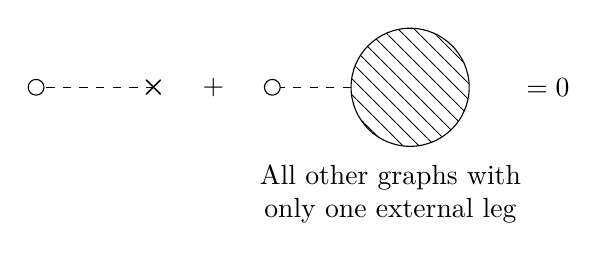
\begin{tikzpicture}
        \begin{feynman}
            \vertex (a);
            \vertex[right= of a] (b);
            \diagram*{
                (b) --[scalar] (a)
            };
            \node at (b) {\(\boldsymbol{\times}\)}; 
            \draw[fill=white] (a) circle(1mm); 
        \end{feynman}
        \node at (2.25,0) {\(+\)};
        \begin{scope}[xshift=3cm]
            \begin{feynman}
                \vertex (a) at (0,0);
                \vertex (b) at (1,0);
                \diagram*{
                    (b) --[scalar] (a)
                };
                \draw[pattern={Lines[angle=-45,distance=4pt]}] (1.75,0) circle(0.75cm) ;
                \draw[fill=white] (a) circle(1mm); 
            \end{feynman}
            \node at (3.5,0) {\(=0\)};
            \node[align=center, text width=4cm] at (1.5, -1.35) {All other graphs with only one external leg};
        \end{scope}
    \end{tikzpicture}
\end{figure}

What this means is that we never have to calculate what \(A\) actually is, all \(A\) does is sets such graphs to zero. \\ 

A similar argument holds in the scalar Yukawa theory too, and in the Yukawa theory, the term sets the diagrams of the following kind to zero. (we did not give explicit example in \(\phi^4\) theory because there are no simple such diagrams in this theory)
\begin{figure}[h]
    \centering
    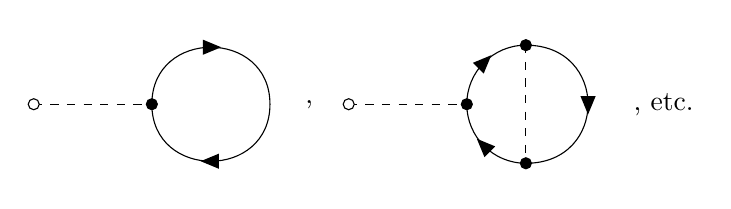
\begin{tikzpicture}
        \begin{feynman}
            \vertex (a);
            \vertex[right = of a] (b);
            \vertex[right = of b] (c);
            \diagram*{
                (a) --[scalar] (b);
                (b) --[fermion, half left, looseness=1.65] (c);
                (c) --[fermion, half left, looseness=1.65] (b);
            };
        \end{feynman}
        \draw[fill=white] (a) circle(0.7mm); 
        \draw[fill=black] (b) circle(0.7mm); 
        \node at (3.5,0) {,};
        \begin{scope}[xshift=4cm]
            \begin{feynman}
            \vertex at (0,0) (a);
            \vertex at (1.5, 0) (b);
            \vertex at (3,0) (c);
            \vertex at (2.25, 0.75) (mu);
            \vertex at (2.25, -0.75) (md);
            \diagram*{
                (a) --[scalar] (b);
                (b) --[fermion, quarter left, looseness=1] (mu);
                (md) --[fermion, quarter left, looseness=1] (b);
                (mu) -- [scalar] (md);
                (mu) --[fermion, half left, looseness=1.8] (md);
            };
        \end{feynman}
        \draw[fill=white] (a) circle(0.7mm); 
        \draw[fill=black] (b) circle(0.7mm); 
        \draw[fill=black] (mu) circle(0.7mm); 
        \draw[fill=black] (md) circle(0.7mm); 
        \end{scope}
        \node at (8,0) {,~etc.};
    \end{tikzpicture}
\end{figure}

Such diagrams, which have only one external point and have multiple internal vertex are called tadpoles and our renormalisation procedure tells us that they can be neglected.\\

\textcolor{red}{
    In the bare theory there also arises uncontrollable infinities in the form of the tadpole diagrams. As an example, consider the 3-point function in the scalar Yukawa theory, with one internal vertex. So far we have only seen the following diagram 
    \begin{figure}[h]
        \centering
        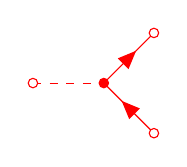
\begin{tikzpicture}[color=red, scale=0.6, transform shape]
            \begin{feynman}
                \vertex (im);
                \vertex[right = of im] (v);
                \vertex[above right = of v] (in);
                \vertex[below right = of v] (inb);
                \diagram*{
                    (im) --[scalar] (v);
                    (v) --[fermion] (in);
                    (inb) --[fermion] (v);
                };
            \end{feynman}
            \draw[fill=white] (im) circle(1mm); 
            \draw[fill=white] (in) circle(1mm); 
            \draw[fill=white] (inb) circle(1mm); 
            \draw[fill=red] (v) circle(1mm); 
        \end{tikzpicture}
    \end{figure}\\
    which was finite. But there are also divergant diagrams of the following form
    \begin{figure}[h]
    \centering
    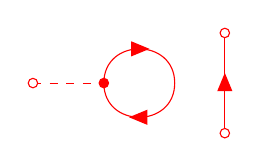
\begin{tikzpicture}[color=red, scale=0.6, transform shape]
        \begin{feynman}
            \vertex (a);
            \vertex[right = of a] (b);
            \vertex[right = of b] (c);
            \vertex[above right = of c] (n);
            \vertex[below right = of c] (nb);
            \diagram*{
                (a) --[scalar] (b);
                (b) --[fermion, half left, looseness=1.65] (c);
                (c) --[fermion, half left, looseness=1.65] (b);
                (nb) --[fermion] (n);
            };
        \end{feynman}
        \draw[fill=white] (a) circle(1mm); 
        \draw[fill=white] (nb) circle(1mm); 
        \draw[fill=white] (n) circle(1mm); 
        \draw[fill=red] (b) circle(1mm); 
    \end{tikzpicture}
\end{figure}\\
which contribute to the 3-point function.\\
Without the term \(A\phi(x)\), the quantity \(\braket{0|\phi(x)|0}\) would be some infinity which is given by the sum of all the tadpole diagrams. But introducing the extra term linear in \(\phi\) allows us to set the value of \(A\) such that the extra vertex that we get from \(A\phi(x)\) exactly cancels out all these infinities, allowing us to set \(\braket{0|\phi(x)|0} = 0\). What this means for the perturbation expansion for the \(S-\)matrix is that one can conveniently ignore all the terms which have the tadpole diagrams knowing that the extra vertex due to \(A\) should also be included, and it will inevitable cancel these infinities.\\
}

Lets now consider the other two conditions \(\braket{q|\phi(x)|0} = \e^{iq\cdot x}\)
and that the mass \(m\) should be the physical mass. \\

Before discussing them, we want to reframe these conditions in terms of the propagator 
\begin{equation*}
    G(x,y) = \bra{0} T\left\{ \phi(x) \phi(y) \right\}\ket{0}
\end{equation*}
We will prove two results about this propagator, the first one being the K\"all\'en-Lehmann spectral representation theorem, and the other being a concept of self-energy, and in terms of these we will discuss these renormalisation conditions.\\

\underline{K\"all\'en-Lehmann spectral representation theorem}\\
First start with the above propagator and insert identity in the form of a complete set of eigenstates, 
\begin{equation*}
    G(x,y) = \theta(x_0-y_0)\sum_{E} \bra{0} \phi(x) \ket{E}\bra{E} \phi(y) \ket{0} + ~y_0>x_0\text{ term}
\end{equation*}
There will be a vacuum state in the complete set, which will give zero owing to our above condition. The first contribution we get will come from single particle states, which would be 
\begin{equation*}
    \sum_{\textbf{k}} \bra{0}\phi(x)\ket{{k}}\bra{{k}}\phi(y)\ket{0} + ~\text{the other term}
\end{equation*}
We know what the measure for the momentum intergration is, and we can indeed perform this summation (integration). If the renormalisation condition we required above is to be true, then we know that this is simply 
\begin{equation*}
    \int \frac{d^3\textbf{k}}{(2\pi)^3 2\w_\textbf{k}} \left( \theta(x_0 - y_0)\e^{-ik(x-y)} + \theta(y_0 - x_0)\e^{-ik(y-x)} \right)
\end{equation*}
which is just the usual free field propagator.\\
The other terms, which would be the contribution from the multi-particle states, would look like 
\begin{equation*}
    \sum_{n\notin \text{s.p.\ states}} \left( \theta(x_0>y_0) \e^{-iQ_n(x-y)}|\braket{0|\phi(0)|n}|^2  + ~y_0>x_0\text{~term}\cdots\right)
\end{equation*}
In the free field theory such terms never arose since the field \(\phi\) had no overlap between the vacuum and multiparticle states. \(\phi\) always created only single particle states in the free theory. But this is not the case in the interacting theory. We do not know how to write this since we do not know what the measure is, and we also do not know any conditions what the elements \(\braket{0|\phi(0)|n}\) should be.\\

We can put this in some nice form by looking at the Fourier transform (calling \(z=y-x\))
\begin{equation*}
    \sum_{n\notin \text{s.p.\ states}}\int d^4z ~\e^{-ipz}~ \e^{iQ_nz}|\braket{0|\phi(0)|n}|^2 = \sum_{n\notin \text{s.p.\ states}} \delta^4(p-Q_n)~|\braket{0|\phi(0)|n}|^2
\end{equation*}
This only depends on \(p\) since everythin else is getting summed over. But this is a Lorentz invariant object, and therefore whatever \(p\) dependence exists should be of the form \(\sigma(p^2)\), i.e. 
\begin{equation*}
    \sum_{n\notin \text{s.p.\ states}} \delta^4(p-Q_n)~|\braket{0|\phi(0)|n}|^2 = \sigma(p^2)
\end{equation*}
Notice that since \(Q_n^2 > m^2\), and therefore \(\sigma(p^2)\) has no support for \(p^2< m^2\), i.e. \(p^2<m^2 \implies \sigma(p^2) = 0\). Further \(\sigma(p^2)\) should be positive, since we are summing over the square of absolute values, which are all positive.\\
Therefore we get 
\begin{equation*}
    \sum_{n\notin \text{s.p.\ states}}\e^{-iQ_n(x-y)}|\braket{0|\phi(0)|n}|^2 = \int \e^{ipz} \sigma(p^2) \frac{d^4p}{(2\pi)^4}, ~~~~~\sigma(p^2)\ge 0,~\sigma(p^2)|_{p^2<m^2} = 0
\end{equation*}
We can now insert a \(1\) in the above term as
\begin{equation*}
    \int \e^{ipz} \sigma(p^2) ~(2\pi)\delta(p^2-a^2) \frac{da^2}{(2\pi)} ~\frac{d^4p}{(2\pi)^4}
\end{equation*}
and we can switch the order of integration, giving 
\begin{equation*}
    \int \left(\int  \e^{ipz} \sigma(p^2) ~(2\pi)\delta(p^2-a^2) ~\frac{d^4p}{(2\pi)^4}\right)\frac{da^2}{(2\pi)} 
\end{equation*}
Since the \(\sigma(p^2)\) depends only on \(p^2\) and the delta function explicitly sets \(p^2 = a^2\), we can pull it out of the integral to get 
\begin{equation*}
    \int \sigma(a^2) \left(\int  \e^{ipz} ~(2\pi)\delta(p^2-a^2) ~\frac{d^4p}{(2\pi)^4}\right)\frac{da^2}{(2\pi)} 
\end{equation*}
Now notice that (eq \ref{eq:lor_inv_meas}) the inner integral is simply an integral over \(d^3\textbf{p}\) with the mass set to \(a\), and we get 
\begin{equation*}
    \int \sigma(a^2) \left(\int  \e^{ipz} ~\frac{d^3\textbf{p}}{(2\pi)^32\sqrt{\textbf{p}^2 + a^2}}\right)da^2 
\end{equation*}
If we now combine this with the term with the other time ordering, we get a propagator but with mass \(a\),
\begin{equation*}
    \int \sigma(a^2) \left(\int  \e^{ipz}\frac{i}{p^2 - a^2 + i\epsilon} ~\frac{d^4p}{(2\pi)^4}\right)da^2
\end{equation*}

and therefore we get the final result as 
\begin{equation*}
    G(x,y) = \int \frac{d^4 p}{(2\pi)^4} \e^{-ip(x-y)} \left[ \frac{i}{p^2 - m^2 + i\epsilon}  +  \left(\int \frac{i\sigma(a^2)}{p^2 - a^2 + i\epsilon} da^2 \right) \right]
\end{equation*}

Sometimes, this is also written in a shorthand 
\begin{equation*}
    G(x,y) = \int \frac{d^4 p}{(2\pi)^4} \e^{-ip(x-y)}\int \frac{i\tilde\sigma(a^2)}{p^2 - a^2 + i\epsilon} da^2 
\end{equation*}
where \(\tilde \sigma(a^2) = \delta(a^2 - m^) + \sigma(a^2)\). Notice that there is only one delta function in \(\tilde\sigma(a^2)\).\\

This is called the K\"all\'en-Lehmann spectral representation theorem. Our renormalisation condition basically only fixes the coefficient and location of the delta function in \(\tilde \sigma(a^2)\), it fixes that the position of the delta function to be at \(a^2 = m^2\), and the coefficient to be \(1\). Conversely \(G(p^2)\) which is propagator in momentum space has pole at \(p^2 = m^2\) with coefficient \(1\).\\

Let us compute \(G(p^2) = \mathcal{M}(\braket{0|T(\phi_H(x)\phi_H(y)|0)})\) in perturbation theory. This is equal to 
\begin{figure}[h]
    \centering
    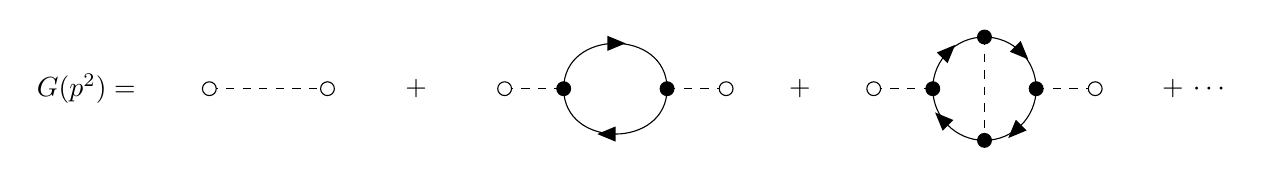
\begin{tikzpicture}[scale=1.25]
            \begin{feynman}
                \vertex (a);
                \vertex[right = of a] (b);
                \diagram*{
                    (a) -- [scalar] (b);
                };
                \draw[fill=white] (a) circle(0.7mm);
                \draw[fill=white] (b) circle(0.7mm);
            \end{feynman}
        \node at (2.1, 0) {+};
        \begin{scope}[xshift=3cm]
            \begin{feynman}
                \vertex (a) at (0,0);
                \vertex (b) at (0.6, 0);
                \vertex (c) at (1.65, 0);
                \vertex (d) at (2.25, 0);
                \diagram*{
                    (a) -- [scalar] (b) --[fermion, half left] (c) -- [scalar] (d);
                    (b) --[anti fermion, half right] (c);
                };
                \draw[fill=white] (a) circle(0.7mm);
                \draw[fill=white] (d) circle(0.7mm);
                \draw[fill=black] (c) circle(0.7mm);
                \draw[fill=black] (b) circle(0.7mm);
            \end{feynman}
        \end{scope}
        \node at (6, 0) {+};
        \begin{scope}[xshift=6.75cm]   
            \begin{feynman}
                \vertex (a) at (0,0);
                \vertex (b) at (0.6, 0);
                \vertex (c) at (1.65, 0);
                \vertex (d) at (2.25, 0);
                \vertex (up) at (1.125, 0.525);
                \vertex (dw) at (1.125, -0.525);
                \diagram*{
                    (a) -- [scalar] (b) --[fermion, quarter left] (up) --[fermion, quarter left] (c) --[scalar] (d);
                    (b) --[anti fermion, quarter right] (dw) -- [anti fermion, quarter right] (c);
                    (up) --[scalar] (dw);
                };
                \draw[fill=white] (a) circle(0.7mm);
                \draw[fill=white] (d) circle(0.7mm);
                \draw[fill=black] (c) circle(0.7mm);
                \draw[fill=black] (b) circle(0.7mm);
                \draw[fill=black] (up) circle(0.7mm);
                \draw[fill=black] (dw) circle(0.7mm);
            \end{feynman}
            \node at (3.25,0) {+ \(\cdots\) };
        \end{scope}
        \node at (-1.25,0) {\(G(p^2) = \)};
    \end{tikzpicture}
\end{figure} 

which is just as we had shown above, a free propagator plus some other terms. These other terms, in fact, have a simple structure as follows. We define the notion of a 1PI diagrams which stands for 1 Particle Irreducible diagrams. These are the diagrams which cannot be cut into two diagrams by cutting one line.

\begin{figure}[h]
    \centering
    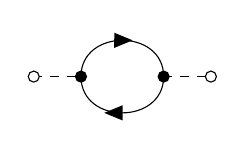
\begin{tikzpicture}[scale=1]
        \begin{scope}[xshift=0cm]
            \begin{feynman}
                \vertex (a) at (0,0);
                \vertex (b) at (0.6, 0);
                \vertex (c) at (1.65, 0);
                \vertex (d) at (2.25, 0);
                \diagram*{
                    (a) -- [scalar] (b) --[fermion, half left] (c) -- [scalar] (d);
                    (b) --[anti fermion, half right] (c);
                };
                \draw[fill=white] (a) circle(0.7mm);
                \draw[fill=white] (d) circle(0.7mm);
                \draw[fill=black] (c) circle(0.7mm);
                \draw[fill=black] (b) circle(0.7mm);
            \end{feynman}
        \end{scope}
    \end{tikzpicture}
\end{figure}

this is a 1PI diagram, but 

\begin{figure}[h]
    \centering
    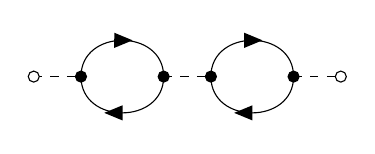
\begin{tikzpicture}[scale=1]
        \begin{scope}[xshift=0cm]
            \begin{feynman}
                \vertex (a) at (0,0);
                \vertex (b) at (0.6, 0);
                \vertex (c) at (1.65, 0);
                \vertex (d) at (2.25, 0);
                \vertex (e) at (3.3, 0);
                \vertex (f) at (3.9, 0);
                \diagram*{
                    (a) -- [scalar] (b) --[fermion, half left] (c) -- [scalar] (d) --[fermion, half left] (e) -- [scalar] (f) ;
                    (b) --[anti fermion, half right] (c);
                    (d) --[anti fermion, half right] (e);
                };
                \draw[fill=white] (a) circle(0.7mm);
                \draw[fill=white] (f) circle(0.7mm);
                \draw[fill=black] (c) circle(0.7mm);
                \draw[fill=black] (d) circle(0.7mm);
                \draw[fill=black] (e) circle(0.7mm);
                \draw[fill=black] (b) circle(0.7mm);
            \end{feynman}
        \end{scope}
    \end{tikzpicture}
\end{figure}

is not a 1PI diagram, since we can break the internal scalar propagator to get two diagrams. We define \(-i\Sigma(p^2)\) to be the sum of all 1PI diagrams 

\begin{figure}[H]
    \centering
    \begin{tikzpicture}
        \begin{feynman}
                \vertex (a) at (0,0);
                \vertex (b) at (1,0);
                \vertex (c) at (2.5,0);
                \vertex (d) at (3.5,0);
                \diagram*{
                    (b) --[scalar] (a);
                    (c) --[scalar] (d);
                };
                \draw[pattern={Lines[angle=-45,distance=4pt]}, pattern color=black!30] (1.75,0) circle(0.75cm) ;
                \draw[fill=white] (a) circle(1mm); 
                \draw[fill=white] (d) circle(1mm); 
            \end{feynman}
            \node at (4.75,0) {\(=-i\Sigma(p^2)\)};
            \node at (1.75,0) {1PI};
    \end{tikzpicture}
\end{figure}

The propagator therefore looks like 
\begin{figure}[H]
    \centering
    \begin{tikzpicture}[scale=1.15]
            \begin{feynman}
                \vertex (a);
                \vertex[right = of a] (b);
                \diagram*{
                    (a) -- [scalar] (b);
                };
                \draw[fill=white] (a) circle(0.7mm);
                \draw[fill=white] (b) circle(0.7mm);
            \end{feynman}
        \node at (1.65, 0) {+};
        \begin{scope}[xshift=2cm]
            \begin{feynman}
                \vertex (a) at (0,0);
                \vertex (b) at (0.5, 0);
                \vertex (c) at (1.5, 0);
                \vertex (d) at (2, 0);
                \diagram*{
                    (a) -- [scalar] (b);
                    (c) -- [scalar] (d);
                };
                \node at (1,0) {1PI};
                \draw[pattern={Lines[angle=-45,distance=4pt]}, pattern color=black!30] (1,0) circle(0.5cm) ;
                \draw[fill=white] (a) circle(0.7mm);
                \draw[fill=white] (d) circle(0.7mm);
            \end{feynman}
        \end{scope}
        \node at (4.35, 0) {+};
        \begin{scope}[xshift=4.75cm]   
            \begin{feynman}
                \vertex (a) at (0,0);
                \vertex (b) at (0.5, 0);
                \vertex (c) at (1.5, 0);
                \vertex (d) at (2, 0);
                \vertex (e) at (3, 0);
                \vertex (f) at (3.5, 0);
                \diagram*{
                    (a) -- [scalar] (b);
                    (c) --[scalar] (d);
                    (e) --[scalar] (f);
                };
                \node at (1,0) {1PI};
                \draw[pattern={Lines[angle=-45,distance=4pt]}, pattern color=black!30] (1,0) circle(0.5cm) ;
                \node at (2.5,0) {1PI};
                \draw[pattern={Lines[angle=-45,distance=4pt]}, pattern color=black!30] (2.5,0) circle(0.5cm) ;
                \draw[fill=white] (a) circle(0.7mm);
                \draw[fill=white] (f) circle(0.7mm);
            \end{feynman}
        \end{scope}
        \node at(8.6, 0) {+};
        \begin{scope}[xshift=9cm]   
            \begin{feynman}
                \vertex (a) at (0,0);
                \vertex (b) at (0.5, 0);
                \vertex (c) at (1.5, 0);
                \vertex (d) at (2, 0);
                \vertex (e) at (3, 0);
                \vertex (f) at (3.5, 0);
                \vertex (g) at (4.5, 0);
                \vertex (h) at (5, 0);
                \diagram*{
                    (a) -- [scalar] (b);
                    (c) --[scalar] (d);
                    (e) --[scalar] (f);
                    (g) --[scalar] (h);
                };
                \node at (1,0) {1PI};
                \draw[pattern={Lines[angle=-45,distance=4pt]}, pattern color=black!30] (1,0) circle(0.5cm) ;
                \node at (2.5,0) {1PI};
                \draw[pattern={Lines[angle=-45,distance=4pt]}, pattern color=black!30] (2.5,0) circle(0.5cm) ;
                \node at (4,0) {1PI};
                \draw[pattern={Lines[angle=-45,distance=4pt]}, pattern color=black!30] (4,0) circle(0.5cm) ;
                \draw[fill=white] (a) circle(0.7mm);
                \draw[fill=white] (h) circle(0.7mm);
            \end{feynman}
        \end{scope}
        \node at (14.75,0) {+ \(\cdots\) };
    \end{tikzpicture}
\end{figure}

and this can be summed to get 
\begin{equation*}
    \frac{-i}{p^2 - m^2 + i\epsilon} + \left( \frac{-i}{p^2 - m^2 + i\epsilon}(-i\Sigma(p^2))\frac{-i}{p^2 - m^2 + i\epsilon}\right) + \left(\frac{-i}{p^2 - m^2 + i\epsilon}\left((-i\Sigma(p^2))\frac{-i}{p^2 - m^2 + i\epsilon}\right)^2 \right) + \cdots
\end{equation*}
which forms a geometric series, whose sum looks like 
\begin{equation*}
    \displaystyle \frac{\displaystyle \frac{-i}{p^2 - m^2 + i\epsilon}}{\displaystyle 1 - \frac{\Sigma(p^2)}{p^2 - m^2 + i\epsilon}} = \frac{-i}{p^2 - m^2 + i\epsilon} \times \frac{p^2 - m^2 + i\epsilon}{p^2 - m^2 - \Sigma(p^2) + i\epsilon} = \frac{1}{p^2 - m^2 - \Sigma(p^2) + i\epsilon}
\end{equation*}
\(\Sigma(p^2)\) is called the self energy, and this is sensitive to the loop diagrams, and our renormalisation requirement is to set the counterterm such that the propagator has a pole at \(p^2 = m^2\) with residue \(1\). For \(\Sigma(p^2)\), the pole condition simply reads \(\Sigma(m^2) = 0\). We also need to see what the condition about the residue looks like for \(\Sigma\). To do that, we can expand \(\Sigma\) around \(p^2 = m^2\) to get  
\begin{equation*}
    \Sigma(p^2) = \Sigma(m^2) + (p^2 - m^2)\frac{d}{dp^2}\Sigma(m^2) + \text{hots (higher order terms)}
\end{equation*}
Substituting this, we get the propagator to be
\begin{equation*}
    \frac{1}{\displaystyle(p^2 - m^2) - (p^2 - m^2)\frac{d}{dp^2}\Sigma(m^2) + \text{hots} + i\epsilon} = \frac{1}{p^2 - m^2}\frac{1}{\displaystyle 1-\frac{d}{dp^2}\Sigma(m^2) + \text{hots}}
\end{equation*}
giving the residue at \(p^2 = m^2\) to be \(\left(\displaystyle 1-\frac{d}{dp^2}\Sigma(m^2)\right)^2\). Therefore, for the residue of the pole to be unchanged, we require 
\begin{equation*}
    \frac{d}{dp^2}\Sigma(p^2)\bigg|_{p^2 = m^2} = 0
\end{equation*}








\end{document}
